% !TXS template
\documentclass[german]{article}
\usepackage[T1]{fontenc}
\usepackage[utf8]{inputenc}
\usepackage{lmodern}
\usepackage[a4paper]{geometry}
\usepackage{babel}

\usepackage{amsmath}
\usepackage{amsfonts}
\usepackage{amssymb}
\usepackage{amsthm}

\usepackage{mathtools}

\usepackage{tipa}
\usepackage{stmaryrd}

\usepackage{aligned-overset}

\usepackage{accents}

\title{Mathematische Logik 2:\\Vorlesungmitschrift}
\author{Erich Grädel\\\small{(Mitschrift von Theodor Teslia)}}
\date{}


\newtheoremstyle{break}
{\topsep}{\topsep}%
{}{}%
{\bfseries}{}%
{\newline}{}%

\theoremstyle{break}
\newtheorem{example}{Beispiel}[section]

\newtheoremstyle{def_style}
{\topsep}{\topsep}%
{}{}%
{\bfseries}{}%
{\newline}{}%

\theoremstyle{def_style}
\newtheorem{definition}{Definition}[section]

\theoremstyle{def_style}
\newtheorem{satz}{Satz}[section]

\newtheoremstyle{lemma_style}
{\topsep}{\topsep}%
{}{}%
{\itshape}{:}%
{ }{}%

\theoremstyle{lemma_style}
\newtheorem{lemma}{Lemma}[subsection]

\usepackage{tikz}
\usetikzlibrary{arrows.meta}

\newcommand{\Pot}[1]{\mathcal{P}(#1)}

\renewcommand{\phi}{\varphi}

\newcommand{\A}{\mathfrak{A}}
\newcommand{\B}{\mathfrak{B}}
\newcommand{\C}{\mathfrak{C}}
\newcommand{\D}{\mathfrak{D}}

\newcommand{\N}{\mathbb{N}}
\newcommand{\R}{\mathbb{R}}
\newcommand{\Q}{\mathbb{Q}}

\renewcommand{\preceq}{\preccurlyeq}
\renewcommand{\succeq}{\succcurlyeq}

\def\opencorner{\text{\textopencorner}}
\def\closecorner{\text{\textcorner}}

\begin{document}

\maketitle

\tableofcontents

\clearpage

\section{Mengenlehre}

\glqq Aus dem Paradies, das Cantor uns geschaffen, soll uns niemand vertreiben können.\grqq{}\\
(David Hilbert, 1926) 

\subsection{Mengen und Klassen}

Reine Mengen sind Kollektion an Objekten, die ebenfalls wieder Mengen sind, als Alternative lassen sich Mengen ausgehend von Urelementen definieren.
\\
Wie führt die Mathematik Objekte ein?
\begin{itemize}
	\item Explizite Konstruktion aus schon vorhandenen Objekten, bspw. Konstruktion der rationalen, reellen und komplexen Zahlen, ausgehend von den ganzen und natürlichen.
	\item Axiomatisches formulieren von gewünschten Eigenschaften der Objekte und betrachte alle Objekte, die die Eigenschaften erfüllen, bspw. Gruppen, Vektorräume, ...
\end{itemize}

\begin{definition}[Mengen]
	Intuitiv sind Mengen \textit{Kollektionen von Objekten}, die selbst wieder Mengen sind. 
	
	$a\in b$: $a$ ist ein Element in der Menge $b$.
	
	$a \subseteq b$: Jedes Element von $a$ ist auch in $b$.
	\\
	Eine Konstruktive Definition von aller Menge könnte wie folgt aussehen:\\ $\{\emptyset\}, \{\emptyset,\{\emptyset\}\}, \{\{\emptyset\}\}$ \textit{usw.}
	Problem: Wie sieht dieses \textit{usw.} aus?
\end{definition}


Mengen lassen sich auch als Bäume darstellen. Dies lässt sich in Abbildung \ref{Mengenbaum} Beispielhaft für die Menge $\{\; \emptyset, \; \{\emptyset\}, \; \{\emptyset,\{\emptyset\}\}\;\}$ erkennen. 

\begin{figure}[h]
	\begin{center}
		\begin{tikzpicture}
			\node {$\bigcirc$}
			child {node {$\emptyset$}}
			child {node {$\bigcirc$}
				child {node {$\emptyset$}}}
			child {node {$\bigcirc$}
				child {node {$\emptyset$}}
				child {node {$\bigcirc$}
					child {node {$\emptyset$}}}};
		\end{tikzpicture}
	\end{center}
\caption{Darstellung der Menge $\{\; \emptyset, \; \{\emptyset\}, \; \{\emptyset,\{\emptyset\}\}\;\}$ als Baum}
\label{Mengenbaum}
\end{figure}

\begin{definition}[Hereditär endliche Mengen]
	Die \textit{hereditär endlichen Mengen} ($HF$) bilden eine Miniaturversion der Mengenlehre. Es gilt $HF_0\subset HF_1 \subset HF_2 \subset \dots$. Definiert sind diese Mengen induktiv als $HF_0\coloneqq \emptyset$ und $HF{n+1}\coloneqq \{x : x\subseteq HF_n\}$, so dass $HF_{n+1}$ die Potenzmenge von $HF_n$ ist.
	
	Eine Menge ist hereditär endlich, wenn sie Element einer Menge $HF_n$ für ein $n$ ist. Weiter wird $HF\coloneqq\{x : x \in HF_n \text{ für ein }n\in \mathbb{N}\}$ definiert.
	Dies wirft folgende Frage auf: Ist $HF$ eine Menge? 
\end{definition}

Die ersten $HF$ Mengen lauten $HF_0=\emptyset$, $HF_1=\{\emptyset\}$, $HF_2=\{\emptyset,\{\emptyset\}\}$, \\ $HF_3=\{\emptyset, \{\emptyset\}, \{\{\emptyset\}\}, \{\emptyset,\{\emptyset\}\}\}$. Es lässt sich erkennen, dass $HF_n\subset HF_{n+1}$ und $HF_n\in HF_{n+1}$ für ein beliebiges $n$. Auch ist es möglich zu folgern, dass $HF_n$ endlich viele Elemente besitzt und jede Menge $a\in HF_{n+1}$ die Gestalt $a=\{b_0,\dots,b_{k-1}\}$ mit $b_0,\dots,b_{k-1}\in HF_n$. Außerdem gilt, dass $HF$ nicht hereditär endlich ist.

\begin{definition}[Natürliche Zahlen]
	Eine \textit{natürliche Zahl} $n$ ist definiert als $[n]\coloneqq\{[0],\dots,[n-1]\}$, wobei $[0]=\emptyset$ gilt. Die Menge der natürlichen Zahlen $\mathbb{N}$ lässt sich nun als $\mathbb{N}\coloneqq\{[n] : n \text{ eine nat. Zahl}\} \notin HF$. Eine Folgerung ist $[n]\in HF_{n+1}\setminus HF_n$.
\end{definition}

\subsubsection{Axiomensysteme für die Mengenlehre}

Das Modell der Mengenlehre besteht aus einer Kollektion $\mathcal{S}$ von Objekten, die wir Mengen nennen und einer Beziehung $\in$ zwischen diesen Objekten, so dass alle Axiome des Axiomensystems erfüllt werden.

\begin{definition}[Extensionalitätsaxiom (Ext.)]
	Zwei Mengen sind gleich, genau dann, wenn sie die selben Elemente haben. In einer Formel aus der Prädikatenlogik mit Signatur $\{\in\}$ wäre dies $\forall x \forall y (x=y \leftrightarrow \forall z (z \in x \leftrightarrow z \in y))$.
	\label{ExtAxiom}
\end{definition}

Die \textit{Konsistenz} des Axiomensystems der Mengenlehre beschreibt, ob es ein Modell des Axiomensystems gibt oder ob dieses Widersprüchlich ist. Es ist nicht möglich, die Konsistenz unseres Axiomensystems zu beweisen.

Das Axiomensystem der Mengenlehre ist \textit{Vollständig}, wenn alle Modelle \glqq gleich \grqq{} sind, in dem Sinn, dass die gleichen Eigenschaften gelten. Es gibt kein vollständiges Axiomensystem für die Mengenlehre.
\\
\\
Nehmen wir an, dass $(\mathcal{S},\in)$ ein beliebiges, aber festes Modell der Mengenlehre ist. Die Axiome sollen regeln, welche Kollektionen von Elementen aus $\mathcal{S}$ selbst wieder Elemente von $\mathcal{S}$, also Mengen sind. Dabei werden Kollektionen \textit{Klassen} genannt und Klassen, die keine Mengen sind, werden als \textit{echte Klassen} bezeichnet.

\begin{definition}[Die naive Mengenlehre]
	Das Axiomensystem der naiven Mengenlehre besitzt zwei Axiome. Zum einen das Extensionalitätsaxiom (siehe Definition \ref{ExtAxiom}) und das Axiomenschema der vollen Komprehension. Dieses besagt, dass sich für jede Formel $\psi(x)$ die Menge $\{x : \psi(x)\}$ bilden lässt: $\exists z \forall z(x \in z \leftrightarrow \psi(x))$.
\end{definition}

\begin{satz}[Zermelo-Russel Paradoxon]
	Die naive Mengenlehre ist inkonsistent.
	
	Sei $\psi(x)\coloneqq x\notin x$. Nach dem Komprehensionsschema muss nun folgende Formel gelten: $\exists z \forall x(x\in z \leftrightarrow x\notin x)$, aus welcher die Menge $z=\{x : x\notin x\}$ folgt. Eine solche Menge kann aber nicht existieren, da sonst $z\in z \Leftrightarrow z \notin z$ gelten müsste. Es folgt, dass $\{x:x\notin x\}$ immer einer echte Klasse sein muss.
\end{satz}

\begin{definition}[Das Axiomensystem ZFC]
	Das Axiomensystem ZFC (\textbf{Z}ermelo-\textbf{F}raenkel-\textbf{C}hoice) ist das heutzutage benutzte Axiomensystem. Es besitzt die folgenden Axiome:
	\begin{itemize}
		\item Das Extensionalitätsaxiom
		\item Das Aussonderungsaxiom: $\forall z \exists y \forall x (x\in y \leftrightarrow(x\in z \land \psi(x)))$. Dieses ist eine schwächere Version des Komprehensionsschemas, bei dem eine Menge aus bereits bestehenden Menge ausgewählt wird.
		\item Das Erzeugungsaxiom (Kreationsaxiom): Für jede Menge $x$ ex. eine \textit{Stufe} $s\in S$ mit $x\in s$.
		\item Das Unendlichkeitsaxiom: Es gibt eine \textit{Limesstufe} und damit eine unendliche Menge.
		\item Das Ersetzungsaxiom: Für jede Funktion $F:\mathcal{S}\to \mathcal{S}$ mit der Eigenschaft, dass wenn $Def(F)$ eine Menge ist, ist auch $Bild(F)$ eine Menge.
		\item Das Auswahlaxiom: Auf jeder Menge ex. eine \textit{Auswahlfunktion}
	\end{itemize}
\end{definition}

\begin{definition}[Klassenoperatoren]
	Seien $A, B$ Klassen.
	
	$A \subseteq B$: Jede Menge aus $A$ ist auch in $B$.
	
	$\bigcap A\coloneqq\{x : x\in y \text{ für alle } y \in A\}$
	
	$A \cap B \coloneqq \{x : x\in A \text{ und } x \in B\}$
	
	$A \setminus B \coloneqq \{x : x \in A \text{ aber } x \notin B\}$
\end{definition}

Für eine Formel $\psi(x)$ kann $\{x : \psi(x)\}$ entweder eine Menge oder eine echte Klasse sein. Somit lässt sich das Aussonderungsaxiom umformulieren: Für jede Menge $a$ und jede Klasse $A$ ist $a \cap A$ eine Menge. Daraus folgt, dass auch $a \setminus A$ eine Menge sein muss, dass $\bigcap A$ eine Menge ist, falls $A$ mindestens eine Menge enthält und, dass $\bigcap \emptyset = S$ keine Menge ist.

\subsection{Stufen und Geschichten}

Eine mögliche Methode zur Definition der gesamten Klasse aller Mengen ist es, die induktive Konstruktion der $HF$ zu erweitern. So ist $\mathcal{S}$ dann die Vereinigung einer aufsteigenden Folge von Mengen $S_\alpha$, welche wir die Stufen von $\mathcal{S}$ nennen. Es gilt $S_0\coloneqq \emptyset$ und für die bereits definierte Stufe $S_\alpha$ setzen wir $S_{\alpha +1}\coloneqq\{x : x\in S_\alpha\}$.

Sobald eine unendliche Folge von solchen Stufen definiert wurde, lässt sich eine neue Stufe als Vereinigung aller bisherigen Stufen definieren.\\

$S_0=HF_0=\emptyset$, $S_1=HF_1$, $\dots$, $S_n=HF_n$

$S_\omega \coloneqq \bigcup\limits_n S_n = \bigcup\limits_n HF_n = HF$

$S_{\omega+1}\coloneqq\{x : s\in S_\omega\}$, $\dots$

$S_{\omega+\omega}\coloneqq\{x : x \in S_{\omega+n} \text{ für ein } n\}$ \textit{usw.}

\begin{definition}[Die Akkumulation]
	Sei $A$ eine Klasse. Die \textit{Akkumulation} von $A$ ist $acc(A)\coloneqq\{x : (\exists y \in A) x\in y\lor x \subset y\})$.
\end{definition}

Da für eine Klasse $A$ und ein Element $a\in A$ natürlich gilt, dass $a \subset a$, gilt auch $a\in acc(A)$ und somit $A\subseteq acc(A)$.

\begin{definition}[Geschichten]
	Eine \textit{Geschichte} ist eine Klasse $H$, so dass für alle $a\in H$ gilt $acc(a\cap H)=a$.
\end{definition}

Die Stufe mit Geschichte $H$ ist $S\coloneqq acc(H)$.

\begin{example}[Beispiele zu Geschichten und Stufen]
	Im Folgenden soll für einige Mengen ihre Akkumulation gezeigt werden und bewiesen, dass es sich bei diesen auch um Geschichten handelt.
	\begin{itemize}
		\item $acc(\emptyset)=\emptyset$. $\emptyset$ ist eine Geschichte und die Stufe mit Geschichte $\emptyset$ ist $\emptyset$.
		\item $\{\emptyset\} = [1] = HF_1 = \{HF_0\}$: $acc(\{\emptyset\}) = \{\emptyset\}$. 
		$\{\emptyset\}$ ist auch eine Geschichte, denn für das einzige Element $\emptyset$ gilt $acc(\emptyset \cap \{\emptyset\})=acc(\emptyset)=\emptyset$. 
		Die Stufe mit Geschichte $\{\emptyset\}$ ist $\{\emptyset\}$.
		\item $\{\emptyset, \{\emptyset\}\}=[2]=HF_2=\{HF_0, HF_1\}$: $acc(HF_2)=HF_2$.
		$HF_2$ ist eine Geschichte, denn $acc(\emptyset \cap \{\emptyset, \{\emptyset\}\})=acc(\emptyset)=\emptyset$ und $acc(\{\emptyset\}\cap \{\emptyset, \{\emptyset\}\})=acc(\{\emptyset\})=\{\emptyset\}$. Die Stufe mit Geschichte $\{\emptyset, \{\emptyset\}\}$ ist $\{\emptyset, \{\emptyset\}\}$.
	\end{itemize}
\label{GeschichtenBsp}
\end{example}

Dies wirft die Frage auf, ob es eine Verallgemeinerung gibt. Demnach soll nun überprüft werden, ob $[n]$ eine Geschichte ist, für jedes $n$ in den natürlichen Zahlen. Für $k<n$ müsste gelten, dass $acc([n]\cap[k])=acc([k])\stackrel{!}{=}[k]$. 
Aber $acc([k])$ enthält alle Teilmengen von $[k-1]$, für $k=4$ also alle Teilmengen von $\{[0],[1],[2]\}$, demnach auch $\{[0], [2]\}$. Es gilt aber, dass $\{[0],[2]\}\notin [k]$ und es folgt $acc([k])\neq[k]$. Für $n \geq 3$ ist $n$ also keine Geschichte.

Ist $HF_n$ eine Geschichte? Nein, denn $[n-1]\in HF_n$ und $acc([n-1]\cap HF_n)=acc([n-1])\neq[n-1]$.

Aber $G_n\coloneqq\{HF_0,\dots,HF_{n-1}\}$ ist eine Geschichte mit Stufe $HF_n$. Für $n=0,1,2$ wurde dies schon in Beispiel \ref{GeschichtenBsp} gezeigt. Sei dies für $G_n$ bereits bewiesen, wir zeigen dies nun für $G_{n+1}=G_n\cup\{HF_n\}$.
$G_{n+1}$ ist eine Geschichte, wenn für alle $k \leq n$ gilt: $acc(HF_k\cap G_{n+1})=HF_k$.
$HF_k \cap G_{n+1} = \{HF_0,\dots,HF_{k-1}\}=G_k$ und per Induktionsvoraussetzung gilt $acc(G_k)=HF_k$.

Also ist $G_{n+1}$ eine Geschichte. Die Stufe mit Geschichte $G_{n+1}$ ist $acc(G_{n+1})=acc(G_n\cup \{HF_n\})=acc(GF_n)\cup HF_n \cup \{x : x\subseteq HF_n\}=HF_n\cup HF_n \cup HF_{n+1} = HF_{n+1}$.

Dies gibt die Idee für die Rückrichtung: Für jede Stufe $S_\alpha$ soll gelten, dass sie die Geschichte $H(S_\alpha)=\{S_\beta : \beta < \alpha\}$ hat.

\begin{definition}[Minimales Element]
	Eine Menge $m\in A$ ist ein \textit{minimales Element} von $A$, wenn $m\cap A=\emptyset$, d.h. es gibt kein $a\in A$ mit $a\in m \in A$.
	
	Eine Menge $a$ ist fundiert, wenn jede Menge $b$ mit $a\in b$ ein minimales Element enthält. Der fundierte Teil von $A$ ist $fd(A)\coloneqq\{x\in A : x \text{ ist fundiert}\}$.
\end{definition}

\begin{example}[Beispiele für minimale Elemente und Fundiertheit]
	$\emptyset$ ist fundiert.
	
	$\{\emptyset\}$ ist ebenfalls fundiert. Sei $\{\emptyset\}\in b$. Wenn $\{\emptyset\}\cap b =\emptyset$ ist $\{\emptyset\}$ das minimale Element. Andernfalls ist $\{\emptyset\}\cap b=\{\emptyset\}$ und $\emptyset$ ist das minimale Element von $b$.
\end{example}

\begin{satz}
	Wenn $H$ eine Geschichte ist, dann enthält jede nicht-leere Teilmenge von $H$ ein minimales Element.
\end{satz}
\begin{proof}
	Es sei $a\in b \subset H$ und $c=\{fd(x) : x \in a\cap b\}=\{y:y=fd(x)\text{ für } x\in a \cap b\}$.
	Wenn $c=\emptyset$, dann ist $a\cap b = \emptyset$ und $a$ ist das minimale Element von $b$.
	Sei $c\neq \emptyset$. Wir wollen zeigen, dass $c\subseteq fd(a)$.
	
	\begin{lemma}
		Sei $H$ eine Geschichte, mit $a,b\in H$ und $a\in b$. Dann muss $fd(a)\in fd(b)$ gelten. Ansonsten wäre $fd(a)\in acc(b\cap H)=b$, da $fd(a)\subseteq a \in b \cap H$. Also gilt mit der Voraussetzung $fd(a)\in b \setminus fd(b)$. Demnach ex. eine Menge $x$ mit $fd(a)\in x$ ohne minimale Elemente. Speziell ist $fd(a)$ kein minimales Element von $x$, d. h. $fd(a)\cap x \neq \emptyset$. Sei $y\in fd(a)\cap x$. Da $y\in fd(a)$ ist $y$ fundiert. Da $y \in x$ hat $x$ ein minimales Element. Dies ist ein Widerspruch zu der Aussage, dass $fd(a)\in b \setminus fd(b)$, es muss also $fd(a)\in fd(b)$ gelten.
	\end{lemma}

	Sei $y\in c$. Dann ist $y = fd(x)$ für ein $x\in a\cap b$. Aus dem Lemma folgt, dass $y\in fd(a)$. Also $c\subseteq fd(a)$.
	
	Wenn $y\in c \subseteq fd(a)$, dann ist $y$ fundiert und $c$ hat ein minimales Element $z$. Nach der Definition von $c$ ist dann $z=fd(x)$ für ein $x\in a\cap b$.
	
	Behauptung: $x$ ist das minimale Element von $b$. Wenn nicht, dann existiert ein $u \in x \cap b$. Da $u \in x \in a\cap b\subseteq a\cap H$ und $a\in H$ ist auch $u$ in $acc(a\cap H)=a$. Also $u \in a\cap b$ und daher $fd(u)\in c = \{fd(x):x\in a\cap b\}$. Aus dem Lemma folgt $fd(u)\in fd(x)$, da $u\in b \subseteq H$ und $x\in b \subseteq H$. Also $fd(u)\in fd(x)\cap c \neq \emptyset$. Also ist $z=fd(x)$ nicht minimales Element von $c$. Dies ist ein Widerspruch.
\end{proof}

\begin{satz}
	Sei $H$ eine Geschichte. Jedes Element $a\in H$ ist eine Stufe mit Geschichte $H\cap a$.
	\label{ElementVonGeschichteIstStufe}
\end{satz}
\begin{proof}[a)]
	Da $H$ eine Geschichte ist, gilt $a=acc(H\cap a)$. Wenn $H\cap a$ eine Geschichte ist, dann ist $a$ die zugehörige Stufe. Sei $b\in H \cap a$. Dann $b\subseteq a$, da $c\in b \in H\cap a \Rightarrow c \in acc(H\cap a)=a$ und also $H\cap b = (H\cap a)\cap b$. Da $b\in H$ gilt, dass $b=acc(H\cap b) = acc((H\cap a)\cap b)$. Also ist $H\cap a$ eine Geschichte.
\end{proof}

\begin{definition} [Transitive und Erbliche Klassen]
	Eine Klasse ist
	\begin{itemize}
		\item \textit{transitiv}, wenn für alle $a\in b\in A$ auch $a\in A$ gilt, also jedes Element von $A$ ist auch Teilmenge von $A$.
		\item \textit{erblich}, wenn für alle $a\subset b \in A$ auch $a\in A$ gilt.
	\end{itemize}
\end{definition}

\begin{satz}
	Sei $S$ eine Stufe mit Geschichte $H$.
	\begin{itemize}
		\item[a)] $S$ ist erblich und transitiv.
		\item[b)] $S=\{x : x\subseteq s \text{ für eine Stufe } s\in S\}$
		\item[c)] $H(S)\coloneqq\{s\in S : s\text{ ist Stufe}\}$ ist eine Geschichte von $S$.
	\end{itemize}
\end{satz}
\begin{proof}
	a) Sei $b\in S=acc(H)$, es ist zu zeigen, dass $a\in b\Rightarrow a\in S$ und $a\subseteq b \Rightarrow a\in S$. Sei $c=\{s\in H : b\in s \lor b \subseteq s\}\subseteq H$ Da $b\in acc(H)$ ist $c\neq \emptyset$ und daher existiert ein $s\in c$ mit $s\cap c=\emptyset$. Nach Definition von $c$ gilt $b\in s$ oder $b\subseteq s$. 
	
	Behauptung: $b\notin s$, da sonst $b\in s = acc(H\cap s)$, also ex. $z\in H\cap s$ mit $b\subseteq z$ oder $b\in z$. Dann ist aber $z\in c\cap s\neq \emptyset$, also ein Widerspruch. Es muss also $b\subseteq s$ gelten. 
	\begin{itemize}
		\item $a\in b \Rightarrow a \in b \subset s=acc(H\cap s)\subset(H)=S\Rightarrow a\in S$
		\item $a\subseteq b\Rightarrow a\subseteq b \subseteq s\in H \Rightarrow a\in acc(H)=S$
	\end{itemize}

	b) \glqq$\supseteq$\grqq: $a\subseteq s \in S\stackrel{a)}{\Rightarrow}a\in S$
	
	\glqq$\subseteq$\grqq{}: Sei $a\in S=acc(H)$. Es gilt $s\in H$ mit $a\in s$ oder $a\subseteq s$. Nach dem Satz \ref{ElementVonGeschichteIstStufe} ist $s$ eine Stufe mit Geschichte $H\cap s$ und daher erblich und transitiv (nach a)). Wenn $a\in s$, dann $a\subseteq s$. Also $a\subseteq s\in H\subseteq S$ und daher $a\in\{x : x\subseteq s \text{ für ein } s\in S\}$.
	
	c) $acc(H(S))=\{x : (\exists s\in H(S)) x\in s \lor x\in s\} = \{x : (\exists s \in S) s \text{ ist Stufe}, x\subseteq s\in\}\stackrel{b)}{=}S$. $H(S)$ ist eine Geschichte. $H(S)\cap s=\{s\in S\cap s : x \text{ Stufe}\}=\{x\in s : x \text{ Stufe}\}$. Dann $acc(H(S)\cap s)=\{y : (\exists s'\in s) s' \text{ ist Stufe}, y\subseteq s'\}\stackrel{b)}{=}S$
 \end{proof}

Aus diesen Sätzen folgt, dass für die Geschichte $H$ einer Stufe $S$ gilt, dass $H \subset H(S)$. Sei $a\in H$. Es folgt $a\in S=acc(H)$ und $a$ ist eine Stufe mit Geschichte $H\cap a$, also $a\in H(S)$,

\begin{satz}
	Jede nicht-leere Klasse $A$ von Stufen hat ein minimales Element $s_0(A)$.
\end{satz}
\begin{proof}
	Sei $A\subset\{s : s \text{ ist eine Stufe}\}$, so dass kein $s\in s_0(A)\cap A$ existiert. Sei $s\in A$ und $x:=s\cap A$. Wenn $x=\emptyset$, dass $s_0(A)=s$. 
	Andernfalls ist $x\subseteq\{t \in s : t \text{ ist eine Stufe}\}$ eine nicht-leere Teilmenge einer Geschichte und hat daher ein minimales Element $m\in x$, so dass gilt $m\cap x = \emptyset$. 
	Setze $s_0(A)=m$, es folgt $s_0(A)\cap A=\emptyset$. Wäre nämlich $t \in s_0(A)\cap A=m\cap A$, da $t\in m \in x \subset s$, also $t \in s$, da $m$ transitiv ist, also $t\in x$. Es würde also ein $t\in m\cap x$ existieren. Widerspruch!
\end{proof}

\begin{satz}
	Seien $S, T$ Stufen, welche auch Mengen sind. Dann gilt entweder $S\in T$, $S=T$ oder $T \in S$.
\end{satz}
\begin{proof}
	Wenn nicht, dann ist die Klasse $A\coloneqq\{s : s \text{ ist Stufe und es gibt eine Stufe } t \text{ mit } s \notin t, s\neq t \text{ und } t \notin s\}$ nicht leer und enthält ein minimales Element $s_0=s_0(A)$. 
	Die Klasse $B\coloneqq\{t : t \text{ is eine Stufe, so dass } s_0 \notin t, s_0\neq t \text{ und } t \notin s_0\}$ muss dann ebenfalls ein minimales Element $t_0$ enthalten.
	Es gilt \boxed{s_0\notin t_0, s_0\neq t_0 \text{ und } t_0 \notin s_0}.
	Sei $s\in s_0$. Dann ist $s\neq t_0$, da sonst $t_0\in s_0$.
	Zweitens ist $t_0 \notin s$, da sonst $t_0\in s \notin s_0$ und damit $t_0\in s_0$.
	Wenn auch noch $s\notin t_0$ gelten würde, dann wäre $s\in A$ im Widerspruch zur Minimalität von $s_0$. Also muss $s\in t_0$. Aber damit ist gezeigt, dass $s_0\subseteq t_0$. Analog lässt sich zeigen, dass $t_0\subseteq s_0$ sein muss. Also $s_0=t_0$. Widerspruch!
\end{proof}

Aus dieser wichtigen Eigenschaft lassen sich einige Folgerungen feststellen. Seien $S, T$ Stufen aus $\mathcal{S}$.
\begin{enumerate}
	\item[a)] $S\notin S$
	\item[b)] $S\subseteq T \Leftrightarrow S=T \text{ oder } S \in T$
	\item[c)] $S\subseteq \text{ oder } T\subset S$
	\item[d)] $S\subsetneqq T \Leftrightarrow S\in T$
\end{enumerate}
\begin{proof}
	a) Wäre $S\in S$, wäre $A=\{s : s \text{ ist Stufe}, s\in s\}$ eine nicht-leere Klasse an Stufen, mit minimalem Element $s_0$, das heißt $s_0\cap A=\emptyset$. 
	Aber $s_0\in A$, wonach $s_0\in s_0$, was zur Folge hat, dass $s_0\in s_0\cap A\neq \emptyset$. Widerspruch!
	
	b) \glqq$\Leftarrow$\grqq: Wenn $S=T$, dann ist offensichtlich $S\subseteq T$ und wenn $S\in T$, dann gilt wegen der Transitivität auch $S\subseteq T$.
	
	\glqq $\Rightarrow$ \grqq: Wenn $S\neq T$ und $S\notin T$, dann muss $T\in S$ gelten, wenn nun aber $S\subseteq T$, dann ist $T\in S\subseteq T$, was ein Widerspruch zu Teil a) ist.
	
	c) Wenn $S\not\subseteq T$, dann muss wegen b) $S\notin T$ und $S\neq T$ gelten. Also ist $T\in S$ und daher auch $T\subseteq S$.
	
	d) $S\subsetneqq T \Leftrightarrow S\subseteq T \land S\neq T \Rightarrow S\in T$
\end{proof}

Statt $S\in T$, bzw. $S\subsetneqq T$ schreibt man oft $S<T$. Die so erzeugte lineare Ordnung von Stufen bezeichnet man als \textit{kumulative Hierarchie} und ist die durch $\in$ linear geordnete Kollektion aller Stufen.

Das \textit{Kreationsaxiom} besagt, dass zu jeder Menge $a$ eine Menge $s$ existiert, welche eine Stufe ist, mit $a\in s$. Aus diesem folgt, dass es zu jeder Stufe $s$ eine höhere Stufe $t$ mit $s\in t$ gibt, welche ebenfalls eine Stufe ist. Es lässt sich dadurch auch erkennen, dass $\mathcal{S}$ die Vereinigung aller Stufen ist. Wenn wir zudem akzeptieren, dass $\emptyset$ eine Menge ist, also $\mathcal{S}\neq \emptyset$, dann folgt, dass $HF\subset \mathcal{S}$ und, dass $\mathcal{S}$ selbst wieder eine Stufe mit der Geschichte $H(\mathcal{S})=\{s: s\text{ ist eine Stufe}\}$ ist.

\begin{definition}[Nachfolgerstufe]
	Eine Stufe $T$ ist die \textit{Nachfolgerstufe} zur Stufe $S$, wenn $S\in T$ und keine Stufe $T'$ existiert, mit $S\in T'\in T$.
\end{definition}

\begin{definition}[Limesstufe]
	Eine Stufe $S\neq \emptyset$ ist eine \textit{Limesstufe}, wenn sie keine Nachfolgerstufe ist.
\end{definition}

\begin{definition}
	Für jede Klasse $A$ ist $S(A)$ die kleinste Stufe mit $A\subseteq S$. Dies ist wohldefiniert, da jede nicht-leere Klasse von Stufen ein minimales Element besitzt. Es gilt $S(s)=s$ für jede Stufe $s$.
\end{definition}

Es gilt, dass $HF_{n+1}$ die Nachfolgerstufe von $HF_n$ ist.

Aus dem \textit{Aussonderungsaxiom} lassen sich weitere praktische Eigenschaften folgern. Sei $a$ eine Menge. Es lassen sich nun Elemente aussondern, so dass man die Mengen $\{a\}$, $acc(a)$ und $\bigcup a\coloneqq\{b : b\in x\text{ für ein } x \in a\}$ bilden kann.

Für eine Stufe $s$ mit $a\in s \in \mathcal{S}$ gilt:
\begin{itemize}
	\item $\{a\}=\{x\in s : x=a\}$
	\item $\{acc(a)\}=\{x\in s: (\exists b\in a)x\in b \lor x\subseteq b\}$
	\item $\bigcup a=\{b\in s : (\exists x\in a)b\in x\}$
\end{itemize}

Sei nun $A$ eine Klasse. Dann ist $S(A)$ die kleinste Stufe, so dass $A\subseteq S(A)$. Es lässt sich daraus auch leicht erkennen, dass für jede Stufe $s$ gilt $S(s)=s$.

\begin{lemma}
	Wenn $a\in b$, dann $S(a)\in S(b)$.
\end{lemma}
\begin{proof}
	Da $a\in b \subseteq S(b)=acc(H(S(b)))$ ex. $s\in S(b)$ mit $a\in s$ (und durch die Transitivität $a\subseteq s$), also ist $S(a)\subseteq s$ und daher $S(a)\subseteq s \in S(b)$ und da $S(b)$ erblich ist, folgt $S(a)\in S(b)$.
\end{proof}

\begin{lemma}
	$\mathcal{S}$ ist die einzige Stufe, welche ein echte Klasse ist.
	\label{EinzigeStufeDieKlasseIst}
\end{lemma}
\begin{proof}
	Sei $S$ eine Stufe, $S\neq \mathcal{S}$. Also ex. $a\in \mathcal{S}\setminus S$. Es folgt, dass $S(a)\notin S$, da sonst $a\subseteq S(a)\in S$ und daher $a\in S$. 
	Für Stufen $T \supseteq S(a)$ gilt daher $T \notin H(S)=\{s\in S : s \text{ ist Stufe}\}$. Also $H(S)\subseteq\{T : T \text{ ist Stufe}, T \in S(a)\}$. Da $S(a)$ und $H(S(a))$ mengen sind, ist auch $H(S)$ eine Menge und damit auch $S=acc(H(S))$.
\end{proof}

Daraus lässt sich folgern, dass die folgenden Aussagen für eine Klasse $A$ äquivalent sind:
\begin{enumerate}
	\item $A$ ist eine echte Klasse.
	\item $S(A)$ ist eine echte Klasse.
	\item $S(A)=\mathcal{S}$.
\end{enumerate}
\begin{proof}
	\textit{3. $\Rightarrow$ 1.}: Wenn $A$ eine Menge ist, ist auch $S(A)$ eine Menge. Nach Kontraposition gilt die Folgerung.
	
	\textit{1. $\Rightarrow$ 2.}: Wenn $S(A)$ eine Menge ist, ist auch $A=A\cap S(A)$ eine Menge. Nach Kontraposition gilt die Folgerung.
	
	\textit{2. $\Rightarrow$ 3.}: Dies wurde in Lemma \ref{EinzigeStufeDieKlasseIst} bewiesen.
\end{proof}

\begin{satz}
	Für jede Menge $a$ gilt $a\notin a$.
\end{satz}
\begin{proof}
	Es gelte $a\in a$. Dann $a\in a \subseteq S(a)§$. $S(a)=\{x : x\subseteq s \text{ für eine Stufe } s\in S(a)\}$, also existiert $s\in S(a)$ mit $a\subseteq s$. $S(a)$ ist aber die minimale Stufe, die $a$ als Teilmenge enthält. Widerspruch!
\end{proof}

Durch diesen Satz ist die Fundiertheit der Mengenlehre bewiesen.

\begin{satz}
	Jede nicht-leere Klasse enthält ein minimales Element.
\end{satz}
\begin{proof}
	Sei $A$ eine nicht-leere Klasse. $B=\{S(b) : b \in A\}$ ist die nicht-leere Klasse der Stufen in $A$ und hat ein minimales Element $s_0=S(b_0)$. D.h. $S(b_0)\cap B = \emptyset$. 
	Behauptung: $b_0$ ist das minimale Element von $A$. Andernfalls ex. $b_1\in b_0\cap A$. Da $b_1 \in b_0$ ist auch $S(b_1)\in S(b_0)$. Da $b_1\in A$ folgt $S(b_1)\in b$. Also $S(b_1)\in S(b_0)\cap B \neq \emptyset$. Widerspruch!
\end{proof}

\begin{lemma}
	Set $S\in \mathcal{S}$ eine Stufe. Die Nachfolgerstufe von $S$ ist $\Pot{S}$, wobei $\mathcal{P}$ die Potenzfunktion ist.
\end{lemma}
\begin{proof}
	Es gibt eine minimale Stufe $T$ mit $S\in T$. Nun ist zu zeigen, dass $\Pot{S}=T$.
	
	Aus $a\subseteq S\in T$ folgt wegen der Erblichkeit von $T$ auch $a\in T$. Also $\Pot{S}\subseteq T$. Sei $s \in T$ eine Stufe. $S\notin s$, da $T$ die Nachfolgerstufe von $S$ ist. Also gilt $S=s$ oder $s\in S$ und $s\subseteq S$. Für alle Stufen $s$ gilt $s\in T \Leftrightarrow s\subseteq S$. Nun gilt $T=\{x : x\subseteq s \text{ für eine Stufe } s\in T\}=\{x : x \subseteq s \text{ für eine Stufe } s\subseteq S\}=\{x : x \subseteq S\}=\Pot{S}$
\end{proof}

\begin{satz}
	Sei $S\neq \emptyset$ eine Stufe. Nun sind äquivalent:
	\begin{enumerate}
		\item $S$ ist eine Limesstufe.
		\item $S=\bigcup H(S)$.
		\item Für alle $a\in S$ ex. eine Stufe $t\in S$ mit $a\in t$.
		\item Wenn $a\in S$, dann $\Pot{a}\in S$.
		\item Wenn $a\in S$, dann $\{a\}\in S$.
	\end{enumerate}
\end{satz}
\begin{proof}
	\textit{1. $\Rightarrow$ 2.}: Es gilt $S=\{x \subseteq s \text{ für eine Stufe } s\in S\}$ und $H(S)=\{s\in S : s\text{ ist eine Stufe}\}$. Wenn $S$ eine Limesstufe ist, dann gilt für alle $s\in S$ auch $\Pot{s}\in S$. $\bigcup H(S)=\{x : x\in s \text{ für ein } s \in H(S)\}=\{x : x\in s \text{ für eine Stufe } s\in S\}$ und da $S$ eine Limesstufe gilt, dass dies gleich zu $\{s : s \in \Pot{s} \text{ für eine Stufe } s \in S\}=\{x : x \subseteq s \text{ für eine Stufe } s\in S\}=S$ ist.
	
	\textit{2. $\Rightarrow$ 1.}: Sei $S=\Pot(T)$ für eine Vorgängerstufe $T$ mit $H(S)=H(T)\cup \{T\}$. $\bigcup H(S)=\{x : x \in s \in S, s \text{ ist Stufe}\} = \{x : x \in T\}=T\neq S$. Widerspruch!
	
	\textit{1. $\Rightarrow$ 3.}: Da $S=\{s: x\subseteq s \text{ für eine Stufe } s \in S\}$ folgt für $a\in S$, dass eine Stufe $s$ existiert mit $a\subset s$, also $a\in \Pot(s)\in S$.
	
	\textit{3. $\Rightarrow$ 4.}: Für $a\in S$ ex. eine Stufe $t\in T$ mit $a\in t$. Sei nun $x\in \Pot{a}$. Aus $x\subseteq a \in t$ folgt $x\in t$, das heißt $\Pot{a}\in S=\{x : x\subseteq s \text{ für eine Stufe } s\in S\}$.
	
	\textit{4. $\Rightarrow$ 5.}: Wenn $a\in S$, dann $\{a\}\subseteq P(a)\in S$. Da $S$ erblich ist, ist $\{a\}\in S$.
	
	\textit{5. $\Rightarrow$ 1.}: Wenn $S$ keine Limesstufe ist, also $S=\Pot{T}$, dann $T\in S$ und nach \textit{5.} $\{T\}\in S$. Da $S=\Pot{T}$ ist $\{T\}\subseteq T$, also $T\in T$. Widerspruch!
\end{proof}

\begin{definition}[$cut$ einer Klasse]
	Der $cut$ einer Klasse $A$ ist die Menge $cut(A)\coloneqq\{x \in A : S(x)\subseteq S(y) \text{ für alle } y \in A\}$. In Worten enthält $cut(A)$ also die Menge von $A$ mit minimaler Stufe. Es gilt $cut(\emptyset)=\emptyset$ und $cut(\{a\})=\{a\}$. Für $a\in A$ ist $cut(A)\subseteq S(a)$.
\end{definition}

\begin{satz}
	Eine Stufe ist eine Limesstufe, genau dann, wenn $cut(a)\in S$ für alle $a\subseteq S$.
\end{satz}
\begin{proof}
	$\Rightarrow$: Für $a=\emptyset$ ist $cut(a)=\emptyset \in S$. Sei $x \in a \subseteq S$. Dann ex. ein $s\in S$ mit $x\in s$ und $x\subseteq s$, also $cut(a)\subseteq s \in S$.
	
	$\Leftarrow$: Sei $S=\emptyset$. Dann $\emptyset\subseteq S$, aber $cut(\emptyset)=\emptyset\notin S$. 
	Sei $S=\Pot{T}$ eine Nachfolgerstufe. Dann ist $T\in S$, also $\{T\}\subseteq S$, aber $cut(\{T\})=\{T\}\notin S$. Also muss $S$ eine Limesstufe sein.
\end{proof}


Nun wurden die ersten vier der sechs Axiome des Axiomensystems ZFC betrachtet. Das Aussonderungs-, Extensionalitäts-, Kreations- und Unendlichkeitsaxiom.

Mit den ersten dreien ist es noch möglich, dass $\mathcal{S}=\emptyset$ oder $\mathcal{S}=HF$ gilt. Durch dass Unendlichkeitsaxiom, welches die Existenz einer Limesstufe fordert ist dies nicht mehr möglich. 
Benutzt man diese vier Axiome lässt sich also aussagen, dass $S\neq \emptyset$, die Mengen $HF_n$ für beliebige $n$ existieren und $HF$ eine Menge ist.

Der bisherige Aufbau von $\mathcal{S}$ sieht also wie folgt aus: $S_0\subset S_1\subset S_2 \subset \dots \subset S_\omega \subset S_{\omega+1}\subset S_{\omega+2}\subset \dots$. Wobei $S_\omega$ die kleinste Limesstufe ist. Weiter gilt dann auch, dass $S_{\omega+n+1}=\Pot{S_{\omega+n}$. 
	
Nun stellt sich aber die Frage, wie es weiter geht. Ist $S_{\omega+\omega}\coloneqq\{x : x\in S_{\omega+n} \text{ für ein } n}\}$ eine Menge? Seien nun also $(\mathcal{S}, \in)$ und $(\mathcal{S}', \in)$ zwei Modelle der vier Axiome mit den Stufen $(S_\alpha)_{\alpha<\kappa}$, $(S'_\alpha)_{\alpha<\lambda}$. Es lässt sich einsehen, dass $\kappa,\lambda \geq \omega+\omega$ gilt und, dass $S_n=S'_n=HF_n$ für endliche $n$ gelten muss.

\subsection{Relationen und Funktionen}

Sei $(a,b)$ ein geordnetes Paar. Es ist bekannt, dass wenn $(a,b)=(a', b')$ gilt, auch $a=a'$ und $b=b'$ gelten muss.

\begin{definition}
	Seien $a, b$ Mengen. Nun wird das geordnete Paar $(a, b)\coloneqq\{\{a\}, \{a,b\}\}$ definiert. Für Klassen $A,B$ gilt $A\times B=\{(a,b):a\in A, b\in B\}$
\end{definition}

\begin{lemma}
	Wenn $\{a,b\}=\{a,c\}$ gilt, muss $b=c$ folgen.
	\label{ZweierMengenMitEinemUnterschied}
\end{lemma}
\begin{proof}
	$b\in \{a,b\}=\{a,c\}$. Also $b=a$ oder $b=c$. Wenn $b\neq c$, dann $b=a$ und $c\in\{a,c\}=\{a,b\}=\{a\}$. Also $c=a=b$. Widerspruch!
\end{proof}

\begin{lemma}
	Wenn $(a,b)=(c,d)$ muss $a=c$ und $b=d$ folgen.
\end{lemma}
\begin{proof}
	$\{a\}\in \{\{a\}, \{a,b\}\}=\{\{c\},\{c,d\}\}$, das heißt $\{a\}=\{c\}$ oder $\{a\}=\{c,d\}$. In beiden Fällen gilt aber $a=c$ und $\{a\}=\{c\}$. Nach Lemma \ref{ZweierMengenMitEinemUnterschied} gilt wegen $\{a,b\}=\{c,d\}$ und $a=c$ auch $b=d$.
\end{proof}

Weiter lässt sich $\langle A, B \rangle\coloneqq(\{[0]\times A\})\cup(\{[1]\}\times B)$ definieren.

Für Mengen $a_0,\dots,a_n$ sei $()\coloneqq \emptyset, (a_0)=a_0$ und $(a_0,dots,a_n)\coloneqq((a_0,\dots,a_{n-1}), a_n)$.
Weiter ist $A^0\coloneqq\{()\}, A^1\coloneqq A, A^{n+1}\coloneqq A^n\times A$.

Nun ist eine $n$-stellige Relation eine Klasse $R\subseteq \mathcal{S}^n$. Wenn $R\subseteq A^n$ für eine Klasse $A$ ist, dann sagen wir zu $R$, dass sie eine $n$-stellige Relation über $A$ ist.

\begin{definition}[Binäre Relation]
	Eine \textit{binäre Relation} $R$ ist eine Relation, mit $R\subseteq A^2$.
\end{definition}

Weiter ist $Def(R)\coloneqq\{a : (a,b)\in R \text{ für ein } b\}$ und $Bild(R)\coloneqq \{b : (a,b)\in R \text{ für ein } a\}$. Offensichtlich gilt $R\subseteq Def(R)\times Bild(R)$.

Eine binäre Relation ist funktional, wenn für alle $a\in Def(R)$ genau ein $b\in Bild(R)$ existiert so, dass $(a,b)\in R$. Die zugehörige Notation ist dann $R(a)$, wobei $R=\{(a,R(a)) : a \in Def(R)\}$.

\begin{definition}[Partielle und Totale Funktionen]
	Eine \textit{partielle Funktion} von $A$ nach $B$ ist eine funktionale Relation $F\subseteq A\times B$.
	
	Eine \textit{totale Funktion} von $A$ nach $B$ dagegen ist eine funktionale Relation $F\subseteq A\times B$ f+r die zusätzlich gilt, dass $Def(F)=A$ und $Bild(F)\subseteq B$. Die Notation hierfür ist dann $F:A \to B$.
\end{definition}

Für eine Menge $a$ und eine Klasse $B$ schreibt man $B^a$ für die Klasse aller Funktionen $f:a\to B$. Die Einschränkung einer Funktion $F: A\to B$ auf eine Teilklasse $C\subseteq A$ ist $F\upharpoonright C\coloneqq F\cap(C\times B)$. Das Bild von $C$ unter $F$ ist $F[C]\coloneqq Bild(F\upharpoonright C)$.

Die bereits bekannten Begriffe \textit{injektiv}, \textit{surjektiv} und \textit{bijektiv} sind wie üblich definiert.

\begin{lemma}
	Seien $A\subseteq B \subseteq C$ Mengen. Wenn eine injektive Funktion $f:C\to A$ existiert, dann gibt es auch eine injektive Funktion $g:C\to B$.
	\label{CursedGeschachtelteMengenFunktionenLemma}
\end{lemma}
\begin{proof}
	Sei $Z\coloneqq \bigcap \{X\subseteq C : C\setminus B\subseteq X, f[X]\subseteq X\}$. Es gilt $C\setminus B\subseteq Z$ und also $C\setminus Z\subseteq B, C\setminus Z = B\setminus Z$.
	
	$f[Z]\subseteq Z$. Daraus folgt die Behauptung, dass die Funktion $g(x)$ mit $$g(x)\coloneqq\begin{cases} f(x) & \text{für } x \in Z \\id & \text{für } x \in C \setminus Z \end{cases}$$
	eine bijektive Funktion von $C$ nach $B$ ist. Es gilt $g \upharpoonright Z=f\upharpoonright Z$ ist injektiv und $g[Z]\subseteq Z \cap B$ und $g \upharpoonright C \setminus Z = id_{c\setminus Z}$ ist bijektiv und $g[C\setminus Z] \subseteq B$.
	
	Es bleibt zu zeigen, dass $g[Z]=f[Z]=Z\cap B$, denn dann ist $g[C]=g[Z]\cup g[C\setminus Z]=(Z\cap B)\cup B\setminus Z=B$, da $C\setminus Z = B \setminus Z$ und $g[C\setminus Z]=C\setminus Z$.
	
	Angenommen es gibt $a\in (Z\cap B)\setminus f[Z]$. Da $a\in B$ gilt für $X\coloneqq Z \setminus \{a\}$
	\begin{itemize}
		\item $C\setminus B\subseteq X$ (da $C\setminus B \subseteq Z$, $a\in B$)
		\item $f[X]\subseteq X$ (da $f[X]=f[Z\setminus \{a\}]\subseteq f[Z] \subseteq Z\setminus \{a\}=X$)
	\end{itemize}
	Also müsste $Z \subseteq X$ gelten. Widerspruch!
\end{proof}

\begin{satz}[Cantor-Schröder-Bernstein]
	Wenn es eine injektive Funktion $f:A\to B$ und eine andere injektive Funktion $g : B\to A$ existiert, dann gibt es auch eine bijektive Funktion $h:A\to B$.
	\label{SatzCantorSchroederBernstein}
\end{satz}
\begin{proof}
	Die Funktion $g\circ f : A \to g[f[A]]$ ist bijektiv. Nach dem Lemma \ref{CursedGeschachtelteMengenFunktionenLemma} muss dann auch eine weitere bijektive Funktion $p: A \to g[B]$ existieren. Der Zusammenhang lässt sich einfach in Abbildung \ref{CantorSchroederBernsteinGrafik} erkennen. 
	
	Nun ist $g^{-1}\upharpoonright g[B] : g[B]\to B$ ebenfalls bijektiv. Es lässt sich dann $h\coloneqq g^{-1}\circ p : A\to B$ als bijektive Funktion von $A$ nach $B$ definieren. 
\end{proof}

\begin{figure}[h]
	\begin{center}
		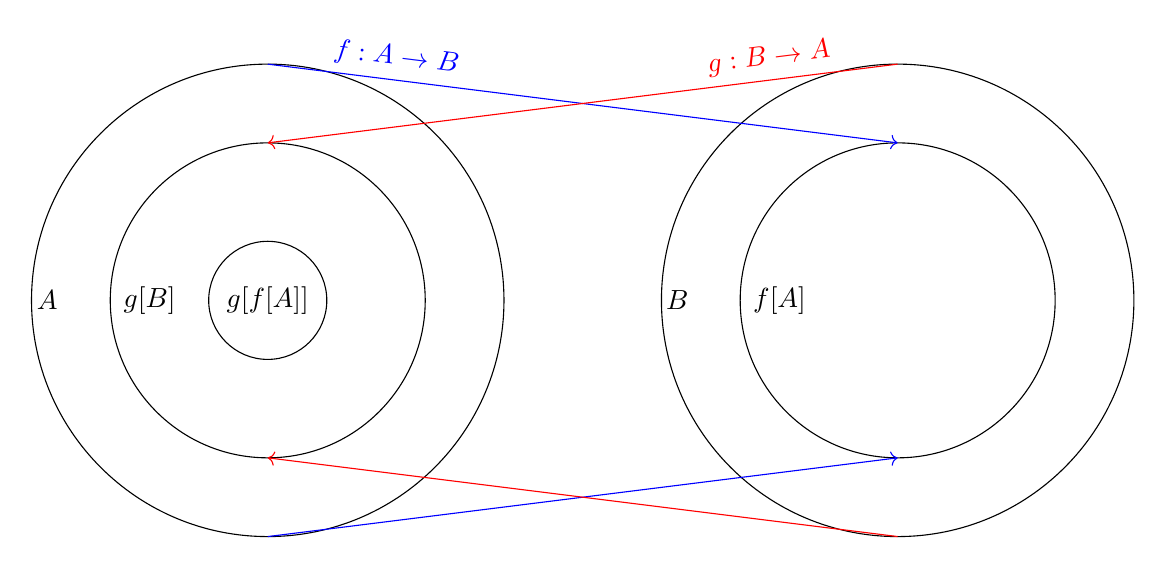
\begin{tikzpicture}
			\draw (-4, 0) circle (3); \draw (-6.8, 0) node {$A$};
			\draw (-4, 0) circle (2); \draw (-5.5, 0) node {$g[B]$};
			\draw (-4, 0) circle (0.75); \draw (-4, 0) node {$g[f[A]]$};
			
			\draw (4, 0) circle (3); \draw (1.2, 0) node {$B$};
			\draw (4, 0) circle (2); \draw (2.5, 0) node {$f[A]$};
			
			
			\draw[->, thin, blue] (-4, 3) -- (4, 2) node[pos=0.2, sloped, above, blue] {$f: A\to B$};
			\draw[->, thin, blue] (-4, -3) -- (4, -2);
			
			\draw[->, thin, red] (4, 3) -- (-4, 2)  node[pos=0.2, sloped, above, red] {$g:B\to A$};
			\draw[->, thin, red] (4, -3) -- (-4, -2);
			
		\end{tikzpicture}
	\end{center}
	\caption{Grafik des Sachverhalts im Satz \ref{SatzCantorSchroederBernstein}}
	\label{CantorSchroederBernsteinGrafik}
\end{figure}


\subsection{Ordinalzahlen}

Es wurden bereits die Zahlen $0,1,2,\dots,n,\dots,\omega,\omega+1,\omega+2,\dots,\omega+\omega$ diskutiert, mit welchen sich in diesem Kapitel genauer befasst werden soll.

Ein \textit{Graph} ist ein Paar $(A, R)$ so, dass $R\subseteq A\times A$ ein binäre Relation ist.

\begin{definition}[Partielle Ordnungen]
	Eine \textit{partielle Ordnung} ist ein Graph $(A,<)$ so, dass $<$ irreflexiv und transitiv ist. Eine alternative Definition ist $(A,\leq)$, wobei $\leq$ reflexiv, transitiv und antisymmetrisch ist.
\end{definition}

Eine \textit{lineare Ordnung} $(A,<)$ ist eine partielle Ordnung so, dass für alle $a,b\in A$ entweder $a<b$, $a=b$ oder $b<a$ gilt.

Ein Graph $(A,R)$ ist \textit{fundiert}, wenn jede nicht-leere Teilmenge $B\subseteq A$ ein Element $b\in B$ enthält so, dass $\{a\in B : (a,b) \in R\}= \emptyset$.
Also: Eine partielle Ordnung ist fundiert, wenn jede nicht-leere Teilmenge $B\subseteq A$ ein $<$-minimales Element enthält.

\begin{definition}[Wohlordnungen]
	Eine \textit{Wohlordnung} $(A,<)$ ist eine fundierte lineare Ordnung so, dass für jedes $a\in A$ die Klasse $\downarrow a\coloneqq \{b\in A : b < a\}$ eine Menge ist.
	Eine Relation $R\subseteq A\times A$, bei der für ein beliebiges $b$ die Klasse $\{a\in A : (a,b)\in R\}$ eine Menge ist wird auch als mengenähnlich bezeichnet.
\end{definition}

\begin{lemma}
	Sei $(A,<)$ eine fundierte, mengenähnliche, partielle Ordnung. Dann existiert in $A$ keine unendliche absteigende Folge $(a_n)_{n\in \omega}$ mit $a_{n+1}<a_n$ für alle $n$, wobei $\omega$ die Menge der natürlichen Zahlen bezeichnet.
\end{lemma}

Bemerkung: $(a_n)_{n\in \omega}$, $f:\omega \to A$ mit $a_n\coloneqq f(n)$

\begin{proof}
	Wenn eine solche Folge existiert, dann ist $\{a_n : n\in \omega\}=f[\omega]\subseteq A$ eine nicht-leere Klasse ohne $<$-minimales Element. Da $f[w]\subseteq \{a_0\}\cup \downarrow a$ und $A$ mengenähnlich ist, ist $f[w]$ eine Menge. Dies ist aber ein Widerspruch zur Fundiertheit.
\end{proof}

Um zu zeigen, dass jedes Element einer fundierten, mengenähnlichen partiellen Ordnung $(A,<)$ eine Eigenschaft $\psi$ erfüllt zeigt man, dass für für jedes $a$, dass wenn $\psi$ für alle $b<a$ gilt, dann auch für $a$.

\begin{satz}[Induktionsprinzip]
	Sei $(A,<)$ eine fundierte, mengenähnliche partielle Ordnung. Dann gilt
	\begin{itemize}
		\item[a)] Jede nicht-leere Klasse hat ein $<$-minimales Element.
		\item[b)] Sei $X\subseteq A$ so, dass für alle $a\in A$ gilt: Wenn $\downarrow a \subseteq X$, dann ist $a\in X$. Es folgt, dass $X=A$.
	\end{itemize}
\end{satz}
\begin{proof}
	a): Sei $B\subset A, a\in B$. Wegen der Mengenähnlichkeit ist $\downarrow a$ eine Menge und aus dem Aussonderungsaxiom folgt, dass auch $X\coloneqq B \cap (\downarrow a \cup \{a\})$ eine nicht-leere Teil\textit{menge} von $A$ ist. Es folgt auch, dass $X$ ein minimales Element $b$ besitzt. 
	
	Behauptung: $b$ ist auch das $<$-minimale Element von $B$. Andernfalls gibt es ein $c\in B$ mit $c < b \leq a$. Da $b\in X \subseteq B$ würde aber auch $c\in X$ folgen. Widerspruch!
	
	b): Annahme: $X$ sei wie gefordert, aber $X\neq A$. Also existiert ein $a\in A\setminus X$. Definiere $B\coloneqq \downarrow a \cup \{a\} \setminus \{X\}$. Dies ist eine nicht-leere Teilmenge und hat daher ein minimales Element $b$. Also ist $\downarrow b\subseteq A\setminus B\subseteq X$ und daher ist $b\in X$. Widerspruch!
\end{proof}

\begin{definition}[Ordinalzahlen]
	Eine \textit{Ordinalzahl} ist eine transitive Menge, welche durch $\in$ linear geordnet ist. 
	Beispiele sind $[n]$ für beliebige $n$, $\omega$, $\omega \cup \{\omega\}$. Die Klasse aller Ordinalzahlen ist $On$
\end{definition}

\begin{lemma}
	Ordinalzahlen sind wohlgeordnet durch $\in$.
\end{lemma}
\begin{proof}
	Sei $\beta\subseteq \alpha\in On$ und $\beta\neq \emptyset$. Da $\beta$ fundiert ist existiert ein $\gamma\in \beta$ mit $\gamma\cap \beta =\neq$. Also ist $\gamma$ kleinstes Element in $\beta$ bezüglich. $\in$
\end{proof}

\begin{definition}[Anfangsstück]
	Ein \textit{Anfangsstück} einer Ordnung $(A,<)$ ist eine Teilmenge $I\subseteq A$ so, dass, wenn $a\in I$ und $b<a$, auch $b\in I$ ist.
\end{definition}

Ein Anfangsstück von $\alpha \in On$ ist also eine Teilmenge $\beta\subseteq \alpha$ so, dass $\delta\in\gamma\in \beta\Rightarrow \delta\in\beta$, also eine transitive Teilmenge von $\alpha$.

\begin{lemma}
	Sei $\alpha\in On$. $\beta$ ist ein echtes Anfangsstück von $\alpha$, genau dann wen $\beta \in \alpha$
\end{lemma}
\begin{proof}
	\begin{itemize}
		\item[$\Rightarrow$:] Sei $\gamma$ das kleinste Element von $\alpha\setminus \beta$. 
		Es gilt $\beta=\gamma\in \alpha$, da für beliebige $\delta$ gilt, dass $\delta\in\gamma \Leftrightarrow (\delta\in\alpha \land \delta\notin\alpha\setminus\beta) \Leftrightarrow \delta\in\beta$
		\item[$\Leftarrow$:] Sei $\beta\in\alpha$ und $\delta\in\gamma\in\beta$. Es gilt $\delta\in\beta$, da sonst $\delta=\beta$ oder $\beta\in\delta$. Widerspruch!
	\end{itemize}
\end{proof}

\begin{satz}
	\begin{itemize}
		\item[a)] $(On,\in)$ ist ein Wohlordnung
		\item[b)] Wenn $\alpha\in On$, dann ist $\alpha=\{\beta\in On:\beta\in\alpha\}=\downarrow a$
		\item[c)] $On$ ist eine echte Klasse
	\end{itemize}
\end{satz}
\begin{proof}
	\begin{itemize}
		\item[a)] Zu zeigen ist, dass $\in$ eine lineare Ordnung ist. $\alpha \notin \alpha$ und $\alpha\in\beta, \beta\in \gamma\Rightarrow \alpha\in\gamma$ folgt direkt aus der Definition der Ordinalzahlen.
		
		Seien nun $\alpha,\beta\in On, \alpha\neq\beta$. Nun ist $x\in\alpha\cap\beta$ ein Anfangsstück von $\alpha$ und $\beta$. 
		Aus $y\in z \in \alpha\cap \beta$ folgt wegen der Transitivität $y\in\alpha\cap \beta$. Nun muss $x=\alpha$ oder $x=\beta$ gelten. Sonst ist $x\in \alpha$ und $x\in\beta$, also $\alpha\cap\beta \in \alpha\cap\beta$. Widerspruch!
		
		Wenn $x\in\alpha$, dann ist $x\in\beta$, also $\alpha \in \beta$, oder umgekehrt.
		
		\item[b)] Dies folgt direkt aus \textit{a)}
		
		\item[c)] Wäre $On$ eine Menge, wäre sie eine transitive, durch $\in$ linear geordnete Menge und müsste sich dadurch selbst enthalten. Widerspruch!
	\end{itemize}
\end{proof}

\begin{definition}[Nachfolgerordinal]
	Für $\alpha\in On$ ist $\alpha+1\coloneqq\alpha\cup \{\alpha\}$ das \textit{Nachfolgerordinal} von $\alpha$.
\end{definition}

\begin{definition}[Limesordinal]
	$\alpha\in On$ ist ein \textit{Limesordinal}, wenn $\alpha\neq\emptyset$ und $\alpha$ kein Nachfolgerordinal ist.
\end{definition}

Da $(On,\in)$, bzw. $(On,<)$, eine Wohlordnung ist, existiert die transfinite Induktion über $On$. Das heißt: für jede Teilklasse $X\subseteq On$ gilt: wenn für alle $\alpha\in On$ gilt, dass für jedes $\beta<\alpha$ aus $\beta\in X$ folgt, dass $\alpha\in X$, dann ist $X=On$.

Um zu zeigen, dass irgendeine Eigenschaft $\phi(x)$ auf alle Ordinale zutrifft, also $X\coloneqq\{\alpha\in On : \phi(x)\}=On$ gibt es folgende Strategien.
\begin{enumerate}
	\item Zeige, dass $\phi(0)$ gilt. Zeige, dass wenn $\phi(\alpha)$ auch $\phi(\alpha+1)$ ist. Zeige für jedes Limesordinal $\lambda$, dass $\phi(/lambda)$ gilt, wenn für alle $\alpha<\lambda$ auch $\phi(\alpha)$ korrekt ist.
	
	\item Betrachte eine beliebige Ordinalzahl $\alpha$ und nimm an, dass $\phi(\beta)$ für alle $\beta<\alpha$ gilt. Zeige, dass dann $\phi(\alpha)$ folgt.
\end{enumerate}

\subsubsection{Ordinale und Stufen}

Zur Erinnerung: für jede Menge $a$ ist $S(a)$ die kleinste Stufe mit $a\subseteq S(a)$ und aus $a\in b$ folgt $S(a)\in S(b)$.

Letzteres gilt natürlich auch für Ordinalzahlen. Wir wollen nun aber auch die Umkehrung betrachten. Wenn $\alpha\notin\beta$ ist, dann folgt $\alpha=\beta$ oder $\beta\in\alpha$, also $S(\alpha)=S(\beta)$ oder $S(\beta)\in S(\alpha)$. In beiden Fällen gilt $S(\alpha)\notin S(\beta)$. Es gilt also auch die Rückrichtung: $\alpha\in\beta \Leftrightarrow S(\alpha)\in S(\beta)$.

\begin{satz}
	Die Funktion $F:On \to H(\mathcal{S}), F(\alpha)\coloneqq S(\alpha)$ ist ein Isomorphismus zwischen $On$ und $H(\mathcal{S})$. Das heißt $F$ ist bijektiv und $\beta<\alpha \Leftrightarrow F(\beta)\in F(\alpha)$.
\end{satz}

Bemerkung: Mit $H(\mathcal{S})$ wird die Klasse aller Stufen, die Mengen sind, also aller Stufen außer $\mathcal{S}$ bezeichnet.

\begin{proof}
	Es ist bereits bekannt, dass $F$ injektiv und ein starker Homomorphismus ist. Es bleibt die Surjektivität zu beweisen. Wenn dies nicht der Fall wäre, dann existierte eine minimale Stufe $S\in\mathcal{S}$ mit $S\notin Bild(F)$. 
	
	Sei $X\coloneqq\{\beta\in On:S(\beta)\in S\}$. $X$ ist ein echtes Anfangsstück von $On$, das heißt es gibt $\alpha\in On$ so, dass $X=\downarrow \alpha=\alpha$. Demnach betrachten wir nun $S(\alpha)$ und wie sich dies zu $S$ verhält.
	\begin{itemize}
		\item $S(\alpha)\in S$, dann ist $\alpha\in X=\alpha$. Widerspruch!
		\item $S(\alpha)=S$, dann ist $S\in Bild(F)$. Widerspruch!
		\item $S\in S(\alpha)$, dann ist $S(\alpha)$ die kleinste Stufe so, dass $\alpha\subseteq S(\alpha)$, sodass $\beta\in S(\alpha)$ für alle $\beta\in\alpha$ gilt. 
		Da aber $\beta\in S(\beta)\in S$ für alle $\beta\in\alpha$ ist, folgt $S(\alpha)\subseteq S$. Widerspruch!
	\end{itemize}
\end{proof}

\begin{definition}
	Für $\alpha\in On$, setze $S_\alpha\coloneqq S(\alpha)$. Dies sind dann die \textit{Indices der kumulativen Hierarchie}.
\end{definition}

Es folgt, dass $S_0\subset S_1 \subset \dots \subset S_\omega \subset \dots \subset S_\alpha \subset S_{\alpha+1}\subset\dots$, $H(\mathcal{S})=\{S_\alpha:\alpha\in On\}$ und $\mathcal{S}=\bigcup\{S_\alpha : \alpha\in On\}$.

\begin{definition}[Rang einer Menge]
	Der \textit{Rang} einer Menge $a$ ist das Ordinal $\rho(a)=\alpha$ mit $S(a)=S_\alpha$.
\end{definition}

Für Ordinale $\alpha$ gilt $\rho(\alpha)=\alpha$. Eine Klasse $X$ ist eine Menge genau dann, wenn $\{\rho(x):x\in X\}$ durch eine Ordinalzahl beschränkt ist.

\subsubsection{Der Rekursionssatz}

Sei $A$ eine Klasse und definiere $A^\infty\coloneqq\{f : f:\alpha\to A, \text{Fkt. für ein} \alpha\in On\}$. Dies lässt sich in Worten als die Menge aller Folgern der Länge $\alpha$.

Sei $G$ nun eine partielle Funktion $G:\mathcal{S}^\infty\to\mathcal{S}$.

\begin{lemma}
	Es gibt höchstens eine Funktion $f:\alpha\to \mathcal{S}$ so, dass $f$ eine Menge ist und $f(\beta)=G(f\upharpoonright\beta)$ für alle $\beta < \alpha$.
\end{lemma}
Bsp.: $f(17)=G(f\upharpoonright\{0,\dots,16\})$.
\begin{proof}
	Nehmen wir an, dass $f$ und $f'$ die geforderte Eigenschaft erfüllen. Sei $X=\{\beta \in\alpha : f(\beta)=f'(\beta)\}$. Wenn $\beta < \alpha$ und $\beta\subseteq X$, dann $f\upharpoonright\beta =f'\upharpoonright\beta$, also $f(\beta)=G(f\upharpoonright\beta)=G(f'\upharpoonright\beta)=f'(\beta)$, also $\beta\in X$. Es folgt $X=\alpha$ und $f=f'$.
\end{proof}

Nun ist das Ziel zu zeigen, dass jede totale Funktion $G:\mathcal{S}^\infty\to\mathcal{S}$ auf eindeutige Weise eine Funktion $F:On\to\mathcal{S}$ definiert.

Für die Existenz wird aber ein zusätzliches Axiom benötigt:

\textit{Ersetzungsaxiom}: Wenn $F:A\to S$ eine Funktion ist und $a\subseteq A$ eine Menge ist, dann ist auch $F[a]$ eine Menge. Oder in anderen Worten: Wenn $F$ eine Funktion ist und $Def(F)$ eine Menge ist, dann ist auch $Bild(F)$ eine Menge.

\begin{satz}[Rekursionssatz]
	Zu jeder Funktion $G:\mathcal{S}^\infty\to\mathcal{S}$ gibt es genau eine Funktion $F:On\to\mathcal{S}$ so, dass $F(\alpha)=G(F\upharpoonright\alpha)$ für alle $\alpha\in On$.
\end{satz}
\begin{proof}
	Sei $\alpha\in On$. Wir wissen dass es höchstens eine Funktion $f_\alpha:\alpha\to\mathcal{S}$ mit $f_\alpha(\beta)=G(f\alpha\upharpoonright\beta)$ für alle $\beta<\alpha$ gibt.
	
	Die Existenz solch einer Funktion $f_\alpha$ soll nun per Induktion nach $\alpha$ geschehen so, dass für alle $\beta<\alpha$ gilt, dass $f_\beta=f_\alpha\upharpoonright\beta$.
	
	$\alpha=0$: Dann ist $f_\alpha=\emptyset$, die Bedingung gilt also.
	
	$\alpha+1$: Dann lässt sich $f_{\alpha+1}$ als $f_{\alpha+1}\coloneqq f_\alpha\cup\{(\alpha, F(f_\alpha))\}$ definieren.
	
	Sei $\alpha$ ein Limesordinal. Setze $X\coloneqq\{f_\beta : \beta < \alpha\}$. $X$ ist eine Menge, denn $X$ ist das Bild der Funktion $H:\alpha\to\mathcal{S}^\infty$ mit $H(\beta)=f_\beta$ für $\beta\in\alpha$.
	
	Nun ist $f_\alpha\coloneqq\bigcup X=\{(\gamma,f_\beta(\gamma), \gamma<\beta<\alpha)\}$. $f_\alpha$ ist tatsächlich eine Funktion von $\alpha$ nach $\mathcal{S}$: Für alle $\gamma<\alpha$ existiert ein $\beta$ mit $\gamma<\beta<\alpha$ und damit ein Paar $(\gamma,f_\beta(\gamma))\in f_\alpha$. Für $(\gamma,f_\beta(\gamma)),(\gamma,f_{\beta'}(\gamma))\in f_\alpha$ so, dass $\beta<\beta'$ ist $f_\beta=f_{\beta'}\upharpoonright \beta$, also $f_\beta(\gamma)=f_{\gamma'}(\gamma)$. Es folgt also $Def(f_\alpha)=\alpha$.
	
	Setze $F=\bigcup\{f_\alpha:\alpha\to\mathcal{S} : \alpha\in On\}$. $F=\{(\beta, f_\alpha(\beta)):\beta<\alpha\in On\}$, $F$ ist eine Funktion mit $Def(F)=On$.
	
	Für jedes $\beta\in On$ ist $F(\beta)=f_\alpha(\beta)$ für ein (und damit alle!) $\alpha$ mit $\beta<\alpha$.
	
	$F\upharpoonright\beta=f_\alpha\upharpoonright\beta$ für $\beta<\alpha$, $F(\beta)=f_\alpha(\beta)=G(f_\alpha\upharpoonright\beta)=G(F\upharpoonright\beta)$.
\end{proof}

Damit ist der Rekursionssatz bewiesen. Nun sollen Anwendungen von diesem gezeigt werden.\\

\textit{Konstruktion von $F:On\to A$}: Sei $a\in A,s:A\to A, h: \Pot{A}\to A$. Nun lässt sich $G:A^\infty\to A$ definieren durch: $G(\emptyset)\coloneqq a, G(F\upharpoonright\alpha+1)\coloneqq s(F(\alpha)), G(F\upharpoonright\lambda)\coloneqq h(F[\lambda])$ für ein Limesordinal $\lambda$ und Nachfolgerordinal $\alpha$.

Mit dem Rekursionssatz folgt die Existenz und Eindeutigkeit der Funktion $F:On\to A$ mit $F(\alpha)=F(F\upharpoonright\alpha)$. Es gilt $F(\emptyset)=a, F(\alpha+1)=s(F(\alpha)), F(\lambda)=h(F[\lambda])$.\\

\textit{Addition von Ordinalzahlen}: Es sollen nun Ausdrücke wie $\alpha+\beta$ definiert werden, für $\alpha,\beta\in On$. $\alpha+\beta\coloneqq F_\alpha:On\to On, \beta\mapsto\alpha+\beta$. 
Genauer lässt sich rekursiv definieren, dass 
\begin{align*}
	&\alpha+0\coloneqq\alpha,\\
	&\alpha+(\beta+1)\coloneqq(\alpha+\beta)+1,\\ 
	&\alpha+\lambda\coloneqq\sup\{\alpha+\beta : \beta < \lambda\}
\end{align*}
für ein Limesordinal $\lambda$.

\textit{Bemerkung}: Addition ist nicht kommutativ! Dies lässt sich leicht an einem Beispiel erkennen: $\omega+1=\omega\cup\{\omega\}\neq\omega$, aber $1+\omega=\sup\{1+n:n\in\omega\}=\omega$.

Eine andere interessante Beobachtung ist, dass sich Addition zweier Ordinalzahlen durch \glqq Hintereinanderlegen\grqq{} zweier Wohlordnungen darstellen lässt. Für $\alpha+\beta$ lassen sich Strukturen $\mathfrak{A}=(A,<), \mathfrak{B}=(B,<)$ finden, wobei beide Strukturen Wohlordnungen sind. Das \glqq Hintereinanderlegen\grqq{} lässt sich in Abbildung \ref{AdditionWO} erkennen. Da $\mathfrak{A}$ und $\mathfrak{B}$ beides Wohlordnungen sind, lässt sich leicht einsehen, dass dann auch $\mathfrak{A}+\mathfrak{B}$ eine Wohlordnung ist.
	
\begin{figure}[h]
	\begin{center}
		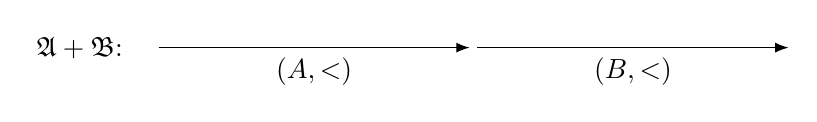
\begin{tikzpicture}
			\draw (-5, 0) node {$\mathfrak{A}+\mathfrak{B}$:};
	
			\draw[-{Latex}, thin] (-4, 0) -- (-0.05, 0) node[midway, below] {$(A,<)$};		
			\draw[-{Latex}, thin] (0.05, 0) -- (4, 0) node[midway, below] {$(B,<)$};
		\end{tikzpicture}
	\end{center}
	\caption{Darstellung von Addition durch \glqq Hintereinanderlegen\grqq{} von Wohlordnungen}
	\label{AdditionWO}
\end{figure}

\textit{Multiplikation von Ordinalzahlen}: Analog zur Addition kann man auch die Multiplikation definieren. Für $\alpha,\beta\in On$ ist dafür definiert:
\begin{align*}
	&\alpha\cdot0\coloneqq 0\\
	&\alpha\cdot(\beta+1)\coloneqq\alpha\cdot\beta+\alpha\\
	&\alpha\cdot\lambda\coloneqq\sup\{\alpha\cdot\beta : \beta<\lambda\}
\end{align*}
für ein Limesordinal $\lambda$.

Und ebenso, wie Addition durch Wohlordnungen darstellbar ist, lässt sich Multiplikation mithilfe von zwei Wohlordnungen $\mathfrak{A}=(A,<)$ und $\mathfrak{B}=(B,<)$ bilden. Dabei gilt $\mathfrak{A}\cdot\mathfrak{B}\coloneqq\mathfrak{C}=(A\times B, <_C)$ mit $(a,b)<_C(a',b')$ genau dann, wenn $b<b'$ oder $b=b'\land a<a'$. Graphisch dargestellt ist dies in Abbildung \ref{MultiplikationWO}.
	
\begin{figure}[h]
	\begin{center}
		\begin{tikzpicture}
			\draw[-{Latex}, thin] (-5, 0) -- (-1, 0) node[midway, below] {$\mathfrak{A}$};
			
			\draw (-0.5, 0) node[very thick] {$\cdot$};
			
			\draw[-{Latex}, thin] (0, -2) -- (0, 2) node[midway, right] {$\mathfrak{B}$};
			
			\draw (1, 0) node[very thick] {$=$};
			
			\draw[-{Latex}, thin] (1.5, -2) -- (1.5, 2);
			
			% Top (y=2)
			\draw[-{Latex}, thin] (1.7, 1.7) -- (5.7, 1.7);
			
			% Upper (y=1)
			\draw[-{Latex}, thin] (1.7, 0.85) -- (5.7, 0.85);
			
			% Middle (y=0)
			\draw (3.7, 0) node[very thick] {$\vdots$};
			
			% Lower (y=-1)
			\draw[-{Latex}, thin] (1.7, -0.85) -- (5.7, -0.85);
			
			% Bottom (y=-2)
			\draw[-{Latex}, thin] (1.7, -1.7) -- (5.7, -1.7);
			
		\end{tikzpicture}
	\end{center}
	\caption{Graphische Darstellung von Multiplikation mithilfe von Wohlordnungen}
	\label{MultiplikationWO}
\end{figure}

Auch hier lässt es sich wieder feststellen, dass Multiplikation nicht kommutativ ist. Ein Beispiel hierfür ist $\omega\cdot 2=\omega\cdot(1+1)=\omega+\omega=\sup\{\omega+n : n\in\omega\}>\omega+n$ für alle $n\in\omega$, aber $2\cdot\omega=\sup\{2\cdot n : n<\omega\}=\omega<\omega+1$.

Also gilt im Allgemeinen auch \textbf{nicht} $(\alpha+\alpha')\cdot\beta=\alpha\beta+\alpha'\beta$, da beispielsweise $(1+1)\cdot\omega=2\cdot\omega=\omega \neq \omega+\omega = 1\cdot\omega+1\cdot\omega$.\\

\textit{Potenzen von Ordinalzahlen}: Zuletzt wird nun noch das Potenzieren von Ordinalzahlen definiert. Für $\alpha,\beta,\lambda\in On$, $\alpha, \beta$ Nachfolgerordinale und $\lambda$ ein Limesordinal sein nun definiert:
\begin{align*}
	&\alpha^0\coloneqq1\\
	&\alpha^{\beta+1}\coloneqq\alpha^\beta\cdot\alpha\\
	&\alpha^\lambda\coloneqq\sup\{\alpha^\beta:\beta<\lambda\}.
\end{align*}

\begin{satz}[Cantor-Normalform]
	Jedes $\alpha\in On$ hat eine eindeutige Darstellung $\alpha=\omega^{\beta_1}\cdot n_1+\dots+\omega^{\beta_k}\cdot n_k$ mit $k\in\omega, n_1,\dots, n_k\in\omega\setminus\{0\}$ und $\alpha\geq\beta_1>\beta_2>\dots>\beta_k\geq0$.
\end{satz}
\begin{proof}
	Dies soll per Induktion gezeigt werden. Für $\alpha=0$ ist dies trivial, da dies die einzige Darstellung der $0$ ist. Sei unsere Induktionsvoraussetzung nun also, dass alle Ordinale, die kleiner als $\alpha$ sind eine eindeutige Cantor-NF besitzen.
	
	Sei $\gamma$ das kleinste Ordinal so, dass $\omega^\gamma>\alpha$. $\gamma$ muss ein Nachfolger sein, denn wäre es ein Limesordinal, dann wäre $\gamma$ nicht das kleinste Ordinal mit der geforderten Eigenschaft.
	
	Also ist $\gamma=\beta+1$ und $\beta$ ist das größte Ordinal mit $\omega^\beta \leq \alpha$. Also existieren Ordinale $n<\omega$ und $\gamma$ so, dass $\alpha=\omega^\beta\cdot n+\gamma, \gamma<\omega^\beta\leq\alpha$.
	
	Nach der Induktionsvoraussetzung hat $\gamma$ eine eindeutige Cantor-Normalform und damit auch $\alpha$.
\end{proof}

Es lässt sich jedoch feststellen, dass die Cantor-NF nicht immer hilfreich ist. Sei beispielsweise $\omega_1=\min\{\alpha\in On : \text{ es gibt keine injektive Abb.} f:\alpha\to\omega\}$ das kleinste nicht abzählbare Ordinal. Gesucht sei nun die Cantor-Normalform von $\omega_1$.

$\omega_1=\sup\{\alpha\in On : \alpha \text{ ist abzählbar}\}$ ist ein Limesordinal. Betrachte nun $\omega^{\omega_1}=\sup\{\omega^\alpha : \alpha \text{ ist abzählbar}\}$. Es lässt sich feststellen, dass $\omega^{\omega_1}\leq\omega_1\leq\omega^{\omega_1}$, also muss $\omega_1=\omega^{\omega_1}$ sein.

Die Cantor-NF von $\omega_1$ ist also $\omega^{\omega_1}$, was offensichtlicherweise nicht sonderlich hilfreich ist.

\begin{satz}[Ordinale Normalform für Wohlordnungen]
	Jede Wohlordnung $(a,<)$ über einer Menge $a$ ist isomorph zu genau einer Ordinalzahl.
\end{satz}
\begin{proof}
	Zu einer gegebenen Wohlordnung $(a,<)$ suchen wir ein $\alpha\in On$ und eine bijektive Abbildung $f:\alpha\to a$ so, dass für $\gamma<\beta<\alpha$ auch $f(\gamma)<f(\beta)$ ist.
	
	Definiere $F:On\to a\cup\{a\}$ durch
	$$
	F(\alpha)\coloneqq\begin{cases}
		\min\{a\setminus F[\alpha]\} & \text{wenn } F[\alpha]\subsetneqq a\\
		a & \text{sonst}
	\end{cases}
	$$
	
	Behauptung: $a\in Bild(F)$. Andernfalls wäre $F$ eine injektive Abbildung von $On$ nach $a$, dann wäre für $\beta<\alpha$ aber entweder $F(\alpha)\notin F[\alpha]$ oder $F(\beta)\in F[\alpha]$, also $F(a)\neq F(b)$. Das heißt, dass $F:On\to Bild(F)$ bijektiv ist und da $Bild(F)\subseteq a$ eine Menge ist, müsste $F^{-1}[Bild(F)]=On$ nach dem Ersetzungsaxiom eine Menge sein. Widerspruch!
	
	Sei $\alpha$ also die kleinste Ordinalzahl so, dass $F(\alpha)=a$. Dann ist $f:F\upharpoonright \alpha$ die gesuchte Bijektion:
	\begin{itemize}
		\item $f$ ist Ordnungserhaltend und damit auch injektiv, da für $\gamma<\beta<\alpha$ folgt, dass $f[\gamma]\subsetneqq f[\beta]$, da $f(\gamma)=\min\{a\setminus f[\gamma]\}<\min\{a\setminus f[\beta]\}=f(\beta)$.
		\item $f$ ist surjektiv, da sonst ein kleinstes Element $b\in a\setminus f[\alpha]$ existieren würde. Dann wäre $F(\alpha)=b$ im Widerspruch zu $F(\alpha)=a$.
	\end{itemize}
\end{proof}

\subsection{Das Auswahlaxiom (AC)}

\begin{definition}[Auswahlfunktionen]
	Eine \textit{Auswahlfunktion} auf einer Menge $x$ ist eine Funktion $f:x\to\mathcal{S}$ so, dass $f(z)\in z$ für jedes nicht-leere $z\in x$.
\end{definition}

Das Auswahlaxiom (AC) besagt, dass auf jeder Menge eine solche Auswahlfunktion existiert.\\

Es lässt sich sehen, dass wenn auf $\bigcup X$ eine Wohlordnung existiert, man eine Auswahlfunktion bilden kann, ohne das Auswahlaxiom nutzen zu müssen. Sei $z\in x, z\neq\emptyset$. Dann ist $f(z)=\min(z)$ eine Auswahlfunktion. 

Dies ist die eine Richtung des Wohlordnungssatzes von Zermelo, welches auch aus dem AC folgt. Die andere Richtung soll nun ebenfalls gezeigt werden.

\begin{satz}[Wohlordnungssatz von Zermelo]
	Auf jeder Menge $a$ existiert eine Wohlordnung.
\end{satz}
\begin{proof}
	Aus einer Auswahlfunktion $f$ auf $\Pot{a}$ können wir eine Wohlordnung auf $a$ konstruieren. Sei $F:On\to a\cup \{a\}$ mit
	$$
	F(\alpha)=\begin{cases}
		f(a\setminus F[\alpha]) & \text{wenn } F[\alpha]\subsetneqq a \\
		a & \text{sonst}
	\end{cases}
	$$
	Wie im letzten Beweis gezeigt gibt es ein $\alpha\in On$ mit $F(\alpha)=a$ und $F\upharpoonright \alpha:\alpha\to a$ bijektiv.
	
	$F\upharpoonright\alpha$ ist surjektiv, denn sonst ist $F(\alpha)\neq a$ und $F\upharpoonright\alpha$ überträgt de Wohlordnung von $\alpha$ auf $a$. Für $y,z\in a$ setze $y <_a z$ genau dann, wenn $(F\upharpoonright\alpha)^{-1}(y) < (F\upharpoonright\alpha)^{-1}(z)$.
\end{proof}

Ein weiteres, zum Auswahlaxiom äquivalentes Axiom ist das Lemma von Zorn (Kuratowski).
Dieses besagt, dass wenn $(a,<)$ eine partielle Ordnung auf einer Menge $a$ ist, in der jede linear geordnete Teilmenge $b\subseteq a$ eine obere Schranke $s_b\in a$ hat, die Menge ein maximales (bemerke: nicht größtes) Element $m_a$ besitzt.

\begin{satz}
	Aus den Axiomen von ZF und dem Auswahlaxiom lässt sich das Lemma von Zorn folgern.
\end{satz}
\begin{proof}
	Sei $f$ eine Auswahlfunktion auf $\Pot(a)$. Für jede Teilmenge $b\subseteq a$, welche durch $<$ linear geordnet ist, setze $y_b\coloneqq\{x\in a:\forall u(u\in b\rightarrow u<x)\}$ als die Menge der \textit{echten} oberen Schranken von $b$.
	
	Definiere nun $F:\Pot{a}\to a\cup\{a\}$ durch
	$$
	F(b)\coloneqq\begin{cases}
		f(y_b) & \text{wenn } b \text{ durch } < \text{ linear geordnet ist und } y_b\neq\emptyset \\
		a & \text{sonst}
	\end{cases}
	$$
	
	Mithilfe des Rekursionssatzes lässt sich dann eine Funktion $G: On\to a\cup\{a\}$ mit $\alpha\mapsto G(G[\alpha])=F(Bild(G\upharpoonright\alpha))$ definieren.
	
	$G[\alpha]$ ist eine linear geordnete Teilmenge von $a$ und $G(\alpha)$ ist eine echte obere Schranke für $G[\alpha]$ außer dann, wenn $G[\alpha]$ keine echte obere Schranke besitzt, dann gilt $G(\alpha)=a$.
	
	Wie in vorherigen Beweisen folgt, dass $G$ den Wert $a$ annehmen muss, da sonst $G$ eine ordnungserhaltende Abbildung von $On$ nach $a$ wäre und $On$ eine Menge sein würde.
	
	Sei $\alpha$ also minimal mit $G(\alpha)=a$. $G[\alpha]$ ist nach Konstruktion eine linear geordnete Teilmenge von $a$ ohne \textit{echte} obere Schranke.
	
	Sei $m$ eine obere Schranke (und damit größtes Element) von $G[\alpha]$. Damit ist $m$ maximales Element von $(a,y)$.
\end{proof}

\begin{satz}
	Aus den Axiomen von ZF und dem Lemma von Zorn folgt das Auswahlaxiom.
\end{satz}
\begin{proof}
	Sei $x$ eine beliebige Menge und $a\coloneqq\{f:z\to\bigcup z : z\subseteq x \text{ und } f \text{ ist eine Auswahlfunktion auf } z\}$.
	Es gilt $a\neq\emptyset$, da die leere Funktion in $a$ ist und $a$ ist durch $\subsetneqq$ partiell geordnet.
	
	Wir behaupten, dass jede lineare geordnete Teilmenge $b\subseteq a$ eine obere Schranke $g_b\in a$ besitzt. Setze $g_b\coloneqq \bigcup b\subseteq x\times \bigcup x$, so dass $g_b=\{(c, f(c)) : c\in z\subseteq x, f:z\to\bigcup z, f\in b\}$. Wenn $(c,f(c)),(c,f'(c))\in g_b$ sind, dann ist $f, f'\in b$, aber es gilt $f\subseteq f'$ oder $f'\subseteq f$. Da $f,f'$ Funktionen sind, folgt $f(c)=f'(c)$, $g_b$ ist also eine wohldefinierte Funktion.
	
	Für $c\in Def(g_b)$ ist $g_b(c)=f(c)\in c$ für ein $f\in b$. Also ist $g_b$ eine Auswahlfunktion, das heißt $g_b\in a$.
	
	Schließlich ist $g_b$ eine obere Schranke für $b$, also besitzt $a$ nach dem Zornschen Lemma ein maximales Element $f\in a$.
	
	Behauptung: $f$ ist eine Auswahlfunktion auf $x$. Wenn nicht, dann ist $f$ eine Auswahlfunktion auf einer echten Teilmenge $z\subsetneqq x$ und es gibt ein nicht-leeres $y\in x\setminus z$. Für jedes $c\in y$ ist dann $f'\coloneqq f\cup\{(y,c)\}$ eine Auswahlfunktion auf $z\cup\{y\}\subseteq x$ mit $f\subsetneqq f'$. Widerspruch zur Maximalität von $f$.
\end{proof}

\subsubsection{Folgerungen aus dem Auswahlaxiom}

\begin{satz}
	Jeder Vektorraum hat eine Basis.
\end{satz}
\begin{proof}
	Sei $V$ ein Vektorraum. Wenn $V=\{0\}$, dann ist $\emptyset$ eine Basis. Sei also $V\neq\{0\}$. Definiere $X\coloneqq\{B\subseteq V : B\text{ ist unabhängig}\}$ (zur Erinnerung: $B\subseteq B$ ist unabhängig, wenn kein Element $v\in B$ sich als endliche Linearkombination von anderen Elementen aus $B$ schreiben lässt).
	
	$X$ ist nicht leer, da für $V\neq\{0\}, v\in V$ die Menge $\{v\}$ linear unabhängig ist.
	
	Weiter folgt, dass $(X,\subsetneqq)$ eine partielle Ordnung ist, in der jede Kette $K\subseteq X$ eine obere Schranke, nämlich $\bigcup K$ besitzt. Es gilt $\bigcup K\in X$, denn sonst lässt sich ein $v\in\bigcup K$ als endliche Linearkombination $v=\lambda_1v_1+\dots+\lambda_kv_k$ schreiben. Aber dann existiert ein $B\in K$ mit $v,v_1,\dots,v_m\in B$.
	
	Nach dem Lemma von Zorn hat $X$ also ein maximales Element $B_{max}$. $B_{max}$ ist unabhängig, jedes $v\in V$ lässt sich als Linearkombination $v=\lambda_1v_1+\dots+\lambda_mv_m$ schreiben. Sonst wäre $B_\{max\}\bigcup \{v\}$ unabhängig, im Widerspruch zur Maximalität von $B_{max}$.
\end{proof}

Eine weitere Folgerung des Auswahlaxioms ist der Satz von Banach-Tarski, welcher im folgenden Kapitel genauer betrachtet werden soll.

\subsubsection{Der Satz von Banach-Tarski}

Informell lässt sich der Satz wie folgt definieren: \glqq Eine Kugel $B\subseteq\mathbb{R}^3$ kann in endlich viele Teile zerlegt werden, die dann via einfacher Isometrien zu zwei disjunkten Kopien von $B$ zusammengesetzt werden können.\grqq{}

Im Folgenden werden nun einige begriffe definiert:

\begin{definition}[Isometrie]
	Sei $A\subseteq\mathbb{R}^3$. Eine Funktion $\phi:A\to\mathbb{R}^3$ ist eine \textit{Isometrie}, wenn $\Vert\phi(a)-\phi(b)\Vert=\Vert a-b\Vert$ für alle $a,b\in A$.
\end{definition}

\begin{definition}[Kongruenz]
	Zwei Mengen $A,B\subseteq\mathbb{R}^3$ sind \textit{kongruent} ($A\cong B$), wenn eine Isometrie $\varphi$ auf $A$ existiert mit $\varphi(A)=B$.
\end{definition}

\begin{definition}[Zerlegungsäquivalenz]
	$A, B$ sind \textit{Zerlegungsäquivalent} ($A\sim_z B$), wenn $n\in\mathbb{N}$ und Partitionen $A=A_1\cup\dots\cup A_n, B=B_1\cup\dots\cup B_n$ existieren, mit $A_i\cong B_i$ für alle $i\leq n$.
\end{definition}

Es bleibt nun zu zeigen, dass $\sim_z$ eine Äquivalenzrelation ist. Reflexivität und Symmetrie ist leicht einsehbar, gezeigt werden muss nun also nur noch die Transitivität.

Sei $A\sim_z B$ und $B\sim_z C$. Es gibt also Partitionen 
\begin{align*}
	&A=A_1\cup\dots\cup A_n,\\
	&B=B_1\cup\dots\cup B_n \text{ mit}\\
	&\varphi_i \text{ so, dass q} A_i\cong B_i, \forall i\leq n
\end{align*}
und 
\begin{align*}
	&B=B'_1\cup\dots\cup B'_m,\\
	&C=C_1\cup\dots\cup C_m \text{ mit}\\
	&\psi_i \text{ so, dass } B'_i\cong C_i, \forall i\leq m
\end{align*}

Setze $B_{ij}\coloneqq B_i\cap B'_j, i\leq n, j\leq m$, wodurch wieder eine Partition von $B$ gebildet wird. Weiter sei $A_{ij}\coloneqq\phi_i^{-1}(B_{ij})$ und $C_{ij}\coloneqq\psi_j(B_{ij})$.

Dann ist $\psi_j\circ\phi_i$ eine Isometrie von $A_{ij}$ nach $C_{ij}$ und $A_{ij}, C_{ij}$ bilden Partitionen von $A$ bzw. $C$, also ist $A\sim_z C$.

Weiter kann man folgende Eigenschaften der Relationen $\sim_z$ feststellen, welche hier aber nicht bewiesen werden sollen:
\begin{itemize}
	\item Wenn $A\sim_z B$, dann existiert eine Bijektion $g:A\to B$ mit $C\sim_z g(C)$ für alle $C\subseteq A$
	\item Für Partitionen $A=A_1\cup\dots\cup A_n, B=B_1\cup\dots\cup B_n$ mit $A_i\sim_z B_i$ folgt $A\sim_z B$.
	\item Wir definieren $A\leq B\colon\Leftrightarrow \exists B'\subseteq B : A\sim_z B'$
	\item Wenn $A\leq B$ und $B\leq A$, dann ist $A\sim_z B$
\end{itemize}

Ein Vorbereitender Satz für den Satz von Banach-Tarski ist das Hausdorff-Paradoxon. Dieses beschreibt eine Paradoxe Zerlegung der $2-$Sphäre $S^2=\{(x,y,z)\in\mathbb{R}^3 : x^2+y^2+z^2=1\}$.

\begin{satz}[Hausdorff-Paradoxon]
	Es gibt Mengen $A,B,C,D\subseteq S^2$ mit
	\begin{itemize}
		\item $A,B,C,D$ bilden eine Partition von $S^2$
		\item $D$ ist abzählbar
		\item $A\cong B \cong C \cong (B\cup C)$
	\end{itemize}
\end{satz}
\begin{proof}
	Definiere
	$$
	\psi\coloneqq
	\begin{pmatrix}
		-\frac{1}{2} & \frac{\sqrt{3}}{2} & 0 \\
		-\frac{\sqrt{3}}{2} & -\frac{1}{2} & 0 \\
		0 & 0 & 1 \\
	\end{pmatrix}
	$$
	als eine Rotation um $\frac{2\pi}{3}=120^\circ$, um die z-Achse (die z-Achse ist die Achse, die nach \glqq oben\grqq{} geht). Es gilt $\psi^3=1=id_{\mathbb{R}^3}$.
		
	Weiter sei 
	$$
	\varphi_\theta\coloneqq
	\begin{pmatrix}
		-\cos \theta & 0 & \sin \theta \\
		0 & -1 & 0 \\
		\sin \theta & 0 & \cos \theta 
	\end{pmatrix}
	$$
	eine Rotation um $\pi=180^\circ$, um die Achse $a_\theta$ in der x-z-Ebene (die x-z-Ebene ist die Ebene parallel zur Tafel in der Vorlesung). Hier gilt dann $\varphi_\theta\cdot\varphi_\theta=1$.
	
	Die Gruppe $(G_\theta, \cdot)$ lässt sich nun durch reduzierte Wörter $g=g_1\dots g_n$ über dem Alphabet $\Gamma=\{\psi, \psi^2,\phi\}$ darstellen so, dass hintereinander stehende Zeichen, welche sich zu $1$ kürzen nicht vorkommen. Die Darstellung ist also eindeutig.
	
	Wir wollen $\theta$ so wählen, dass $G_\theta$ frei ist, das heißt, dass für jedes $g\in G_\theta$ genau eine Darstellung $g=g_1\dots g_n$ durch ein reduziertes Wort existiert. Solche $\theta$ existieren.
	
	Für $g=g_1\dots g_n\in \Gamma^\ast$ sei $g(\theta)$ die Rotation die entsteht, wenn wir $\varphi=\varphi_\theta$ setzen. Und es sei $\theta_g\coloneqq\{\theta\in[0,2\pi) : g(\theta)=1\}$.
	
	\begin{lemma}
		Für jedes $g\in\Gamma^\ast\setminus\{\varepsilon\}$ ist $\theta_g$ endlich.
		\label{HausdorffOhneProof}
	\end{lemma}

	Mithilfe des Lemmas \ref{HausdorffOhneProof} lässt sich folgern, dass $M=\bigcup\limits_{g\in\Gamma^+, g\text{ red.}}\theta_g$ abzählbar ist und wir ein $\theta\in [0,2\pi]\setminus M$ finden können. Dann ist $g(\theta)\neq 1$ für alle reduzierten $g\in\Gamma^+$ und also $G_\theta$ frei über $\{\psi,\psi^2,\varphi_\theta\}$. Fixiere ein solches $\theta$ und sei $\varphi\coloneqq\varphi_\theta$ sowie $D\coloneqq\{s\in S^2 : gx=x\text{ für ein } g\in G_\theta\}$. Jede nicht-triviale Rotation fixiert genau zwei Punkte von $S^2$, die Schnittpunkte mit der Rotationsachse, also ist $D$ abzählbar
	
	Sei $Q\coloneqq S^2\setminus D$. Die Bahn von $x\in Q$ unter $G_\theta$ ist $G_\theta x=\{gx : g\in G_\theta\}$. Die Bahnen von $G_\theta$ auf $Q$ bilden eine Partition. Mit dem Auswahlaxiom existiert also eine Auswahlfunktion auf der Menge dieser Bahnen und damit eine Menge $R$, welche aus jeder Bahn $G_\theta x$ für $x\in Q$ genau ein Element enthält. Damit ist $Q=\bigcup\{gR : g\in G_\theta\}=\{gr : g\in\Gamma^\ast,r\in R\}$.
	
	Wir konstruieren die Zerlegung $Q=A\dot{\cup} B \dot{\cup}C$ induktiv gemäß der Länge von $g$. Wenn $\vert g \vert=0$, d.h. $g=1$ und $gr=r$, setzen wir $r\in A$, also ist $R\subseteq A$. Für $\vert g \vert = n+1$, also ist $gr=h\tilde{g}r$ mit $h\in\{\psi,\psi^2,\varphi\}$, definieren wir die Zugehörigkeit von $gr$ zu $A,B,C$ gemäß der Tabelle \ref{HausdorffTabelle}.
	\begin{table}[h]
		\begin{center}
			\begin{tabular}{c|ccc}
				$\tilde{g}h$ & $\varphi$ & $\psi$ & $\psi^2$ \\
				\hline
				$A$ & $B$ & $B$ & $C$ \\
				$B$ & $A$ & $C$ & $A$ \\
				$C$ & $A$ & $A$ & $B$ \\
			\end{tabular}
		\end{center}
		\caption{Tabelle für die Zugehörigkeiten zu den Mengen für das Hausdorff-Paradoxon}
		\label{HausdorffTabelle}
	\end{table}

	Da jedes Element von $Q$ eine eindeutige Darstellung $g\cdot r$ hat, ist damit die Partition $Q=\dot{\cup}B\dot{B}\dot{C}$ und damit $S^2=A\dot{\cup}B\dot{\cup}C\dot{\cup}D$ definiert. Es bleibt zu zeigen, dass $A\widetilde{=}B\widetilde{=}C\widetilde{=}B\cup C$ gilt. Wir behaupten, $\psi(A)=B$, $\psi^2(A)=C$ und $\varphi(A)=B\cup C$.
	\par
	
	$\psi(A)\subseteq B$: Sei $A=g\cdot r \in A$.
	\begin{itemize}
		\item Falls $g=\varphi\tilde{g}$, ist $\psi(a)=\psi\varphi\tilde{g}r\in B$ gemäß der Tabelle \ref{HausdorffTabelle}.
		\item Falls $g=\psi\tilde{g}$, ist $\psi(a)=\psi^2\tilde{g}r$. Da $a=\psi\tilde{g}r\in A$, ist $\tilde{g}r\in C$ und daher $\psi^2gr\in B$.
		\item Falls $g=\psi^2\tilde{g}$ gilt $\psi(a)=\tilde{g}r$. Da $a=\psi^2\tilde{g}r\in A$, ist $\tilde{g}r\in B$.
	\end{itemize}
	\par
	
	$B\subseteq\psi(A)$: Sei $b\in B$. Gemäß der Tabelle gilt einer der folgenden Fälle:
	\begin{itemize}
		\item Wenn $b=\varphi(a)$ für ein $a\in A$, setze $\tilde{a}=\psi^2(b)\in A$. Dann ist $\psi(\tilde{a})=\psi\psi^2(b)=b$, also $b\in\psi(A)$.
		\item Für $b=\psi(a)$ für ein $a\in A$ ist nichts zu zeigen.
		\item Falls $b=\psi^2(c)$ für ein $c\in C$, setze $a=\psi(c)\in A$. Wir enthalten $\psi(a)=\psi^2(c)=b$, also $b\in\psi(A)$.
	\end{itemize}
	\par

	Analog kann $\psi^2(A)=C$ gezeigt werden.
	\par
	
	$\varphi(A)\subseteq B\cup C$: Sei $a=g\cdot r\in A$.
	\begin{itemize}
		\item Für $g=\varphi\tilde{g}$ ist $\varphi(a)=\varphi\varphi\tilde{g}r$. Da $a=\varphi\tilde{g}r\in A$, ist $\tilde{g}r\in B\cup C$. Also $\varphi(a)\in B\cup C$.
		\item Wenn $g=\psi\tilde{g}$ oder $g=\psi^2\tilde{g}$, dann gilt $\varphi(a)=\varphi gr\in B\subseteq B\cup C$.
	\end{itemize}
	\par

	$B\cup C\subseteq\varphi(A)$: Sei $x\in B\cup C$. Folgende Fälle können auftreten
	\begin{itemize}
		\item Wenn $x=\varphi(a)$ für ein $a\in A$ ist nichts zu zeigen.
		\item Falls $x\in\psi(A)\cup\psi(B)\cup\psi^2(A)\cup\psi^2(C)$, setze $a=\varphi(x)\in A$. Dann erhalten wir $\varphi(a)=\varphi^2(x)=x$, also $x\in \varphi(A)$.
	\end{itemize}

	Also liefern $\varphi$, $\psi$ und $\psi^2$ die gesuchten Isometrien.
\end{proof}

Wir nutzen nun das Hausdorff-Paradoxon aus, um eine paradoxe Zerlegung der Einheitskugel $U=\{(x,y,z)\in\mathbb{R}^3 : x^2+y^2+z^2\leq 1\}$ zu erhalten.

\begin{satz}[Banach-Tarski-Paradoxon]
	Für disjunkte Kopien $U'$ von $U$ gilt $U\sim_z U\dot{\cup} U'$.
\end{satz}
\begin{proof}
	Sei $S=S^2$ die Oberfläche von $U$. Nach dem Satz von Hausdorff haben wir die Zerlegung $A\dot{\cup}B\dot{\cup}C\dot{\cup}D$ mit $D$ abzählbar und den Kongruenzen $A\cong B\cong C\cong B\cup C$. Für $X\subseteq S^2$ sei $X^\ast\coloneqq\{rx:x\in X, 0<r\leq 1\}\subseteq U$.
	
	Nun gilt $A^\ast \dot{\cup} B^\ast \dot{\cup} C^\ast \dot{\cup} D^\ast \dot{\cup} \{0\}$ ist eine Partition von $U$. Es folgt aus dem Hausdorff-Paradoxon, dass $A^\ast\sim_z B^\ast\cup C^\ast$ und $B^\ast\sim_z B^\ast\cup C^\ast$. Weiter ist $A^\ast\cup B^\ast\sim_z B^\ast \cup C^\ast$, da $A^\ast\cong C^\ast$. Analog gilt $A^\ast\cup B^\ast \sim_z A^\ast \cup B^\ast \cup C^\ast$, da $B^\ast\cong B^\ast\cup C^\ast$. Aus den letzten Feststellungen ergibt sich, dass $A^\ast\sim_z A^\ast\cup B^\ast \cup C^\ast$.
	
	Sei nun $X\coloneqq A^\ast \cup D^\ast \cup \{0\}$. Dann ist $X\sim_z U$, da, wie eben festgestellt, $A^\ast \sim_z A^\ast \cup B^\ast \cup C^\ast$ gilt.
	
	Fixiere eine Rotation $\varphi$ so, dass $\varphi(D)\cap D =\emptyset$. Dann ist $\varphi(D)^\ast\subsetneqq A^\ast\cup B^\ast\cup C^\ast \sim_z A^\ast \sim_z B^\ast$. Also existiert ein $M\subsetneqq B^\ast$ mit $\varphi(D)^\ast\sim_z M$.
	
	Wir wählen ein $p\in B^\ast\setminus M$ und setzen $Y\coloneqq C^\ast \dot{\cup} M \cup \{p\}$. Dann ist $Y\sim_z U$, denn $C^\ast \sim_z A^\ast \cup B^\ast \cup C^\ast$, $M\sim_z D^\ast$ und $\{p\}\sim_z\{0\}$ und damit ist $Y=C^\ast\cup M\cup\{p\}\sim_zA^\ast\cup B^\ast \cup C^\ast \cup D^\ast \cup \{0\}=U$.
	
	Daraus folgt ebenfalls, dass $Y\sim_z U'$. Da $X\cap Y=\emptyset$, ist $X\dot{\cup}\sim_z U\dot{\cup} U'$. Da außerdem $X\cup Y\subseteq U \subseteq U\cup U'$ erhalten wir auch $X\cup Y \sim_z U$. Also gilt $U\sim_z U\dot{\cup} U'$.
\end{proof}

\subsection{Mächtigkeiten und Kardinalzahlen}

\begin{definition}
	Zwei Mengen $x,y$ sind \textit{gleichmächtig} ($x\sim y$) genau dann, wenn eine Bijektion $f:x\to y$ existiert. Wir sagen $x$ ist höchstens so mächtig wie $y$ ($x\preceq y$), wenn eine injektive Funktion $f:x\to y$ existiert.
\end{definition}

\begin{lemma}
	Ohne das Auswahlaxiom, also nur mit ZF, gelten folgende elementare Eigenschaften:
	\begin{enumerate}
		\item $\sim$ ist eine Äquivalenzrelation auf $\mathcal{S}$.
		\item $x\sim y$ gilt genau dann, wenn $x\preceq y \land y \preceq x$ (nach Cantor-Schröder-Bernstein).
		\item $\preceq$ ist reflexiv und transitiv. Wir nennen dies eine \textit{Quasiordnung}.
		\item Wenn $x\subseteq y$, dann ist $x\preceq y$.
	\end{enumerate}
\end{lemma}

Auf Basis von ZF ist das Auswahlaxiom äquivalent dazu, dass $\preceq$ eine totale Quasiordnung ist. Auch folgt mithilfe des Auswahlaxioms, dass für jedes $x$ ein $\beta\in On$ existiert, mit $x\sim\beta$.

\begin{definition}[Kardinalität]
	Die \textit{Mächtigkeit} oder \textit{Kardinalität} $\vert x \vert$ einer Menge $x$ ist die kleinste Ordinalzahl $\alpha$, die gleichmächtig zu $x$ ist, also $x=\min\{\alpha\in On : \alpha\sim x\}$.
\end{definition}

\begin{lemma}
	Es gilt
	\begin{itemize}
		\item[a)] $x\sim y$ gdw. $\vert x \vert = \vert y \vert$.
		\item[b)] $x\preceq y$ gdw. $\vert x \vert \leq \vert y \vert$.
	\end{itemize}
\end{lemma}
\begin{proof}
	a): Der Beweis dient als Übung für den Leser. Als Hinweis: Es lässt sich einfach eine passende Bijektion finden, wodurch die Gleichheit klar ist.
	\par
	b): $\Leftarrow$: Nach Definition existiert eine bijektive Abbildung $f:x\to\vert x \vert$. Nach Voraussetzung ist $\vert x \vert \leq \vert y \vert$ und von $\vert y \vert$ existiert eine Bijektion nach $y$. Also gibt es eine injektive Funktion von $x$ nach $y$, also $x\preceq y$.
	\par
	$\Rightarrow$: Nach Voraussetzung gibt es eine injektive Abbildung $f:x\to y$ und eine injektive Funktion $\hat f:\vert x \vert \to \vert  y \vert$. Weiter folgt offensichtlicherweise, dass $\hat f : \vert x \vert \to f[\vert x \vert]\subseteq \vert y \vert$ eine Bijektion auf eine Teilmenge von $\vert y \vert$ ist.
	
	Auch lässt sich erkennen, dass $f[\vert x \vert]$ isomorph zu einem $\beta\in On$ ist, da $f[\vert x\vert]$ ebenfalls eine Wohlordnung ist. Also gibt es einen Isomorphismus $g:(\beta, <)\xrightarrow{\sim}(f[\vert x \vert], <)\subseteq (\vert y \vert, <)=(\alpha, <)$ für ein Ordinal $\alpha$.
	
	Nun bleibt zu zeigen, dass falls $g$ ordnungserhaltend ist auch $\beta \leq \alpha$ gilt.
	
	Voraussetzung: Dies wurde bereits für alle $\beta'<\beta$ gezeigt. Da $g:\beta\to\alpha$ für jedes $\beta'<\beta$ eine ordnungserhaltende Abbildung $g\upharpoonright\beta':\beta'\to g[\beta']$ induziert, also $\beta'\leq g[\beta']< \alpha$. Aus der Definition von $\beta=\{\beta':\beta'<\beta\}\subseteq \subseteq\{\beta':\beta'<\alpha\}=\alpha$, also ist $\beta\leq\alpha$.
\end{proof}

\begin{definition}[Kardinalzahlen]
	Die Klasse aller \textit{Kardinalzahlen} ist $Cn\coloneqq\{\vert x \vert : x\in \mathcal{S}\}=\{\alpha\in On : \vert\alpha\vert=\alpha\}$
\end{definition}

Es lässt sich feststellen, dass alle natürlichen Zahlen Kardinalzahlen sind, ebenso wie $\omega$. Aber das Ordinal $\omega+1\notin Cn$, da sich eine Bijektion von $\omega$ nach $\omega+1$ definieren lässt, wodurch $\omega+1$ die Kardinalität $\omega$ hat.

\begin{definition}[Endlichkeit und Abzählbarkeit]
	Eine Menge $x$ ist \textit{endlich}, falls $x\sim n$ für ein $n\in \omega$ gilt.
	\\
	Eine Menge $x$ ist \textit{abzählbar}, falls $x\preceq \omega$.
\end{definition}

\begin{satz}[Cantor]
	Für alle Mengen $x$ gilt, dass $\vert x \vert <\vert \Pot{x}\vert$.
	\label{SatzVonCantor}
\end{satz}
\begin{proof}
	Es soll gezeigt werden, dass es keine surjektive Abbildung $f:x\to\Pot{x}$ geben kann.
	
	Sei $y=\{a\in x : a\notin f(a)\}$. Nun gilt $y\notin Bild(f)$. Sonst gilt $y=f(b)$ für ei $b\in a$.
	\begin{itemize}
		\item Falls $b\in y$, dann gilt nach der Definition von $y$, dass $b\notin f(b)$, aber da $f(b)=y$ folgt dann $b\notin y$. Widerspruch!
		\item Falls $b\notin y$, dann lässt sich das obige Argument umkehren und genauso zu $b\in y$ führen, was auch hier wieder ein Widerspruch ist.
	\end{itemize}
\end{proof}

Damit folgt, dass zu jeder Kardinalzahl $\kappa\in Cn$ ein $\kappa'\in Cn$ existiert, mit $\kappa'>\kappa$.

Weil $C_n\subseteq On$ gibt es ein kleinstes solches $\kappa'$, wir nennen dieses dann $\kappa^+$.

\begin{lemma}
	Sei $\kappa$ eine Kardinalzahl und unendlich. Dann ist $\kappa$ ein Limesordinal.
\end{lemma}
\begin{proof}
	Wir zeigen $\alpha\sim \alpha+1$ für alle $\alpha\in On$ mit $\alpha \geq \omega$.
	
	Definiere eine bijektive Abbildung 
	$$f:\alpha+1\to \alpha, \beta \mapsto
		\begin{cases}
			\beta+1 & \text{falls } \beta <\omega \\
			\beta & \text{falls } \omega \leq \beta < \alpha \\
			0 & \text{falls } \beta=\alpha
		\end{cases}$$
	
	Also kann $\alpha+1$ keine Kardinalzahl sein, da es eine kleines Ordinalzahl gibt, zu der $\alpha+1$ bijektiv ist.
\end{proof}

\begin{definition}
	$Cn^\infty$ bezeichne $Cn\setminus\omega$ (Bemerke: $\omega\in Cn^\infty$).
\end{definition}

Da $Cn^\infty\subseteq On$ und nach dem Satz von Cantor unbeschränkt ist, ist $Cn^\infty$ (und damit auch $Cn$) eine echte Klasse.

\begin{definition}[Nachfolger- und Limeskardinale]
	Sei $\kappa\in Cn^\infty$. Dann ist $\kappa$ ein \textit{Nachfolgerkardinal}, falls $\kappa=\lambda^+$ für ein $\lambda\in Cn$.
	
	Sonst heißt $\kappa$ \textit{Limesordinal}.
\end{definition}

Beachte: Nachfolgerkardinale sind Limesordinale.

\begin{definition}
	Wir definieren eine Funktion $\aleph:On\to On$ als $\aleph_0\coloneqq\omega$, $\aleph_{\alpha+1}\coloneqq \aleph_\alpha^+$ und $\aleph_\lambda=\bigcup_{\alpha<\lambda}\aleph_\alpha$ für ein Limesordinal $\lambda$. Man beachte, dass nicht $\aleph(\alpha)$ für ein Ordinal $\alpha$ geschrieben wird, sondern $\aleph_\alpha$.
\end{definition}

\begin{satz}
	Es gilt $Cn^\infty=\{\aleph_\alpha : \alpha\in On\}$
\end{satz}
\begin{proof}
	$\supseteq$: Dies soll induktiv gezeigt werden. Der Induktionsanfang und der Schritt für Nachfolgerordinale ist klar.
	
	Zu zeigen: Für Limesordinale $\lambda$ ist $\aleph_\lambda\in Cn^\infty$. Zuerst gilt nach der Übung $\aleph_\lambda\in On$. Sei $\beta\in \aleph_\lambda$. Dann existiert ein $\alpha<\lambda$, mit $\beta\in \aleph_\alpha=\vert\aleph_\alpha\vert\subseteq\vert \aleph_\lambda\vert$. Also ist $\aleph_\lambda$ die nächste Kardinalzahl.
	\\
	
	$\subseteq$: Der Basisfall ist klar, da $\omega=\aleph_0$. Sei $\kappa\in Cn^\infty$ und $\kappa>\omega$.
	
	Es existiert ein $\alpha\in On$ mit $\aleph_\alpha\geq\kappa$ (sonst wäre $Bild(\aleph)$ beschränkt und damit eine Menge, aber $\aleph$ ist eine Bijektion von $On$ nach $Bild(\aleph)$ und damit wäre $On$ eine Menge. Widerspruch!).
		
	Sei nun $\alpha=\min\{\beta\in On : \aleph_\beta \geq \kappa\}$. Dann gilt $\kappa=\aleph_\alpha$, ansonsten wäre $\kappa<\aleph_\alpha$ und somit für alle $\beta<\alpha$ gilt $\aleph_\beta < \kappa < \aleph_\alpha$.
	\begin{itemize}
		\item Falls $\alpha=\beta+1$. Dann ist $\alpha_\alpha=\aleph_\beta^+$ die kleinste Kardinalzahl größer $\aleph_beta$. Widerspruch.
		\item Falls $\alpha$ ein Limesordinal ist, dann ist $\aleph_\alpha=\bigcup_{\beta<\alpha}\aleph_\beta\leq \kappa < \aleph_\alpha$.
	\end{itemize}
\end{proof}


\subsubsection{Kardinalzahlarithmetik}
Seien $\kappa,\lambda,\mu\in Cn$.

Dann sei
\begin{itemize}
	\item $\kappa+\lambda=\vert \kappa\dot{\cup} \lambda\vert=\vert \kappa\times\{0\} \cup \lambda\times \{1\}\vert$.
	\item $\kappa\cdot\lambda=\vert\kappa\times \lambda\vert$.
	\item $\kappa^\lambda = \vert \kappa^\lambda\vert=\vert\{f \vert f:\lambda\to\kappa\vert\}$.
\end{itemize}

Weiter lässt sich feststellen, dass die für endliche Kardinale bekannten Eigenschaften, auch für alle Kardinale gelten. Diese werden hier nun beispielhaft aufgeführt.

\begin{enumerate}
	\item $(Cn,+,0)$ bildet ein abelsches Monoid.
	\item $(Cn\setminus{0},\cdot, 1)$ bildet ebenfalls ein abelsches Monoid.
	\item Wenn $\kappa\leq\lambda$, dann ist $\kappa+\mu \leq \lambda+\mu$.
	\item Es gilt $\kappa\cdot(\lambda+\mu)=\kappa\cdot\lambda + \kappa\cdot\mu$.
	\item Für $\kappa\leq\lambda$ gilt $\kappa\cdot\mu \leq \lambda\cdot \mu$.
	\item Für alle $\kappa$ ist $0\cdot\kappa=\kappa\cdot 0=0$.
	\item Es gilt $\kappa^{\lambda+\mu}=\kappa^\lambda\cdot\kappa^\mu$ und $\kappa^{\lambda\cdot\mu}=(\kappa^\lambda)^\mu$.
	\item $(\kappa\cdot\lambda)^\mu=\kappa^\mu\cdot\lambda^\mu$.
	\item Es gelten $\kappa^0=1$, $\kappa^1=\kappa$ und $0^\kappa=0$ für $\kappa\neq0$.
\end{enumerate}

\begin{satz}[Hessenberg, 1906]
	Für $\lambda\in Cn^\infty$ gilt $\lambda\cdot\lambda=\lambda$.
\end{satz}
Um dies zu zeigen werden noch einige Zwischenschritte benötigt. Zuerst lässt sich erkennen, dass der Satz bewiesen ist, falls sich zeigen lässt, dass $\alpha\times\alpha\sim \alpha$ für alle $\alpha\geq\omega$ gilt, denn dann gilt $\lambda\cdot\lambda=\vert\lambda\times\lambda\times\vert=\vert\lambda\vert=\lambda$.

Wie entweder leicht einsehbar oder bereits bekannt, gilt $\omega\times\omega\sim\omega$, da sich sehr einfach eine Bijektion zwischen natürlichen Zahlen und Paaren von diesen finden lässt. Beispielsweise stellt die Abbildungsvorschrift $(i,j)\mapsto\frac{1}{2}(i+j)(i+j+1)+j$ eine solche dar.
\\

Nun wollen wir eine Wohlordnung $<^\ast$ auf $On\times On$ definieren. Für $\alpha,\alpha',\beta,\beta'\in On$ gilt $(\alpha,\beta)<^\ast(\alpha',\beta')$ genau dann, wenn
\begin{itemize}
	\item $\max\{\alpha,\beta\}<\max\{\alpha,\beta\}$ oder
	\item $\max\{\alpha,\beta\}=\max\{\alpha,\beta\}$ und $\alpha<\alpha'$ oder
	\item $\max\{\alpha,\beta\}=\max\{\alpha,\beta\}$ und $\alpha=\alpha'$ und $\beta<\beta'$.
\end{itemize}

Für ein $\gamma\in On$ wird zusätzlich die Menge $S_\gamma\coloneqq\{(\alpha,\beta)\in On^2:\max\{\alpha,\beta\}=\gamma\}$ definiert. Eine grafische Darstellung lässt sich in Abbildung \ref{WohlordnungAufOrdinalHoch2} sehen. Die blau gezeichnete Linie stellt die Menge $S_\gamma$ dar und das grüne Rechteck illustriert, welche Paare kleiner als ein gegebenes Paar $(\alpha,\beta)$ sind.

\begin{figure}[h]
	\begin{center}
		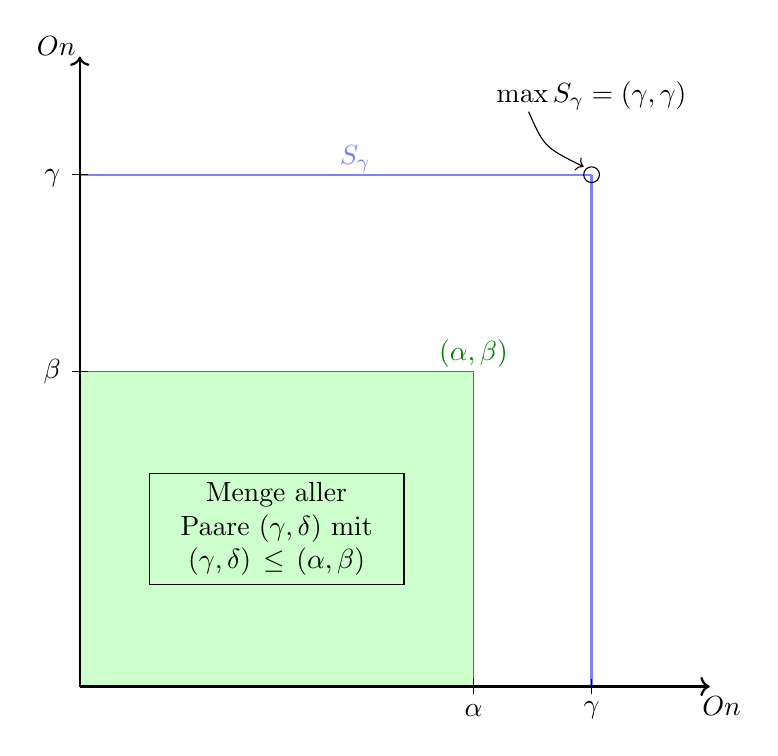
\begin{tikzpicture}
			% S_g + kleiner Zeichen + Kreis + max Schrift
			\draw[thick, blue!50!white] (6.5, 0) -- (6.5, 6.5);
			\draw[thick, blue!50!white] (0, 6.5) -- (6.5, 6.5);
			\draw[blue!50!white] (3.5, 6.7) node {$S_\gamma$};
			
			\draw (6.5, 6.5) circle (0.1);
			\draw (6.5, 7.5) node {$\max S_\gamma = (\gamma,\gamma)$};
			\draw[->] (5.7, 7.3) .. controls (5.9, 6.85) .. (6.4, 6.6);
			
			
			% (alpha, beta) Bereich + Text
			\filldraw[fill=green!20!white, draw=green!70!black] (0, 0) -- (0, 4) -- (5, 4) -- (5, 0) -- (0, 0);
			\draw[green!50!black] (5, 4.23) node {$(\alpha, \beta)$};
			\node[draw, align=center, text width=3cm] at (2.5, 2) {Menge aller Paare $(\gamma,\delta)$ mit $(\gamma,\delta)\leq(\alpha,\beta)$};
			
			% Koordinatensystem
			\draw[->, thick] (0, 0) -- (8, 0); \draw (8.15, -0.25) node {$On$};
			\draw[->, thick] (0, 0) -- (0, 8); \draw (-0.3, 8.13) node {$On$};
			
			
			% gammas auf Koordinatenachsen
			\draw[thin] (6.5, -0.1) -- (6.5, 0.1); \draw (6.5, -0.3) node {$\gamma$};
			\draw[thin] (-0.1, 6.5) -- (0.1, 6.5); \draw (-0.35, 6.45) node {$\gamma$};
			
			% alpha / beta auf Koordinatenachsen
			\draw[thin] (5, -0.1) -- (5, 0.1); \draw (5, -0.3) node {$\alpha$};
			\draw[thin] (-0.1, 4) -- (0.1, 4); \draw (-0.35, 4) node {$\beta$};	
		\end{tikzpicture}
	\end{center}
	\caption{Die grafische Darstellung von $<^\ast$.}
	\label{WohlordnungAufOrdinalHoch2}
\end{figure}

\begin{lemma}
	$<^\ast$ ist eine Wohlordnung.
\end{lemma}
\begin{proof}
	Sei $A\subseteq On\times On$ nicht-leer. Setze $\delta\coloneqq\{\delta'\in On : A\cap S_\delta'\neq\emptyset\}$. Nun ist das Minimum von $A$ das Paar $(\alpha_0,\beta_0)$ mit $\alpha_0\coloneqq\min\{\alpha\in On : \exists\beta[(\alpha,\beta)\in A\cap S_\delta]\}$ und $\beta_0\coloneqq\min\{\beta\in On : (\alpha_0,\beta)\in A\cap S_\delta\}$.
\end{proof}

\begin{definition}
	Die Gödelsche Paarfunktion $G:On\times On\to On$ ist definiert als $G(\alpha,\beta)=otp(\{(\alpha',\beta') : (\alpha',\beta')<^\ast(\alpha,\beta)\}, <^\ast)$. 
	
	Hierbei bezeichnet $otp(A, <)$ die Ordinalzahl $\alpha$ so, dass $(A,<)\cong(\alpha,<)$. Also ist $(\alpha,\beta)\downarrow^{<^\ast}\cong(G(\alpha,\beta), <)$.
\end{definition}

\begin{lemma}
	Es gilt $G(\alpha,\beta)=\{G(\alpha',\beta'):(\alpha',\beta')<^\ast(\alpha,\beta)\}$.
\end{lemma}
Der Beweis zum obigen Lemma lässt sich durch eine Graphik, welche den Isomorphismus von $((\alpha,\beta),<)$ nach $(G(\alpha,\beta), <)$ verdeutlicht.

Damit folgt dann, dass $G$ ordnungserhaltend und injektiv.

\begin{lemma}
	\begin{itemize}
		\item[a)] $G(\alpha, \beta)\geq\max\{\alpha,\beta\}$.
		\item[b)] $G[\alpha\times\alpha]=G(0,\alpha)$. Insbesondere ist $\alpha \leq G[\alpha\times\alpha]$.
		\item[c)] $G[\omega\times\omega]=\omega$.
	\end{itemize}
\end{lemma}
\begin{proof}
	a): $G(\alpha,\beta)=(\{(\alpha',\beta')\in On : (\alpha',\beta')<^\ast(\alpha,\beta)\}, <^\ast)\supset(\{(\gamma,0):\gamma<\alpha\}, <^\ast)\cong(\alpha,<)$. Es folgt, dass $G(\alpha,\beta)\geq\beta$. Analog lässt sich dies für $G(\alpha,\beta)\supseteq\beta$ zeigen.
	
	b): $\alpha\times\alpha=\{(\beta,\gamma)\in On^2 : (\beta,\gamma)<^\ast(0,\alpha)\}$. Nach dem Lemma folgt $G[\alpha\times\alpha]=G(0,\alpha)$ und wegen a) ist $\alpha\leq G(0,\alpha)=G[\alpha\times \alpha]$.
	
	c): Jedes $(m,n)\in\omega\times\omega$ hat nur endlich viele $<^\ast$-Vorgänger, also folgt $G(m,n)<\omega$. Demnach ist $G[\omega\times\omega]\leq\omega$. $G[\omega\times\omega]\geq\omega$ folgt aus b). Also muss $G[\omega\times\omega]=\omega$ gelten. Die Abbildung $G\upharpoonright\omega\times\omega$ ist also eine Bijektion von $\omega\times\omega$ nach $\omega$.
\end{proof}

Nachdem nun einige Hilfsaussagen gezeigt und diskutiert wurden können wir jetzt den Satz von Hessenberg beweisen. Zu Erinnerung: Wir müssen zeigen, dass, basierend auf ZFC, für alle Ordinale $\alpha\geq\omega$ gilt, dass $\alpha\times\alpha\sim\alpha$.
\begin{proof}[Beweis: Satz von Hessenberg]
	Wir wollen dies durch eine transfinite Induktion über $\alpha$ zeigen.
	Induktionsanfang: $\alpha=\omega$: Dies folgt aus dem Teil c) des eben bewiesenen Lemmas.
	
	Für $\alpha>\omega$ lassen sich zwei Fälle aufstellen.
	\begin{itemize}
		\item Falls ein $\beta<\alpha$ existiert mit $\beta\sim\alpha$, dann ist $\alpha\times\alpha\sim\beta\times\beta \stackrel{\text{IV}}{\sim} \beta \sim \alpha$.
		\item Sonst ist $\alpha$ ein Limesordinal, da $\beta+1\sim\beta$ wäre. Mit b) des Lemmas folgt $G[\alpha\times\alpha]\geq\alpha$. Für einen Widerspruch nehmen wir $G[\alpha\times\alpha]>\alpha$ an.
		
		Wähle $(\beta,\gamma)\in\alpha\times\alpha$ mit $G(\beta,\gamma)=\alpha$. Setze $\delta\coloneqq\{\beta,\gamma\}+1$. Also ist $(\beta,\gamma)\in\delta\times\delta$ und $\alpha=G(\beta,\gamma)\in G[\delta\times\delta]$ und daher $\alpha\subseteq G[\delta\times\delta]$.
		
		Nun ist $\alpha\stackrel{(1)}{>}\delta\stackrel{(2)}{>}\omega$, weil (1) $\alpha$ ein Limesordinal ist und (2), weil $\alpha\notin G[\omega\times\omega]$.
		
		Nach der Induktionsvoraussetzung existieren die Bijektion $g:\delta\to\delta\times\delta$ und die Abbildung $h\coloneqq G\circ g : \delta\to G[\delta\times\delta]\supseteq\alpha$.
		
		Die Umkehrabbildung $h^{-1}\upharpoonright\alpha\to\delta$ ist nun aber eine injektive Abbildung von $\alpha$ in eine Teilmenge von $\delta$. Es folgt $\alpha\sim\delta$, also müsste für $\alpha$ eigentlich der erste Fall gelten. Widerspruch!
	\end{itemize}
	
	Es gilt also $G[\alpha\times\alpha]=\alpha$ und damit ist $G\upharpoonright\alpha\times\alpha$ eine Bijektion von $\alpha\times\alpha$ nach $\alpha$.
\end{proof}

Es wurde nun also gezeigt, dass aus dem Wohlordnungssatz, daher auch dem Auswahlaxiom, die eben bewiesene Eigenschaft folgt. Die Umkehrung lässt sich aber auch zeigen.

\begin{satz}[Tarski, 1924]
	In ZF gilt: Die Aussage, dass $a\times a\sim a$ für alle unendlichen Mengen $a$ gilt impliziert das Auswahlaxiom
\end{satz}
\begin{proof}
	Sei $a$ eine Menge und $\beta\in On$ so, dass keine Surjektion von $a$ nach $\beta$ existiert. Nach Voraussetzung gilt $f:a\cup \beta \to (a\cup \beta)\times(a\cup\beta)$. Nun konstruieren wir eine Wohlordnung auf $a$.
	
	Beobachtung: $\beta\times\{x\}\not\subseteq f[a]$, denn sonst ist $h:a\to \beta\times\{x\}\to \beta$ surjektiv. Widerspruch!
	
	Also $S_b\coloneqq\{\gamma\in\beta : f(\gamma)\in\beta\times\{b\}\}\neq\emptyset$.
	
	Damit ist die Funktion $g:a\to\beta, x\mapsto \min S_x$. Dies  ist injektiv und wohldefiniert, denn $S_c\cap S_d=\emptyset$ für $c\neq d\in a$ und $g$ induziert eine Wohlordnung auf $a$ durch:
	$$b<c\text{ gdw. } g(n)<g(c).$$

	Damit wurde eine Wohlordnung gefunden und der Satz von Tarski ist bewiesen.
\end{proof}

Aus dem Satz von Hessenberg lassen sich einige Eigenschaften folgern.

Für $\kappa\in Cn$ und $\kappa\leq\lambda\in Cn^\infty$ gilt $\kappa+\lambda=\kappa\cdot\lambda=\lambda$. 
Dies lässt sich daran sehen, dass $\lambda \leq \kappa+\lambda\leq\lambda+\lambda \leq 2\cdot\lambda =\lambda$ bzw. $\lambda \leq \kappa\cdot\lambda \leq \lambda\cdot\lambda = \lambda$.

Weiter gilt für $n\geq 1$ und $\lambda \in Cn^\infty$, dass $\lambda^n=\lambda$.

\begin{satz}
	\begin{itemize}
		\item[a)] $\vert \Pot{x} \vert = 2^{\vert x \vert}$.
		\item[b)] Wenn $2\leq \kappa \leq \lambda$ mit $\kappa\in Cn, \lambda\in Cn^\infty$, dann ist $\kappa^\lambda=2^\lambda$.
	\end{itemize}
\end{satz}
\begin{proof}
		a): $\Pot{x}\sim\{f:x\to2\}$ und nach Definition ist $\vert\{f:x\to 2\}\vert=2^{\vert x \vert}$.
		
		b): $2^\lambda \leq \kappa^\lambda \leq 2^{\lambda\cdot\lambda}=2^\lambda$.
\end{proof}

Durch weitere Überlegungen kann man feststellen, dass $\vert \mathbb{Q} \vert=\vert \omega\times\omega \vert = \omega$ und $\vert \mathbb{R} \vert = \omega^\omega = 2^\omega=\vert \Pot{\mathbb{N}}\vert$. Und mit Hilfe von Satz \ref{SatzVonCantor} folgt, dass $\vert \mathbb{R} \vert \neq \vert \mathbb{Q} \vert$.

\subsubsection{Die Kontinuumshypothese (CH)}

Die Kontinuumshypothese (englisch: continuum hypothesis) besagt, dass $\omega^+=2^\omega$ oder anders ausgedrückt: $\aleph_1=2^{\aleph_0}$. Zusätzlich gibt es auch die verallgemeinerte Kontinuumshypothese (GCH), nach welche $\aleph_{\alpha+1}=2^{\aleph_\alpha}$ für alle $\alpha\in On$ gilt.
\par

Es lässt sich aber zeigen, dass \textit{CH unabhängig von ZFC ist}. Das heißt, es gilt sowohl $ZFC \not\models CH$, als auch $ZFC \not\models \neg CH$, wobei davon ausgegangen wird, dass ZFC konsistent ist und es somit überhaupt ein Modell von ZFC gibt.

Der Beweis dafür wurde von zwei Mathematikern geführt. Der erste Teil wurde von Kurt Gödel im Jahre 1938 bewiesen. Dafür hat er aus dem bekannten Stufenmodell $(S_\alpha)_{\alpha\in On}$ eine konstruierbare Hierarchie $(L_\alpha)_{\alpha\in On}$ erzeugt. Für diese gilt $L_0\coloneqq\emptyset$, für Limesordinale $\lambda$ ist $L_\lambda\coloneqq \bigcup_{\beta<\lambda}L_\beta$ und für $\alpha+1$ ist $L_{\alpha+1}\coloneqq\{x\subseteq L_\alpha : \exists a_1,\dots,a_n\exists\varphi(z,y_1,\dots,y_n) : x=\{z\in L_\alpha : (L_\alpha,\in) \models \varphi(z,a_1,\dots, a_n)\}\}$ die Menge aller Teilmengen, die sich mithilfe einer FO-Formel darstellen lassen.

Damit konnte Gödel folgern, dass $(L,\in)\models ZF$, $(L,\in)\models AC$ und $(L,\in)\models GCH$.
\\
Den zweiten Teil konnte Paul Cohen im Jahre 1963 beweisen. Sein Endresultat war, dass $ZF\notin AC$ und $ZFC \notin CH$.
\\

Daraus folgt also, dass mithilfe von ZFC nichts über die Korrektheit der Kontinuumshypothese aussagen lässt. ZFC ist also nicht vollständig. Zusätzlich nehmen die obigen Überlegungen die Konsistenz von ZFC an.

Trotz dieser Probleme mit ZFC wird dieses als \glqq Standard \grqq{} Axiomensystem angenommen. Wie im nächsten Kapitel nämlich gezeigt werden wird gilt für alle Axiomensysteme, welche genügend Aussagekraft haben, dass deren Konsistenz nicht gezeigt werden kann und sie nicht vollständig sein können.


\clearpage

\section{Die Gödelschen Unvollständigkeitssätze}

In diesem Kapitel sollen die Gödelschen Unvollständigkeitssätze behandelt werden. 
Durch diese wird einsehbar sein, dass die Unvollständigkeit von $\ZFC$, wie sie im Kapitel zur Kontinuumshypothese festgestellt wurde, nicht behoben werden kann, egal wie das Axiomensystem der Mengenlehre gewählt wird.

\subsection{Das Hilbertsche Programm}

Unter dem Hilbertschen Programm versteht man die Bestrebungen des deutschen Mathematikers David Hilbert (1862 – 1943) zur Axiomatisierung der verschiedenen Zweige der Mathematik in der Prädikatenlogik erster Ordnung.
Insbesondere sollte es möglich sein, mathematische Folgerungen auf syntaktische Ableitungen in einem formalen Kalkül zu reduzieren. Ebenso war das Ziel effektive Verfahren (heute auch Algorithmen genannt) zu konstruieren, um die Gültigkeit mathematischer Aussagen in einer Theorie zu entscheiden.
Diese Teilergebnisse sollten dann im Beweis der Widerspruchsfreiheit der Mathematik gipfeln. All diese Vorhaben kommen einem mit dem heutigen Wissen sehr utopisch vor und so soll im weiteren Verlauf des Kapitels auch bewiesen werden, dass viele Teile des Programms nicht so aufgehen, wie es sich Hilbert gewünscht hätte.\\
Dennoch konnte einige Erfolge erzielt werden:
\begin{itemize}
	\item Die Axiomatisierung wichtiger Teile der Mathematik durch geeignete Axiomensysteme konnte gezeigt werden
	\item Die Peano-Arithmetik stellt eine mögliche Axiomatisierung der bekannten Arithmetik in den natürlichen Zahlen dar
	\item Das Axiomensystem $\ZFC$ erlaubt eine Formalisierung der Mathematik innerhalb der Mengenlehre
	\item Der Begriff \textit{Beweis} konnte durch formale Systeme wie das Hilbert-Frege-System, den Sequenzenkalkül und weiteren, präzisiert werden.
	\item Durch den Beweis des Vollständigkeitssatzes von Kurt Gödel in 1931, welcher aussagt, dass $\Phi \models \psi$ äquivalent ist zu $\Phi \vdash \psi$ (für $\Phi\subseteq \FO, \psi\in \FO$), konnte gezeigt werden, dass die gewünschte Reduktion von mathematischen auf syntaktische Folgerungen gültig ist.
	\item Zuletzt konnten algorithmische Verfahren gefunden werden, um die Erfüllbarkeit bzw. Gültigkeit von \textit{Fragmenten} von $\FO$ zu entscheiden.
\end{itemize}
Jedoch haben fundamentale Resultate aus den 30er-Jahren das Hilbertsche Programm scheitern lassen:

\paragraph*{1. Gödelscher Unvollständigkeitssatz}
Jede hinreichend reichhaltige, rekursiv axiomatisierbare Theorie ist unvollständig (bspw. bezieht sich dies auf $\PA$ und $\ZFC$).

\paragraph*{Satz von Church/Turing}
Die Erfüllbarkeit bzw. Gültigkeit von $\FO$ ist unentscheidbar.

\paragraph*{2. Gödelscher Unvollständigkeitssatz}
Ist $\Phi$ ein entscheidbares, hinreichend starkes Axiomensystem, dann ist aus $\Phi$ die Widerspruchsfreiheit von $\Phi$ nicht beweisbar. Insbesondere gilt dies für $\Phi=\ZFC$.

\subsection{Theorien}

\begin{definition}[Theorie]
	Eine \textit{Theorie} $T\subseteq \FO(\tau)$ ist eine erfüllbare Satzmenge, welche unter $\models$ abgeschlossen ist. Das heißt, wenn $T\models \psi$, dann ist bereits $\psi\in T$.
\end{definition}

Im weiteren Verlauf wird die Notation $\Phi^{\models}$ für den Abschluss von $\Phi$ unter $\models$ verwendet. 
Aus dem Vollständigkeitssatz und der Definition der Theorie ergibt sich für eine Theorie $T=T^{\models}=T^\vdash$.

\begin{definition}[Vollständigkeit]
	Eine Theorie $T$ ist \textit{vollständig}, wenn für jeden Satz $\psi\in \FO(\tau)$ gilt: $\psi\in T$ oder $\neg\psi\in T$.
\end{definition}

\begin{definition}[Rekursive Axiomatisierbarkeit]
	Eine Theorie $T$ ist \textit{rekursiv axiomatisierbar}, wenn eine entscheidbare Menge 
	$\Phi\subseteq \FO$ existiert 
	mit $\Phi^{\models}=T$.
\end{definition}

\begin{satz}
	Sei $T$ eine vollständige Theorie. Dann sind äquivalent:
	\begin{enumerate}
		\item $T$ ist rekursiv axiomatisierbar.
		\item Es gibt ein rekursiv aufzählbares Axiomensystem $\Phi$ mit $T=\Phi^{\models}$.
		\item $T$ ist rekursiv aufzählbar.
		\item $T$ ist entscheidbar.
	\end{enumerate}
\end{satz}
Bemerkung: Um \textit{Rekursive Aufzählbarkeit} abzukürzen wird r.e. geschrieben, was für \textit{recursively enumerable} steht.
\begin{proof}
	\textit{1. $\Rightarrow$ 2.} Da 1. eine schwächere Aussage als 2. ist, welches 1. sogar impliziert, ist die Folgerung trivial.
	
	\textit{2. $\Rightarrow$ 3.} Wenn $\Phi$ r.e. ist, dann ist dies auch die Menge aller endlichen $\Phi_0\subseteq \Phi$. Sei $M$ nun ein Algorithmus mit Haltemenge $L(M)=\Phi$. Um zu überprüfen, ob ein $\Phi_0=\{\varphi_1,\dots,\varphi_m\}\subseteq \Phi$ ist, soll $M$ nacheinander auf $\varphi_1,\dots,\varphi_m$ angewendet werden und halten, wenn $M$ auf allen $\varphi_i$ hält.
	
	Indem man nun systematisch alle endlichen $\Phi_0\subseteq\Phi$ und alle im Sequenzenkalkül ableitbaren Sequenzen $\Phi\Rightarrow\psi$ aufzählt, erhält man ein Aufzählungsverfahren für $T$.
	
	\textit{3. $\Rightarrow$ 4.} $T$ ist vollständig, also gilt $\psi \notin T$ genau dann, wenn $\neg\psi\in T$. Mit $T$ ist also auch das Komplement von $T$ in $\FO(\tau)$ r.e. Also ist $T$ entscheidbar.
	
	\textit{4. $\Rightarrow$ 1.} Wähle $\Phi=T$. Mit der Definition ergibt sich, dass $T$ dann rekursiv aufzählbar ist.
\end{proof}

Wir betrachten nun die Struktur $\mathfrak{N}=(\mathbb{N},+,\cdot,0,1)$. Die Theorie $\TA\coloneqq \Th(\mathfrak{N})=\{\psi : \mathfrak{N}\models\psi\}$ wird als echte Arithmetik (engl.: \textit{true arithmetic}) bezeichnet. Offensichtlich ist $\TA$ vollständig.
\\
Das Axiomensystem der Peano-Arithmetik $\Phi_{\PA}$ besteht aus folgenden Axiomen:
\begin{itemize}
	\item $\forall x \neg(x+1=0)$
	\item $\forall x \forall y (x+1=y+1\rightarrow x=y)$
	\item $\forall x (x+0=x)$
	\item $\forall x \forall y(x+(y+1)=(x+y)+1)$
	\item $\forall x (x\cdot 0=0)$
	\item $\forall x \forall y (x\cdot(y+1) = (x\cdot y)+x)$
\end{itemize}
und dem Axiomenschema der vollständigen Induktion: 
$$ \forall \overline{y} ( (\varphi(0,\overline{y}) \land   \forall x 
(\varphi(x,\overline{y})\rightarrow\varphi(x+1,\overline{y}))   ) 
\rightarrow \forall x \varphi(x,\overline{y})) $$
für jede Formel $\varphi(x,\overline{y})\in \FO(\tau_{\ar})$.

Erlaubt man anstatt der Prädikatenlogik erster Ordnung auch die monadische Logik zweiter Stufe, lässt sich das Axiomenschema der vollständigen Induktion auch als allgemeines Induktionsaxiom formulieren:
$$ \forall X  (\;(X(0) \land \forall x\,(X(x)\rightarrow X(x+1)) ) 
\rightarrow \forall x\; X(x))\in MSO$$

In $\Phi_{\PA}$ wird das Induktionsaxiom dagegen aber nur für definierbare Teilmengen gefordert. Die Peano Arithmetik $\PA\coloneqq \Phi_{\PA}^{\models}$ ist rekursiv axiomatisiert und daher r.e.

\begin{definition}[Repräsentative Axiomensysteme]
	Ein Axiomensystem $\Phi$ ist \textit{repräsentativ} (oder \textit{erlaubt Kodierungen}), wenn man zu jeder Zahl $n\in \mathbb{N}$ einen Term $t_n$ angeben kann (z.B. $t_n\coloneqq\underbrace{1+\dots+1}_{n\text{-mal}}$) so, dass gilt:
	\begin{enumerate}
		\item $\Phi\vdash \neg t_n=t_m$ (für $n\neq m$)
		\item Für jede totale berechenbare Funktion $f:\mathbb{N}^k\to\mathbb{N}$ existiert eine Formel $\varphi_f(\overline{x}, y)$ so, dass für alle $n_1,\dots,n_k$
		\begin{itemize}
			\item $\Phi\vdash \exists!y \varphi_f(t_{n_1},\dots,t_{n_k}, y)$
			\item Wenn $f(n1,\dots,n_k)=m$, dann $\Phi\vdash\varphi_f(t_{n_1},\dots,t_{n_k},t_m)$
			\item Wenn $f(n_1,\dots,n_k)\neq m$, dann $\Phi\vdash\neg\varphi_f(n_1,\dots,n_k,m)$
		\end{itemize}
	\end{enumerate}	
\end{definition}

Wenn $\Phi$ repräsentativ ist, dann wird auch jede entscheidbare Relation $R\subseteq\mathbb{N}^k$ durch eine Formel $\varphi_R(x_1,\dots,x_k)$ dargestellt:
\begin{itemize}
	\item $(n_1,\dots,n_k)\in R \Rightarrow \Phi\vdash\varphi_R(t_{n_1},\dots,t_{n_k})$
	\item $(n_1,\dots,n_k)\notin R \Rightarrow \Phi\vdash\neg\varphi_R(t_{n_1},\dots,t_{n_k}$
\end{itemize}

Insgesamt lässt sich feststellen, dass $\TA, \PA$ und auch $\ZFC$ repräsentativ sind.

\begin{definition}
	Wir definieren die Funktion $[\cdot,\cdot]:\mathbb{N}\times\mathbb{N}\to\mathbb{N}, (x,y)\mapsto\frac{1}{2}(x+y)(x+y+1)+x$.
\end{definition}
\begin{lemma}
	Die Funktion $[\cdot,\cdot]$ ist bijektiv.
\end{lemma}
\begin{proof}
	Das Paar $(x,y)$ erhält die Nummer $$\left(\sum_{0\leq n < x+y}n+1\right)+x=\left(\sum_{1\leq n \leq x+y}n\right)+x=\frac{1}{2}(x+y)(x+y+1)+x=[x,y].$$
\end{proof}

Weiter lässt sich dann festlegen, dass Tupel als $[a_1,\dots,a_n]\coloneqq[a_0,[a_1,\dots,a_n]]$ definiert sind, für $n>1$. Demnach lässt sich eine definierbare Bijektion $\mathbb{N}^k\to \mathbb{N}$ für ein festes, aber beliebiges $k$ finden.

\begin{satz}[Chinesischer Restsatz]
	Seien $q_0,\dots,q_{n-1}$ paarweise teilerfremd und $q\coloneqq\prod_{i<n} q_i$. Dann ist die Funktion $$F:\mathbb{Z}/ q\mathbb{Z} \to \mathbb{Z}/q_0\mathbb{Z} \times \dots \times \mathbb{Z}/q_{n-1}\mathbb{Z}, a\mapsto(a_0,\dots,a_{n-1})$$ eine Bijektion.
\end{satz}
\begin{proof}
	Seien $a,a'\in \mathbb{Z}/q\mathbb{Z}$ so, dass $a\equiv_{q_j} a'$ für alle $j<n$. Also wird $a-a'$ von allen $q_j$ geteilt und daher, da die $q_j$ teilerfremd sind, auch von dem Produkt $q$, also ist $a\equiv_q a'$.
\end{proof}

\begin{lemma}[Gödelsches $\beta$-Lemma]
	Es gibt eine totale berechenbare Funktion $\beta:\mathbb{N}^3\to \mathbb{N}$ so, dass zu jeder endlichen Folge $(a_0,\dots,a_{n-1})$ über $\mathbb{N}$ zwei Zahlen $a,b\in\mathbb{N}$ existieren, mit $\beta(a,b,j)=a_j$ für alle $j<n$.
\end{lemma}
\begin{proof}
	Setze $\beta(x,y,z)\coloneqq x \mod (1+y(z+1))$. $\beta$ ist definierbar durch die Formel $$\varphi_\beta(x,y,z,v)\coloneqq v <1+y(z+1) \land \exists u (x=u+uy(z+1)+v).$$
	Es ist nun zu zeigen, dass sich für alle $a_0,\dots,a_{n-1}$ zwei $a,b$ angeben lassen so, dass $a\equiv a_j\mod (1+b(j+1))$ und $b\coloneqq m!$ für $m=\max\{n,a_0,\dots,a_n-1\}$.
	\\
	Behauptung: Für $0\leq i < j \leq n$ sind $1+(i+1)+b$ und $1+(j+1)+b$ teilerfremd.
	
	Andernfalls ex. ein $p>1$ mit $p \vert 1+(i+1)+b$ und $p\vert 1+(j+1)+b$.
	Es folgt, dass $p\vert (i-j)b$, aber $p\nmid b$ (sonst $p\nmid 1+(i+1)+b$), also $p\vert(i-j)$ und daher $p<n$. Dies ist aber unmöglich, da $b$ von jeder Zahl, welche kleiner als $n$ geteilt wird.
	\\ \\
	Nach dem chinesischen Restsatz existiert dann ein $a<\prod^{n-1}_{j=0}(1+b(j+1))$ mit $a\equiv a_j\mod (1+b(j+1))$ für alle $j<n$.
\end{proof}

Eine Folge $(a_0,\dots,a_{n-1})$ über $\mathbb{N}$ kodieren wir nun durch $\langle a_0,\dots,a_{n-1}\rangle\coloneqq[a,b,n]$ so, dass $\beta(a,b,i)=a_i$ für alle $i<n$, mit $b=(\max\{n,a_0,\dots,a_{n-1}\})!$. Weiter ist die Länge solch einer Folge $\ln(\langle a_0,\dots, a_{n-1}\rangle)\coloneqq n$ und $\pi_i(\langle a_0,\dots, a_{n-1})=a_i$.

Es lässt sich feststellen, dass $[\cdot,\cdot]$, $\beta$, $\ln$ und $\pi$ in $\TA$, $\PA$ und $\ZFC$ definierbar sind.


\subsection{Kodierung von Turing Maschinen}

Mit den Ergebnissen aus dem vorherigen Kapitel ist es nicht schwer Turing Maschinen zu kodieren und mithilfe dieser gewisse Widersprüche zu zeigen.

Eine Turing Maschine (kurz: TM) ist ein Tupel $M=(Q,\Sigma, \delta, q_0, F)$ und eine Konfiguration einer TM ist ein Tripel $c=[q,w,p]$, wobei $q<\vert Q\vert$, $w=(w_0,\dots,w_{n-1})\in \Sigma^\ast \text{ mit } w_i\leq \vert \Sigma\vert$, und $p\leq \vert w \vert$. Es soll zudem noch bemerkt werden, dass die Relation $\vdash_M$ die Nachfolgerrelation ist. $x\vdash_M y$ gilt also genau dann, wenn $y$ in $M$ eine gültige Nachfolgerkonfiguration ist.

Sei nun $\Phi\in\{\TA,\Phi_{\PA},\ZFC\}$ und $M$ eine TM. Es gibt Formeln $\Konf_M(x)$, $\Start_m(x,y)$, $\End_M(x,y)$ und $\Lauf_M(x)$ mit 
\begin{itemize}
	\item $\Phi\vdash \Konf_M(n)$ gdw. $n$ kodiert eine gültige Konfiguration von $M$, also $n=[q,w,p]$.
	\item $\Phi\vdash \Start_M(n,m)$ gdw. $n$ kodiert die Inputkonfiguration von $M$ auf $m$.
	\item $\Phi\vdash \End_M(n,m)$ gdw. $n$ kodiert eine Endkonfiguration von $M$ mit Bandinschrift (Output) $m$.
	\item $\Phi\vdash \Lauf_M(x)$ gdw. $x$ beschreibt eine gültige Berechnung von $M$, d.h. eine Folge $x=\langle c_0,\dots,c_n\rangle$ mit $\Konf_M(c_i)$ und $c_i\vdash_M c_{i+1}$.
\end{itemize}

Mit diesen Formeln und des Erlaubens von Kodierungen von $\TA$, $\Phi_{\PA}$ und $\ZFC$ erhält man die Folgerung, welche zuerst von Tarski formuliert wurde:
$$\boxed{\TA \text{ ist unentscheidbar}}$$
Der Beweis lässt sich mithilfe des Halteproblems führen. Angenommen, $\TA$ wäre entscheidbar. Da $\TA$ vollständig ist, ließe sich mithilfe der obigen Formeln für beliebige TMs entscheiden, ob gegebene Läufe gültig sind. Mithilfe der Formeln würde man dann das Halteproblem lösen können. Nach Turing (1937) ist dies aber nicht möglich, weshalb $\TA$ nicht entscheidbar sein kann.

Die exakt gleiche Argumentation lässt sich auch auf $\PA$ und $\ZFC^{\models}$ übertragen, weshalb diese ebenfalls nicht entscheidbar sein können.

Dies führt zum ersten Unvollständigkeitssatz von Gödel:

\begin{satz}[1. Gödelscher Unvollständigkeitssatz]
	\begin{enumerate}
		\item Es gibt kein entscheidbares Axiomensystem für $\TA$.
		\item $\PA$ ist unvollständig
	\end{enumerate}
	\label{unvollst1}
\end{satz}
\begin{proof}
\textit{1.} ist zwar die gleiche Aussage wie die Folgerung Tarskis, Gödel hat dies aber über einen anderen Weg noch vor Turings Entdeckung der Unentscheidbarkeit des Halteproblems gezeigt, welchen wir und im Folgenden anschauen möchten.

\textit{2.} ist durch einen Widerspruch mithilfe des ersten Teiles möglich. Wäre $\PA$ vollständig, dann wäre es ein Axiomensystem für $\TA$. Nach \textit{1.} wäre $\PA$ dann aber nicht entscheidbar, war entgegen der Definition von $\PA$ geht. Also muss $\PA$ unvollständig sein.
\end{proof}


\subsection{Gödelisierung von Termen und Formeln}

Wie im vorherigen Kapitel erwähnt hat Gödel einen anderen Weg für seine Unvollständigkeitssätze verwendet, unter anderem, weil Turing seinen Beweis erst einige Jahre nach Gödel veröffentlicht hat. In diesem Kapitel soll nun der Beweisweg von Gödel betrachtet werden.
\\
Als Gödelisierung wird das Verfahren bezeichnet, den Termen und Formeln einer Logik eine eindeutige, natürliche Zahl zuzuordnen. Ein Term $t$ wird zu einer natürlichen Zahl $\opencorner t\closecorner\in \mathbb{N}$ und eine Formel $\phi$ wird zu der Zahl $\opencorner\varphi\closecorner\in \mathbb{N}$. Für eine Formel $\theta(x)$ und $k\in \mathbb{N}$ schreibt man $\theta(k)$ für $\theta[x/\underbrace{1+\dots+1}_{k\text{-mal}}]$, also das Ersetzen von jedem Vorkommen von $x$ in $\theta$ durch einen Term, welcher zu $k$ auswertet.

\begin{satz}[Fixpunktsatz]
	$\Phi$ erlaube Kodierungen. Zu jeder Formel $\psi(x)\in \FO({+,\cdot,0,1})$ ex. ein Satz $\varphi$ mit $\Phi\vdash\varphi\leftrightarrow\psi(\opencorner \varphi \closecorner)$.
\end{satz}

Der Fixpunktsatz lässt sich auch anders formulieren: Aus jeder Formel $\psi(x)\in \FO({+,\cdot,0,1})$ wird eine Funktion $f_\psi, \varphi\mapsto\psi(\opencorner\varphi\closecorner)$ gebildet. Jede solche Funktion hat einen bis auf Äquivalenz bestimmten Fixpunkt.

\begin{proof}
	Sei $f:\mathbb{N}\times\mathbb{N}\to \mathbb{N}$ die Funktion mit $f(\opencorner\theta(x)\closecorner, k)\coloneqq\opencorner\theta(k)\closecorner$ und $f(n,k)=0$, wenn $n$ nicht die Gödelnummer einer Formel $\theta(x)$ ist.
	
	Da $f$ berechenbar ist, gibt es eine Formel $\alpha(x,y,z)$ mit $\Phi\vdash\alpha(n,k,m)$ gdw. $m=f(n,k)$.
	Für eine gegebene Formel $\psi(x)$ setze $\theta(x)\coloneqq\forall z (\alpha(x,x,z)\rightarrow\psi(z))$ und $\varphi\coloneqq\theta(\opencorner\theta\closecorner)$.
	Dann gilt $f(\opencorner\theta\closecorner,\opencorner\theta\closecorner)=\opencorner\varphi\closecorner$, also 
	\[
	\Phi\vdash\alpha(\opencorner\theta\closecorner,\opencorner\theta\closecorner,\opencorner\varphi\closecorner) \tag*{$(\ast)$}
	\]
	Es bleibt zu zeigen, dass $\Phi\vdash\varphi \leftrightarrow \psi(\opencorner\varphi\closecorner)$ gilt.
	\begin{itemize}
		\item[$\Rightarrow$:] Man betrachte die Sequenz $\Phi\vdash(\varphi\land\alpha(\opencorner\theta\closecorner,\opencorner\theta\closecorner,\opencorner\varphi\closecorner))\rightarrow\psi(\opencorner\varphi\closecorner)$. 
		Zur Erinnerung ist $\varphi$ definiert als $\varphi\coloneqq\forall z (f(\opencorner\theta\closecorner,\opencorner\theta\closecorner)=z\rightarrow\psi(z))$. 
		Falls nun also $\varphi$ und $\alpha(\opencorner\theta\closecorner,\opencorner\theta\closecorner,\opencorner\varphi\closecorner)$ gilt, dann muss, wegen der Aussage von $\varphi$, auch $\psi(\opencorner\varphi\closecorner)$ gelten.
		\\
		Durch $(\ast)$ folgt dann $\Phi\vdash\varphi\rightarrow\psi(\opencorner\varphi\closecorner)$
		
		\item[$\Leftarrow$:] Es gilt $\Phi\vdash \exists!z \alpha(\opencorner\theta\closecorner, \opencorner\theta\closecorner, z)$. Die Existenz folgt aus $(\ast)$ und die Eindeutigkeit, da $\alpha$ eine Funktion repräsentiert. Demnach ist dann
		\[\Phi\vdash\forall z (\alpha(\opencorner\theta\closecorner, \opencorner\theta\closecorner, z)\rightarrow z=\opencorner\varphi\closecorner).\] Mit der Definition von $\varphi$ folgt dann \[\Phi\vdash\psi(\opencorner\varphi\closecorner)\rightarrow\underbrace{(\forall z (f(\opencorner\theta\closecorner,\opencorner\theta\closecorner)=z\rightarrow\psi(z)))}_\varphi\] bzw. $\Phi\vdash\psi(\opencorner\varphi\closecorner)\rightarrow\varphi$.
	\end{itemize}
\end{proof}

\begin{satz}
	Sei $\mathfrak{A}$ eine Struktur deren Universum $\mathbb{N}$ umfasst so, dass $\Th(\mathfrak{A})$ Kodierungen erlaubt. Dann existiert keine Formel $\True_\mathfrak{A}(x)$ so, dass für alle $\psi$ gilt: $\mathfrak{A}\models\psi\Leftrightarrow\mathfrak{A}\models \True_\mathfrak{A}(\opencorner\psi\closecorner)$.
\end{satz}
\begin{proof}
	Wir nehmen an $\True_\mathfrak{A}(x)$ existiert.
	Nach dem Fixpunktsatz existiert zu $\neg \True_\mathfrak{A}(x)$ ein Fixpunkt $\varphi$ so, dass
	\[\Th(\mathfrak{A})\vdash\varphi\leftrightarrow\neg \True_\mathfrak{A}(\opencorner\varphi\closecorner). \tag{$\ast$}\]
	Informell \glqq behauptet\grqq{} $\varphi$, dass $\varphi$ falsch ist. Nun folgt
	\[\mathfrak{A}\models\varphi \xLeftrightarrow{(\ast)} \mathfrak{A}\models\neg \True_\mathfrak{A}(\opencorner\varphi\closecorner) \xLeftrightarrow{\text{Def. von } \True_\mathfrak{A}}\mathfrak{A}\not\models\varphi.\] Widerspruch!
\end{proof}
Die wahren Sätze von $\Th(\mathfrak{N})$ sind also nicht in $\Th(\mathfrak{N})$ repräsentierbar. Anders formuliert:

Sei $T$ eine repräsentative und vollständige Theorie. Dann ist $T$ nicht in $T$ definierbar. Das heißt es gibt keine Formel $\True_T(x)$ mit $$\psi\in T\Leftrightarrow \True_T(\opencorner\psi\closecorner)\in T.$$
Damit folgt wieder der 1. Gödelsche Unvollständigkeitssatz (die genau Definition kann in Satz \ref{unvollst1} gefunden werden): 

Sei $T$ rekursiv axiomatisierbar und repräsentativ. Dann ist $T$ unvollständig. Sonst wäre $T$ entscheidbar und da $T$ repräsentativ ist, wäre die entscheidbare Menge $\{\opencorner\psi\closecorner:\psi\in T\}$ in $T$ definierbar.
\\
\par
Sei $\Phi$ entscheidbar und repräsentativ. Nun nehmen wir uns eine geeignete Kodierung von Ableitungen im Sequenzenkalkül und betrachten $B\subseteq\mathbb{N}\times\mathbb{N}$ mit 
$$(n,m)\in B \text{ gdw. } n=\opencorner \Phi_0\Rightarrow\psi \closecorner \text{ gültige Sequenz}, \Phi_0\subseteq\Phi \text{ endlich und } m=\opencorner\psi\closecorner.$$
$B$ ist entscheidbar, also existiert eine Formel $\Beweis_\Phi(x,y)$ so, dass $\Phi\vdash \Beweis_\Phi(n,m)$ gdw. $(n,m)\in B$. 
Weiter werden die Formeln $\Abl_\Phi(x)\coloneqq\exists y \Beweis_\Phi(y,x)$ und $\Wf_\Phi\coloneqq \neg \Abl_\Phi(\opencorner\neg0=0\closecorner)$ definiert. Dabei bezeichnet $\Abl_\Phi(x)$, dass es einen Beweis für $x$ gibt und $\Wf_\Phi$ drückt die Widerspruchsfreiheit von $\Phi$ aus.

\begin{satz}[2. Gödelscher Unvollständigkeitssatz]
	Ist $\Phi\supseteq\Phi_{\PA}$ entscheidbar und konsistent, dann ist $\Phi\nvdash \Wf_\Phi$.
\end{satz}
\begin{proof}
	Nach dem Fixpunktsatz existiert ein Satz $\varphi$ mit $\Phi\vdash\varphi\leftrightarrow\neg \Abl_\Phi(\opencorner\varphi\closecorner)$. Ähnlich zum vorherigen Beweis \glqq behauptet\grqq{} $\varphi$ seine eigene Unbeweisbarkeit. Nun ist $\Phi\nvdash\varphi$, da sonst eine Ableitung $\Phi_0\Rightarrow\varphi$ mit endlichem $\Phi_0\subseteq\Phi$ existiert und somit würde $\Phi\vdash \Abl_\Phi(\opencorner\varphi\closecorner)$ folgen und damit $\Phi\vdash \neg\varphi$. Also ist $\Wf_\Phi\rightarrow\neg \Abl_\Phi(\opencorner\varphi\closecorner)$.
	
	Man kann diesen Beweis in $\Phi\supseteq\Phi_{\PA}$ nachvollziehen und zeigen, dass $\Phi\vdash \Wf_\Phi \rightarrow \neg \Abl_\Phi(\opencorner\varphi\closecorner)$. Dies ist aber sehr schwer und technisch, weshalb dies nicht hier vorgeführt werden soll.
	\\
	Wenn nun aber $\Phi\vdash \Wf_\Phi$ gelten würde, dann auch $\Phi\vdash \neg \Abl_\Phi(\opencorner\varphi\closecorner)$ und damit $\Phi\vdash \varphi$. Widerspruch!
\end{proof}
Aus einem repräsentatives Axiomensystem lässt sich damit also nicht die Widerspruchsfreiheit von diesem folgern. Damit gilt also $\ZFC\not\vdash\Wf_{\ZFC}$.





\clearpage

\section{Modelltheorie}

Nachdem in den letzten Teilen wichtige Konzepte der Mengenlehre und die Gödelschen Unvollständigkeitssätze vermittelt wurden, sollen werden hier nun zentrale Ideen der Modelltheorie gezeigt.

\subsection{Erhaltungssätze (Charakterisierungssätze)}

Ein wichtiges Ziel der Modelltheorie ist es, einen Zusammenhang zwischen Syntax und Semantik zu bilden. Allgemein lässt sich dies formalisieren: Eine Formel $\psi\in FO$ hat eine semantische Eigenschaft $P$ gdw. wenn $\psi$ äquivalent zu einer Formel in einem Fragment $F_p\subseteq FO$ ist.

Beispiele dafür sind der Satz von \textit{\L os-Tarski} und \textit{Satz von Benthem}.

\paragraph{Satz von \L o\'{s}-Tarski}
$\psi\in FO$ ist erhaltend unter Substrukturen (d.h. wenn $\mathfrak{B}\models \psi$ und $\mathfrak{A}\subseteq\mathfrak{B}$, dann ist auch $\mathfrak{A}\models\psi$) gdw. $\psi$ äquivalent ist zu einer universellen Formel $\forall \bar{x}(\varphi)$, wobei $\varphi$ quantorenfrei ist.

\paragraph{Satz von van Benthem}
$\psi(x)\in FO$ ist invariant unter Bisimulation (d.h. wenn $\K\models \psi(v)$ und $\K,v\sim \K',v'$, dann gilt auch $\K'\models \psi(v')$) gdw. $\psi(x)$ äquivalent zu einer Formel $\psi'\in ML$ ist.

In beiden Fällen gilt, dass die Richtung von Syntax zur Semantik trivial ist. Beispielsweise ist die Bisimulations-Invarianz von zu einer Modallogischen Formel äquivalenten $FO$-Formel klar. Die Rückrichtung ist aber alles andere als offensichtlich und werden daher noch genauer in diesem Kapitel betrachtet.

\subsection*{Refresher zur Modallogik}

Für eine Formel $\psi$ gilt $\psi\in ML$ (Modallogik), wenn $\psi$ induktiv definiert ist, als
\[\psi\coloneqq P_i \,\vert\, \neg\psi \,\vert\, \psi\land\psi \,\vert\, \psi\lor\psi \,\vert\, \psi\rightarrow\psi \,\vert\, \lozenge\psi \,\vert\, \square\psi.\]

Modell einer Modallogischen Formel ist eine Kripkestruktur $\K=(V,(P_i)_{i\in I}, E)$. Wobei $V$ eine Menge an Knoten, $E$ eine zweistellige Kantenrelation und $P_i$ für jedes $i\in I$ eine einstellige Relation ist, welche die Eigenschaften von Knoten darstellt.
\\
\\
Semantisch ist $ML$ definiert als
\begin{itemize}
	\item $\K,v\models P_i$ gdw. $v\in P_i$.
	\item Die Junktoren $\land,\lor,\rightarrow$ sind wie aus $AL$ oder $FO$ bekannt.
	\item $\K,v\models \lozenge \psi$ genau dann, wenn es ein $w\in vE=\{w:(v,w)\in E\}$ gibt, mit $\K,w\models \psi$.
	\item $\K,v\models \square \psi$ genau dann, wenn für alle $w\in vE$ gibt, mit $\K,w\models \psi$.
\end{itemize}
Die Modallogik lässt sich in die Prädikatenlogik einbetten. Es gibt also eine Abbildung mit $\psi\mapsto \psi^\ast(x)$, bzw. nach Formelaufbau:

\begin{itemize}
	\item $P_i\mapsto P_i x$
	\item $\psi_1\circ \psi_2\mapsto \psi_1^\ast(x)\circ\psi_2^\ast(x)$ für $\circ\in\{\land,\lor,\rightarrow\}$
	\item $\lozenge\psi\mapsto\exists y (Exy \land \psi^\ast(y))$
	\item $\square\psi \mapsto \forall y (Exy\rightarrow \psi^\ast(y))$
\end{itemize}
Das Bild dieser Abbildung wird als modales Fragment der Prädikatenlogik bezeichnet.
\\
\\
Eine Bisimulation zwischen zwei Transitionssystemen $\K=(V,(P_i)_{i\in I}, E)$ und $\K'=(V',(P_i')_{i\in I}, E')$ ist eine Relation $Z\subseteq V\times V'$ so, dass für alle $(v,v')\in Z$ gilt:
\begin{itemize}
	\item $v\in P_i\Leftrightarrow v'\in P_i'$
	\item Hin: Zu jedem Knoten $w\in vE$ existiert ein $w'\in v'E'$ so, dass $(w,w')\in Z$.
	\item Her: Zu jedem Knoten $w'\in v'E'$ existiert ein $w\in vE$ so, dass $(w,w')\in Z$,
\end{itemize}
Es lässt sich erkennen, dass $ML$ Bisimulationsinvariant ist. Das heißt, wenn $\K,v\models \psi$ und $\K,v\sim \mathfrak{K'},v'$, dann ist auch $\K',v'\models \psi$.


\subsection*{Weiter mit Erhaltungssätzen}

\begin{definition}[Existenziell-positiv]
	Eine $FO$-Formel ist \textit{existenziell positiv} ($\Sigma_1^+$-Formel), wenn sie weder Allquantoren, noch Negationen oder Implikationen enthält, also aus Atomen mit $\land$, $\lor$ und $\exists$ aufgebaut ist.
\end{definition}

\begin{definition}[Existenzielle und universelle Formeln]
	Eine $FO$-Formel ist existenziell ($\Sigma$-Formel), wenn sie die Form $\exists \bar{x} \varphi$ mit quantorenfreiem $\varphi$ hat.
	
	Eine $FO$-Formel ist universell ($\Pi_1$-Formel), wenn sie die Form $\forall \bar{x} \varphi$ mit quantorenfreiem $\varphi$ hat.
\end{definition}
Induktiv ist weiter definiert, dass eine Formel $\psi$ eine $\Sigma_{n+1}$-Formel ist, wenn $\psi=\exists\bar{x}\varphi$ gilt und $\varphi$ eine $\Pi_n$-Formel ist. Dual ist dies für $\Pi_{n+1}$-Formeln definiert. Eine $\Pi_{n+1}$-Formel ist von der Form $\forall \bar{x}\varphi$ für ein $\varphi$, welches eine $\Sigma_n$-Formel ist. Offensichtlich sind diese Formeln in Pränex-Normalform. Auch lässt sich erkennen, dass wenn $\varphi$ eine $\Sigma_n$-Formel ist, $\neg\varphi$ eine $\Pi_n$-Formel wird.

\begin{definition}[Abgeschlossenheit]
	Eine Formel $\psi(x)$ ist abgeschlossen unter einer Abbildung $f:\mathfrak{A}\to\mathfrak{B}$, wenn für alle $\bar{a}$ aus $\mathfrak{A}$ gilt $\mathfrak{A}\models\psi(\bar{x})\Rightarrow\mathfrak{B}\models\psi(f\bar{a})$.
\end{definition}

Ein \textit{Homomorphismus} $h$ ist eine Abbildung von $\mathfrak{A}$ nach $\mathfrak{B}$, für welche gilt, wenn $\bar{a}\in R^\mathfrak{A}$, dann ist $(h \bar{a})\in R^\mathfrak{B}$ für ein Relationssymbol $R$ und analog für Funktionen.

Verglichen dazu ist ein \textit{starker Homomorphismus} ein \textbf{injektiver} Homomorphismus $h$, für den gilt $\bar{a}\in R^\mathfrak{A}$ \textbf{gdw.} $(h \bar{a})\in R^\mathfrak{B}$. Einen starken Homomorphismus nennt man auch eine \textit{Einbettung}.

\begin{lemma}
	Jede $\Sigma^+_1$-Formel bleibt unter Homomorphismen erhalten.
	\label{Sigma1UnterHom}
\end{lemma}
\begin{proof}
	Sei $h:\mathfrak{A}\to\mathfrak{B}$ ein Homomorphismus. Zunächst gilt für jeden Term $t(\bar{x})$:
	\[h(\llbracket t(\bar{a})\rrbracket^\mathfrak{A})=\llbracket t(h\bar{a})\rrbracket^\mathfrak{B}, \tag{$(\ast)$}\]
	denn:
	\begin{itemize}
		\item $t\coloneqq x_i$: klar, da beide Seiten den Wert $ha_i$ \glqq erhalten\grqq{}.
		\item $t\coloneqq gt_1\dots t_k$: Dann ist
		\begin{alignat*}{2}
			h\llbracket t(\bar{a})\rrbracket^\mathfrak{A} 
			&= &&h(g^\mathfrak{A}(\llbracket t_1(\bar{a})\rrbracket^\mathfrak{A},\dots,\llbracket t_k(\bar{a})\rrbracket^\mathfrak{A})) \\
			\overset{h \text{ Hom.}}&{=} &&g^\mathfrak{B}(h\llbracket t_1(\bar{a})\rrbracket^\mathfrak{A},\dots,h\llbracket t_k(\bar{a})\rrbracket^\mathfrak{A}) \\
			\overset{\text{IV.}}&{=} &&g^\mathfrak{B}(\llbracket t_1(h\bar{a})\rrbracket^\mathfrak{B},\dots,\llbracket t_k(h\bar{a})\rrbracket^\mathfrak{B}) \\
			&= &&\llbracket t(h\bar{a})\rrbracket^\mathfrak{B}.
		\end{alignat*}
	\end{itemize}
	Durch eine Induktion über den Formelaufbau lässt sich dann diese Eigenschaft auch für Formeln $\psi$ feststellen:
	\begin{itemize}
		\item $\psi\coloneqq t_1(\bar{x})=t_2(\bar{x})$:
		\begin{alignat*}{2}
			\mathfrak{A}\models t_1(\bar{a})=t_2(\bar{a})
			&\Longleftrightarrow &&\llbracket t_1(\bar{a})\rrbracket^\mathfrak{A} = \llbracket t_2(\bar{a})\rrbracket^\mathfrak{A} \\
			&\Longrightarrow &&h\llbracket t_1(\bar{a})\rrbracket^\mathfrak{A} = h\llbracket t_2(\bar{a})\rrbracket^\mathfrak{A} \tag{$\vartriangle$}\\
			\overset{(\ast)}&{\Longleftrightarrow} &&\llbracket t_1(h\bar{a})\rrbracket^\mathfrak{B} = \llbracket t_2(h\bar{a})\rrbracket^\mathfrak{B} \Leftrightarrow \mathfrak{B}\models t_1(h\bar{a})=t_2(h\bar{a}).
		\end{alignat*}
		
		\item $\psi\coloneqq R t_1(\bar{x}),\dots,t_k(\bar{x})$:
		\begin{alignat*}{2}
			\mathfrak{A}\models R t_1(\bar{a}),\dots,t_k(\bar{a})
			&\Longleftrightarrow &&(\llbracket t_1(\bar{a})\rrbracket^\mathfrak{A},\dots,\llbracket t_k(\bar{a})\rrbracket^\mathfrak{A})\in R^\mathfrak{A} \\
			\overset{h\text{ Hom.}}&{\Longrightarrow} &&(h\llbracket t_1(\bar{a})\rrbracket^\mathfrak{A},\dots,h\llbracket t_k(\bar{a})\rrbracket^\mathfrak{A})\in R^\mathfrak{B} \tag{$\bigcirc$} \\
			\overset{(\ast)}&{\Longleftrightarrow} &&(\llbracket t_1(h\bar{a})\rrbracket^\mathfrak{B},\dots,\llbracket t_k(h\bar{a})\rrbracket^\mathfrak{B})\in R^\mathfrak{B} \Leftrightarrow \mathfrak{B}\models R t_1(h\bar{a}),\dots,t_k(h\bar{a}).
		\end{alignat*}
		
		\item Die Fälle $\psi\coloneqq\varphi\land\varphi'$ und $\psi\coloneqq \varphi\lor \varphi'$ sind klar.
		
		\item $\psi\coloneqq \exists y \varphi(\bar{x},y)$:
		\begin{alignat*}{2}
			&  &&\mathfrak{A}\models \exists y \varphi(\bar{a},y) \\
			&\Longrightarrow &&\text{es ex. } b \text{ mit } \mathfrak{A}\models\varphi(\bar{a},b) \\
			\overset{\text{IV}}&{\Longrightarrow} &&\mathfrak{B}\models \varphi(h\bar{a},hb) \Rightarrow \mathfrak{B}\models \exists y \varphi(h\bar{a},y).
		\end{alignat*}
	\end{itemize}
\end{proof}

\begin{lemma}
	$\Sigma_1$-Formeln $\psi(\bar{x})$ bleiben unter Einbettung erhalten.
\end{lemma}
\begin{proof}
	Sei $h$ eine Einbettung. Ohne Einschränkung lässt sich voraussetzen, dass $\psi(\bar{x})$ in Negations-NF ist. Nun lässt sich die Behauptung durch eine Induktion über den Formelaufbau wie oben zeigen:
	\begin{itemize}
		\item Für $\psi\coloneqq t_1=2t_2$ oder $\psi\coloneqq R t_1,\dots,t_n$ lässt sich dies genauso wie oben zeigen.
		\item Da $h$ injektiv ist, gilt die Folgerung $(\vartriangle)$ auch in die andere Richtung. Man erhält also eine Kette an Äquivalenzen. Dadurch lässt sich diese analog auf den hier beschriebenen Fall $\psi$ anwenden.
		\item Falls $\psi\coloneqq\neg R t_1,\dots,t_n$ lässt sich das Argument wie im vorherigen Beweis verwenden. Die Folgerung von $(\bigcirc)$ wird aber eine Äquivalenz, da $h$ ein starker Homomorphismus ist.
		\item Die Fälle $\psi\coloneqq\varphi\land\varphi'$, $\psi\coloneqq\varphi\lor\varphi'$ und $\exists y \varphi(\bar{x},y)$ lassen sich genauso wie oben beweisen.
	\end{itemize}
\end{proof}

\begin{lemma}
	$\Pi_1$-Formeln bleiben unter Substrukturen erhalten.
	\label{Pi1UnterSubstruk}
\end{lemma}
\begin{proof}
	Seien $\A,\B$ zwei Strukturen mit $\A\subseteq\B$ und $\psi(\bar{x})$ eine $\Pi_1$-Formel. Angenommen, es gilt $\A\models\neg\psi(\bar{a})$ und $\B\models\psi(\bar{a})$ für $\bar{a}$ aus $A$. Dann ist $\neg\psi(\bar{x})$ aber äquivalent zu einer $\Sigma_1$-Formel. Mit Lemma \ref{Sigma1UnterHom} folgt aber $\A\models\neg\psi(\bar{x})\Rightarrow\B\models\neg\psi(\bar{a})$. Widerspruch!
\end{proof}

\begin{definition}
	Eine Folge $(\A)_{i<\alpha}$ von $\tau$-Strukturen ist eine \textit{Kette}, wenn jeweils $\A_i\subseteq\A_j$ für $i<j$. Die Vereinigung $\bigcup_{i<\alpha}\A_i$ einer solchen Kette ist die Struktur $\A$ mit Universum $A=\bigcup_{i<\alpha}A_i$ und
	\begin{itemize}
		\item $\bar{a}\in R^\A$ gdw. $\bar{a}\in R^{\A_i}$ für ein $i<\alpha$ (und daher für alle $j<\alpha$ mit $\bar{a}\in A_j$).
		\item $f^\A(\bar{a})=b$ gdw. $f^{\A_i}\bar{a}=b$ für ein (und dadurch alle) $i<\alpha$ mit $\bar{a}\in A_i$.
	\end{itemize}
\end{definition}
$\varphi(x)$ bleibt Erhalten unter Vereinigung von Ketten, wenn für jede Kette $(\A_i)_{i<\alpha}$ mit $\bar{a}\in A_0$ und $\A_i\models\varphi(\bar{a})$ für alle $i$, dann auch $\bigcup_{i<\alpha}\A_i \models \varphi(\bar{a})$ gilt.

Dies sind nicht alle Formeln. Sei bspw. $\A_i=(\{0,\dots,i\},a^{\N})$. Jedes $\A_i$ hat ein maximales Element, aber $\bigcup\A_i=(\N,<)$ nicht. Das heißt, es gibt $\Sigma_2$-Formeln, welche nicht unter Vereinigung von Ketten erhalten bleiben ($\exists x \forall y (y\leq x)$).

\begin{lemma}
	$\Pi_2$-Formeln bleiben erhalten unter Vereinigung von Ketten.
\end{lemma}
\begin{proof}
	Sei $(\A_i)_{i<\alpha}$ eine Kette, $\A\coloneqq\bigcup_{i<\alpha}\A_i$ und $\bar{a}\subseteq A_0$. Weiter sei $\forall \bar{y} \varphi(\bar{x},\bar{y})$ eine $\Pi_2$-Formel (also $\varphi(\bar{x},\bar{y})$ eine $\Sigma_1$-Formel) so, dass $\A_i\models\forall \bar{y} \varphi(\bar{a},\bar{y})$ für alle $i<\alpha$.
	
	Nun ist zu zeigen, dass $\A\models\forall \bar{y} \phi(\bar{a},\bar{y})$. Angenommen, es existiert ein $\bar{b}\subseteq\A$ mit $\A\models\neg\varphi(\bar{a},\bar{b})$. Da $\vert\bar{b}\vert$ endlich ist, existiert ein $j<\alpha$ mit $\bar{b}\subseteq A_j$. 
	Da $\neg\varphi$ äquivalent zu einer $\Pi_1$-Formel ist und $\A_j\subseteq\A$, folgt wegen Lemma \ref{Pi1UnterSubstruk}, dass $\A_i\models\neg\varphi(\bar{a},\bar{b})$ im Widerspruch zu $\A_j\models\forall\bar{y}\varphi(\bar{a},\bar{y})$.
\end{proof}

\begin{definition}
	Sei $\A$ eine $\tau$-Struktur und $B\subseteq A$. Dann ist $\A_B$ die Expansion von $\A$ um je eine Konstante für $b$ für jedes Element $b\in B$. Ist $T$ eine vollständige Theorie und $\A\models T$, dann ist $T(B)\coloneqq Th(\A_B)$. Im Fall $B=A$ nenne wir $T(A)\coloneqq Th(\A_A)$ das \textit{elementare Diagramm} von $\A$.
\end{definition}
Im Gegensatz dazu ist das Diagramm $D(\A)$ definiert durch $$D(\A)\coloneqq\{\varphi(\bar{a})\in T(A) : \varphi \text{ atomar oder negiert-atomar}\}$$.

\begin{definition}
	$\A$ ist eine \textit{elementare Substruktur} von $\B$ ($\A\preceq\B$), wenn $\A\subseteq\B$ und für jede Formel $\varphi(\bar{x})\in FO$ und alle $\bar{a}$ aus $A$ gilt: $\A\models\varphi(\bar{a})\Leftrightarrow\B\models\varphi(\bar{a})$.
\end{definition}
Dies soll durch zwei Beispiele genauer beleuchtet werden. 

\begin{itemize}
	\item $\A=(\Q,<),\B=(\R,<)$. Dann lässt sich leicht feststellen, dass $\A\preceq\B$.
	\item $\A=(\N\setminus\{0\},<), \B=(\N,<)$. Es gilt $\A\subseteq\B$ und sogar $\A\cong\B$. Aber trotzdem ist $\A\not\preceq\B$. Sei $\varphi(x)$ in einer Struktur wahr, gdw. $x$ das kleinste Element der Struktur ist. Dann ist $\A\models\varphi(1)$, aber $\B\not\models\varphi(1)$.
\end{itemize}

\begin{satz}[Tarski-Vaught-Test]
	Sei $\A\subseteq\B$. Nun sind äquivalent:
	\begin{enumerate}
		\item $\A\preceq \B$.
		\item Für jede Formel $\varphi(\bar{x},y)$ und alle $\bar{a}$ aus $\A$ gilt: $\B\models \exists y \varphi(\bar{a},y)\Rightarrow \B\models\varphi(\bar{a},a')$ für ein $a'\in A$.
	\end{enumerate}
\end{satz}
\begin{proof}
	\textit{1. $\Rightarrow$ 2.}: Sei $\A\preceq\B$ und $\B\models\exists y \varphi(\bar{a},y)$. Dann gilt $\A\models\exists y \varphi(\bar{a},y)$, das heißt $\A\models\varphi(\bar{a},a')$ für ein $a'\in A$. Da $\A\preceq\B$, folgt $\B\models\varphi(\bar{a},a')$.
	
	\textit{2. $\Rightarrow$ 1.}: Das Kriterium des Tests sei erfüllt. Nun ist zu zeigen, dass für jede Formel $\psi(\bar{x})$ und $\bar{a}$ aus $\A$ gilt: $\A\models\psi(\bar{a})\Leftrightarrow \B\models\psi(\bar{a})$. Dies soll wieder durch eine Induktion über den Formelaufbau passieren.
	
	\begin{itemize}
		\item Die atomaren Fälle $\psi\coloneqq x=y$ und $\psi\coloneqq R\bar{x}$, als auch die einfachen Induktionsschritte $\psi\coloneqq \neg\varphi$, $\psi\coloneqq\varphi\land\varphi'$ und $\psi\coloneqq \varphi\lor\varphi'$ sind klar.
		
		\item $\psi\coloneqq\exists y \exists \varphi(\bar{a},y)$:
		\begin{itemize}
			\item $\A\models\exists y\varphi(\bar{a},y)
			\Rightarrow \A\models\varphi(\bar{a},a')\text{ für ein } a'\in A
			\overset{\text{IV}}{\Rightarrow}\B\models\varphi(\bar{a},a')
			\Rightarrow\B\models\exists y \varphi(\bar{a},y)$.
			
			\item $\B\models\exists y\varphi(\bar{a},y)
			\overset{\text{Test}}{\Rightarrow} \B\models\varphi(\bar{a},a')\text{ für ein } a'\in A
			\overset{\text{IV}}{\Rightarrow}\A\models\varphi(\bar{a},a')
			\Rightarrow\A\models\exists y\varphi(\bar{a},y)$.
		\end{itemize}
	\end{itemize}
\end{proof}

\begin{definition}[Elementare Einbettung]
	$f:\A\to\B$ ist eine \textit{elementare Einbettung} ($f:\A\preceq\B$), wenn gilt: $f$ ist eine Einbettung und für alle $\varphi(\bar{x}),\bar{a}$: $\A\models\bar{a}\Leftrightarrow\B\models\varphi(f\bar{a})$. Es ergibt sich dadurch folgendes Verhalten: $\A\cong f[\A]\preceq\B$.
\end{definition}

\begin{definition}[Elementare Kette]
	Eine Kette $(\A_i)_{i\in \alpha}$ ist elementar, wenn $\A_i\preceq\A_j$ für $i\leq j$ gilt.
\end{definition}

\begin{satz}
	Für jede Kette elem. $(\A_i)_{i\in \alpha}$ gilt $\A_k\preceq\bigcup\A_i$ für alle $k<\alpha$.
\end{satz}

\begin{lemma}
	Sei $\A\subseteq\B$ und $\B_A\models Th(\A_A)=T(A)$. Dann ist $\A\preceq\B$.
\end{lemma}
Zur Erinnerung: $T(A)$ ist das elementare Diagramm.
\begin{proof}
	Wenn $\A\models\varphi(\bar{a})$, dann folgt $\varphi(\bar{a})\in T(A)$ und da $\B$ Modell von $T(A)$ ist, gilt $\B\models\varphi(\bar{a})$.
	
	Im Gegensatz ist mit den gleichen Argumenten, sowie der Vollständigkeit von $T(A)$ einsehbar, dass $\A\not\models\varphi(\bar{a}) \Rightarrow \neg\varphi(\bar{a})\in T(A) \Rightarrow \B\not\models\varphi(\bar{a})$ gilt.
\end{proof}


\subsubsection*{Typen}

\begin{definition}
	Sei $\A$ eine $\tau$-Struktur, $B\subseteq A$ und $n\in \N$. Dann ist definiert:
	\begin{enumerate}
		\item Ein \textit{$n$-Typ} von $\A$ über $B$ ist eine Menge $p$ von Formeln $\varphi(x_0,\dots,x_{n-1})\in FO(\tau\cup B)$ so, dass $p\cup Th(\A_B)$ erfüllbar ist.
		\item $tp_\A(\bar{a}/B)\coloneqq \{\varphi(\bar{x}) \in FO(\tau\cup B) : \A_B\models\varphi(\bar{a})\}$.
		\item $\A$ \textit{realisiert} den Typen $p$ über $B$, wenn ein Tupel $\bar{a}$ aus $\A$ existiert mit $p\subseteq tp_\A(\bar{a}/B)$.
		\item Ein Typ $p$ über $B$ ist \textit{vollständig}, wenn kein $n$-Typ $q$ von $\A$ über $B$ existiert, mit $p\subsetneqq q$.
		\item Der \textit{Stone-Raum} $S^n(B)$ ist die Menge der vollständigen $n$-Typen über $B$.
	\end{enumerate}
\end{definition}

Zwei Beispiele sollen dies verdeutlichen. Es sei $\A=(\omega,s,0)$, wobei $s(n)\coloneqq n+1$ die Sukzessor-Funktion ist. Dann ist $S^1(\emptyset)\supseteq\{p_0,p_1,\dots\}\cup\{p_\infty\}$, mit
\begin{itemize}
	\item $p_n\coloneqq tp(n/\emptyset)\models x=\underbrace{ss\cdots s}_{n\text{-mal}}0$ für ein $n\in \N$.
	\item $p_\infty\models\{x\neq\underbrace{ss\cdots s}_{n\text{-mal}}0 : n\in\omega\}$.
\end{itemize}
Es lässt sich feststellen, dass $p_\infty$ nicht in $\A$ realisiert ist. Die Menge $\{x\neq\underbrace{ss\cdots s}_{n\text{-mal}}0 : n\in\omega\}\cup Th(\omega,s,0)$ ist aber dennoch erfüllbar. Dies lässt sich mithilfe des Kompaktheitssatzes zeigen. Offensichtlich ist jede endliche Teilmenge erfüllbar, demnach also also auch die gesamte Menge.
\\
\\
Als zweites Beispiel soll $\A=(\Q,<)$ für ein festes, aber beliebiges $A\subseteq \Q$ betrachtet werden. Nun gibt es für ein festes $a\in A$ folgende Typen:
\begin{itemize}
	\item[$(a)$] $p\models x=a$.
	\item[$(a^+)$] $p\models x>b$ für alle $A\ni b\leq a$ und $p\models x<b$ für alle $A\ni b>a$. Die erste Folgerung besagt, dass $x$ größer als alle $b\in A$ ist, welche kleiner-gleich $a$ sind. Insbesondere ist $x$ also größer als $a$. Die Zweite Formel besagt, dass $x$ kleiner als das nächste $b\in A$ ist, welches größer als $a$ ist. Wenn $a'$ also die nach $a$ nächste Zahl in $A$ ist, ist $x\in(a,a')$. Bzw. \textit{$x$ ist direkt über $a$}.
	\item[$(a^-)$] Dieser Typ besagt, dass \textit{$x$ direkt unter $a$} ist und lässt sich analog zu $(a^+)$ darstellen.
\end{itemize}
Zusätzlich gibt es noch den Typen $(+\infty)$ mit $p\models x>a$ für alle $a\in A$, sowie den dazu analog definierten Typen $(-\infty)$.

Falls $A=A_0\dot{\cup}A_1$ gilt, $A_0$ kein größtes, $A_1$ kein kleinstes Element hat und $a_0<a_1$ für beliebige $a_0\in A_0,a_1\in A_1$ gilt, dann existiert noch der Typ $p$ mit $p\models x>a$ für $a\in A_0$ und $p\models x<a$ für $a\in A_1$.

\begin{lemma}
	Sei $\A$ eine $\tau$-Struktur, $\B\subseteq\A$ und $p$ ein $n$-Typ über $B$. Dann gibt es eine elementare Erweiterung $\C\succeq\A$ in der $p$ realisiert ist.
\end{lemma}
\begin{proof}
	Sei $\Phi\coloneqq p \cup Th(\A_A)$. Wenn $\C\models\Phi$, dann ist $\C\succeq\A$ und es gibt $\bar{c}$ mit $tp_\C(\bar{c}/A)\supseteq p$. Es muss also gezeigt werden, dass $\Phi$ erfüllbar ist. Wegen des Kompaktheitssatzes reicht es zu zeigen, dass jede endliche Teilmenge $\Phi_0\subseteq \Phi$ erfüllbar ist. Sei also $\Phi_0\coloneqq\{\varphi_1,\dots,\varphi_n\}\subseteq\Phi$.
	
	In $\Phi_0$ können nur endlich viele Konstanten aus $B$ und nur endlich viele aus Konstanten aus $A\setminus B$ vorkommen. Es gilt also $\bigwedge\Phi_0=\varphi_1\land\dots\land\varphi_n=\psi(\bar{x},\bar{b})\land\varphi(\bar{b},\bar{c})$ mit $\bar{b}\subseteq B,\bar{c}\subseteq A\setminus B$. 
	Die Formel $\psi(\bar{x},\bar{b})$ entspricht somit den Formeln, die aus $p$ und die Formel $\varphi(\bar{b},\bar{c})$ denen, die aus $Th(\A_A)$ stammen. Es folgt also $\A\models\varphi(\bar{b},\bar{c})$ bzw. $\exists\bar{y}\varphi(\bar{b},\bar{y})\in Th(\A_B)$. 
	Da $p$ ein Typ über $B$ ist, existiert ein Modell $\D$ von $\psi(\bar{x},\bar{b})\land\exists\bar{y}\varphi(\bar{b},\bar{y})$ so, dass also $\D,\bar{e}\models \psi(\bar{e},\bar{b})\land\exists\bar{y}\varphi(\bar{b},\bar{y})$.
	Wähle nun $\bar{d}$ so, dass $\D\models\varphi(\bar{d},\bar{b})$. $\D$ ist dann ein Modell von $\Phi_0$. Nach dem Kompaktheitssatz muss also auch ein Modell von $\Phi$ existieren.
\end{proof}

\begin{satz}[Amalgamationssatz]
	Seien $\B,\C$ $\tau$-Strukturen und $\bar{a}\subseteq B,\bar{c}\subseteq C$ Folgen von Elementen mit $(\B,\bar{a})\equiv(\C,\bar{c})$. Dann gibt es eine elementare Erweiterung $\D\succeq\B$ und eine elementare Einbettung $f:\C\preceq\D$ mit $f(c_i)=a_i$ für alle $i$. 
	Wenn $\langle\bar{a}\rangle_\B$ die von $\bar{a}$ erzeugte Unterstruktur von $\B$ ist, dann gibt es, da $(\B,\bar{a})\equiv(\C,\bar{c})$, eine Einbettung $g:\langle\bar{a}\rangle_\B\to\C$ mit $g(\bar{a})=\bar{c}$. Es ergibt sich ein Zusammenhang wie in Abbildung \ref{AmalgamationssatzAbb}.
	\label{Amalgamationssatz}
\end{satz}

\begin{proof}
	Sei $T\coloneqq Th(\B_B)\cup Th(\C_C)$. Behauptung: $T$ ist erfüllbar. Sei $T_0\subseteq T$ endlich und $\varphi(\bar{a},\bar{c}')$ die Konjunktion der Formeln aus $T_0\cap Th(\C_C)$ mit $\bar{c}'\subseteq C\setminus \bar{a}$.
	
	Wenn $T_0$ nicht erfüllbar wäre, dann würde $Th(\B_B)\models\neg\varphi(\bar{a},\bar{c}')$ gelten. 
	Da die Konstanten $\bar{c}'$ nicht in $B$ vorkommen folgt $Th(\B_B)\models\forall\bar{y}\neg\varphi(\bar{a},\bar{y})$.
	Auf Grund der elementaren Äquivalenz folgt aber aus $\B,\bar{a}\models\forall\bar{y}\neg\varphi(\bar{a},\bar{y})$, dass $\C,\bar{a}\models\forall\bar{y}\neg\varphi(\bar{a},\bar{y})$, was aber im Widerspruch zu $\varphi(\bar{a},\bar{c}')\in Th(\C_C)$ steht. 
	Also ist $T_0$ erfüllbar und nach dem Kompaktheitssatz ist auch $T$ erfüllbar.
	\\
	\\
	Sei $\D^+=(\D, B^{\D^+}\cup C^{\D^+})$ mit $D^+\models T$. Da $(\D,B^{\D^+})\models Th(\B_B)$ kann man annehmen, dass $\D\succeq\B$ und $\bar{b}^{\D^+}=\bar{b}$ für alle $\bar{b}\subseteq B$.
	
	Setze $f(c)=c^{\D^+}$ für alle $c\in C$. Da $(\D,C^{\D^+})\models Th(\C_C)$ ist $f:C\to D$ eine elementare Einbettung. 
	Schließlich ist $f(a)=a^{\D^+}=a$ für alle $a$.
\end{proof}

Daraus ergibt sich auch einige Folgerung: 
\begin{enumerate}
	\item Sei $\B\equiv \C$. Dann existiert ein $\D\succeq\B$ mit elementarer Einbettung $f:\C\preceq\D$.
	\item Wenn $\A\preceq\B$ und $\A\preceq\C$, dann gilt mit dem Amalgamationssatz ein $\D\succeq\B$ mit einer elementaren Einbettung $f:\C\preceq\D$. Setzt man nun $\C'\coloneqq f(\C)$, erhält man einen Zusammenhang wie in Abbildung \ref{AmalgamationssatzKorollar} dargestellt.
\end{enumerate}


\begin{figure}[h]
		\sidesubfloat[]{
			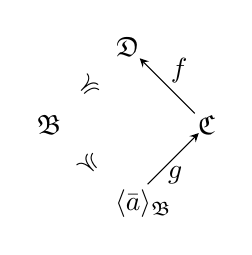
\begin{tikzpicture}
				\draw (0, 1cm) node {$\D$};
				\draw (-1cm, 0) node {$\B$};
				\draw (1cm, 0cm) node {$\C$};
				\draw (0.2cm, -1cm) node {$\langle\bar{a}\rangle_{\B}$};
				
				\path (-1cm, 0) edge [draw=none]
				node [sloped, auto=false,
				allow upside down] {$\preceq$} (0, 1cm);
				
				\draw[-stealth] (0.85cm, 0.15cm) -- (0.15cm, 0.85cm); 
				\draw (0.65cm, 0.7cm) node {$f$};
				
				\path (0, -1cm) edge [draw=none]
				node [sloped, auto=false,
				allow upside down] {$\preceq$} (-1cm, 0);
				
				\draw[-stealth] (0.25cm, -0.75cm) -- (0.9cm, -0.1cm); 
				\draw (0.6, -0.63) node {$g$};
			\end{tikzpicture}
			\label{AmalgamationssatzAbb}
		}
		\hspace{2cm}
		\sidesubfloat[]{
			\begin{tikzpicture}
				\draw (0, 1cm) node {$\D$};
				\draw (-1cm, 0) node {$\B$};
				\draw (1cm, 0cm) node {$\C'$};
				\draw (0cm, -1cm) node {$\A$};
				
				\path (-1cm, 0) edge [draw=none]
				node [sloped, auto=false,
				allow upside down] {$\preceq$} (0, 1cm);
				
				\path (1cm, 0) edge [draw=none]
				node [sloped, auto=false,
				allow upside down] {$\preceq$} (0, 1cm);
				
				\path (0, -1cm) edge [draw=none]
				node [sloped, auto=false,
				allow upside down] {$\preceq$} (-1cm, 0);
				
				\path (0, -1) edge [draw=none]
				node [sloped, auto=false,
				allow upside down] {$\preceq$} (1cm, 0);
			\end{tikzpicture}
			\label{AmalgamationssatzKorollar}
		}
	\caption{Darstellung des Amalgamationssatzes (a) und dessen Folgerung (b)}
\end{figure}

\begin{satz}
	Zu jeder Struktur $\A$ existiert eine elementare Erweiterung $\C$ so, dass Typ $p$ über $A$ in $\C$ realisiert ist.
\end{satz}
\begin{proof}
	Sei $(p_\alpha)_{\alpha<\kappa}$ die Aufzählung aller vollständigen Typen über $A$. Für jedes $\alpha<\kappa$ wählen wir eine elementare Erweiterung $\B_\alpha\succeq\A$ in der $p_\alpha$ realisiert ist.
	Konstruiere eine elementare Kette $(\C_\alpha)_{\alpha<\kappa}$ wie folgt:
	\begin{itemize}
		\item $\C_0\coloneqq\A$.
		\item $\C_\lambda\coloneqq\bigcup_{\alpha<\lambda}C_\alpha$ für Limesordinale $\lambda$.
		\item $\C_{\alpha+1}$ ist eine elementare Erweiterung von $\C_\alpha$ mit der elementaren Einbettung $f:B_\alpha\to\C_{\alpha+1}$ so, dass $f(a)=a$ für $a\in A$.
	\end{itemize}
	Setze $\C\coloneqq\bigcup\limits_{\alpha<\kappa}\C_\alpha(=\C_\kappa)$. $\C$ ist eine elementare Erweiterung aller $C_\alpha$ und damit auch von $\A$ und realisiert jeden Typen über $A$.
\end{proof}

\begin{satz}
	Seien $\B,\C$ $\tau$-Strukturen und $\bar{a}$ ein Tupel aus $B$. Zusätzlich sei $f:\langle\bar{a}\rangle_\B\to\C$ so, dass $\C\models\varphi(f\bar{a})\Rightarrow\B\models\varphi(\bar{a})$ für $\Sigma_1$-Formeln $\varphi(\bar{x})$ gilt. Dann existiert eine elementare Erweiterung $\D\succeq\B$ und eine Einbettung $g:\C\to\D$ mit $gf\bar{a}=\bar{a}$.
\end{satz}
\begin{proof}
	Es lässt sich feststellen, dass $f$ eine Einbettung sein muss. Da $\C\models fa\neq a'\Rightarrow \B\models a\neq a'$ gilt, muss $f$ injektiv sein und betrachtet man $\C\models\neg Rf\bar{x}\Rightarrow\B\models\neg R\bar{a}$ lässt sich feststellen, dass $f$ eine Einbettung ist.
	
	Man nehme nun eine zu $\C$ isomorphe Struktur $\C'$ so, dass $f=\text{id}_{\langle\bar{a}\rangle_\B}$ und $B\cap C'=\langle\bar{a}\rangle_\B$ ist. Sei $T=Th(\B_B)\cup D(\C')$. Zur Erinnerung: $D(C')$ ist das atomare Diagramm von $C'$, also die Menge aller atomaren und negiert-atomaren Formeln, die in $C'$ erfüllt sind. 
	Um zu zeigen, dass $T$ erfüllbar ist, soll wieder der Kompaktheitssatz verwendet werden. 
	Sei $T_0\subseteq T$ also endlich und $\varphi(\bar{a},\bar{c}')$ die Konjunktion der endlich vielen atomaren bzw. negiert-atomaren Formeln aus $T_0\cap D(\C')$ mit $c'\subseteq C'\setminus A$.
	
	Wenn $T_0$ unerfüllbar wäre, dann würde $Th(\B_B)\models\neg\varphi(\bar{a},\bar{c}')$ gelten. Also $Th(\B_B\models\forall\bar{y}\neg\varphi(\bar{a},\bar{y})$. Daraus folgt $\B,\bar{a}\models\neg\exists\bar{y}\varphi(\bar{a},\bar{y})$ und mit der von $f$ geforderten Eigenschaft $\C',\bar{a}\models\neg\exists\bar{y}\varphi(\bar{a},\bar{y})$. Dies ist aber ein Widerspruch zu $\varphi(\bar{a},\bar{c})\in D(\C')$.
	
	Der Rest des Beweises verläuft völlig analog zum Beweis des Amalgamationssatzes.
 \end{proof}
 
 Aus diesem Satz lässt sich folgern, dass für zwei $\tau$-Strukturen $\B$ und $\C$, welche die Eigenschaft erfüllen, dass für beliebige $\Sigma_1$-Sätze $\varphi$ gilt $\C\models\varphi\Rightarrow\B\models\varphi$, sich $\C$ in eine elementare Erweiterung von $\B$ einbetten lässt.

\begin{definition}
	Für $\Phi$ sei $\Phi_\forall\coloneqq\{\varphi\in\Pi_1 : \Phi\models\varphi\}$ und $\Phi_\exists\coloneqq\{\varphi\in\Sigma_1 : \Phi\models\varphi\}$.
\end{definition}

\begin{satz}
	Sei $T\subseteq FO(\tau)$ eine Theorie. Dann gilt $\A\models T_\forall$ gdw. eine Erweiterung $\B\supseteq\A$ existiert, mit $\B\models T$.
	\label{ErweiterungErülltTheorie}
\end{satz}
\begin{proof}
	$\Leftarrow$: $\B\supseteq\A$ mit $\B\models T$ impliziert $\B\models T_\forall$ und da $\Pi_1$-Formeln unter Substrukturen sind und $\B\supseteq\A$, folgt $\A\models T_\forall$.
	
	$\Rightarrow$: Es gelte $\A\models T_\forall$. Behauptung: es gibt ein Modell $\C$ von $Th(\A)_\exists\cup T$. Wenn nicht, dann gibt es eine endliche Teilmenge $\{\varphi_0,\dots,\varphi_{n-1}\}\subseteq Th(\A)_\exists$, welche zusammen mit $T$ unerfüllbar sind. D.h. $T\models \neg\varphi_0\land\dots\land\varphi_{n-1}\eqqcolon\psi\in\Pi_1$. Da also $\psi\in T_\forall$ folgt $\A\models\psi$. Dies steht aber im Widerspruch zu $\A\models\{\varphi_0,\dots,\varphi_{n-1}\}$. Es existiert also solch ein Modell $\C$.
	
	Für jeden $\Sigma_1$-Satz $\varphi$ gilt: $\A\models\varphi\Rightarrow\C\models\varphi$. Also kann man $\A$ eine elementare Erweiterung von $\C$ einbetten. Es gibt also eine Einbettung $f$ so, dass $f(\A)\subseteq\D$ und $\D\succeq\C$ gilt. Es gilt $D\models T$. Also existiert ein $\B\supseteq\A$ mit $\B\models T$.
\end{proof}

\begin{satz}[\L o\'{s}-Tarski]
	Sei $T\subseteq FO(\tau)$ eine Theorie und $\Phi\subseteq FO(\tau)$ eine Satzmenge.
	Dann sind äquivalent:
	\begin{enumerate}
		\item Wenn $\A,\B\models T,\A\subseteq\B$ und $\B\models\Phi$, dann auch $\A\models\Phi$ ($\Phi$ bleibt $\mod T$ unter Substrukturen erhalten).
		\item Es gibt eine Satzmenge $\Psi\subseteq\Pi_1$, die nur aus $\Pi_1$-Sätzen besteht so, dass für jedes Modell von $T$ gilt: $\A\models\Phi\Leftrightarrow\A\models\Psi$ (Auf Modellen von $T$ ist $\Phi$ äquivalent zu einer Menge von universellen Sätzen).
	\end{enumerate}
\end{satz}
\begin{proof}
	\textit{2. $\Rightarrow$ 1.}: Diese Richtung lässt sich leicht mithilfe von Lemma \ref{Pi1UnterSubstruk} einsehen.
	
	\textit{1. $\Rightarrow$ 2.}: Setze $\Psi\coloneqq(T\cup\Phi)_\forall$ und sei $\A\models T$.
	Nun gilt $\A\models\Psi \overset{\text{Satz }\ref{ErweiterungErülltTheorie}}{\Longleftrightarrow}$ es ex. $\B\supseteq\A$ mit $\B\models T\cup \Phi \Rightarrow\A\models\Phi$. Also wenn $\A\models\Phi$ dann auch $\A\models\Psi$.
\end{proof}

Daraus lässt sich die in der Einleitung bereits geschilderte Aussage des Satzes folgern: $\varphi(\bar{x})\in FO(\tau)$ bleibt unter Substrukturen erhalten gdw. $\varphi(\bar)$ äquivalent zu einer Formel $\psi(\bar{x})\in\Pi_1$ ist.
\begin{proof}
	Sei $\bar{c}$ ein Tupel von neuen Konstanten. Betrachte die Theorie $T\coloneqq\{\eta \in FO(\tau\cup\{\bar{c}\}) : \models\eta\}$ aller Tautologien über der Signatur $\tau\cup\{\bar{c}\}$. Wähle $\Phi=\{\varphi(\bar{c})\}$. 
	Aus dem Satz von \L o\'{s}-Tarski folgt, dass $\varphi(\bar{c})$ äquivalent zu einer einer Menge von $\Psi$ von universellen Sätzen ist, also $\Psi\models\varphi(\bar{c})$.
	Nach dem Kompaktheitssatz existiert eine endliche Teilmenge $\Psi_0\subseteq\Psi$ so, dass $\Psi_0\models\varphi(\bar{c})$. Setze $\psi(\bar{c})\coloneqq\bigwedge\Psi_0$. Nun ist $\psi(\bar{c})\equiv\varphi(\bar{c})$, also $\psi(\bar{x})\equiv\varphi(\bar{x})$.
\end{proof}

\begin{definition}[$\kappa$-Saturiertheit]
	Eine Struktur $\A$ ist \textit{$\kappa$-saturiert}, wenn jeder Typ von $\A$ über $B$ mit $\vert B \vert<\kappa$ in $\A$ realisiert ist.
\end{definition}

\begin{satz}
	Jede Struktur $\A$ besitzt eine $\omega$-saturierte elementare Erweiterung $\B\succeq\A$.
\end{satz}
\begin{proof}
	Wir definieren wieder eine Folge $(\B_\alpha)_{\alpha<\omega}$ mit
	\begin{itemize}
		\item $\B_0\coloneqq\A$.
		\item $\B_{\alpha+1}\succeq\B_\alpha$ so, dass in $\B_{\alpha+1}$ jeder Typ von $\B_\alpha$ über eine endlichen Konstantenmenge realisiert ist.
	\end{itemize}
	Nun sei $\B\coloneqq\bigcup_{\alpha<\omega}\B_\alpha$. Weiter sei $p$ ein Typ in $\B$ über einer endlichen Konstantenmenge $C\subseteq B$. Dann ist $C\subseteq B_\alpha$ für ein endliches $\alpha$. Nach Konstruktion ist $p$ dann in $\B_{\alpha+1}$ und damit auch $\B$ realisiert.
\end{proof}

\begin{definition}[Modales Fragment]
	Wir definieren die Abbildung $f:ML\to FO$, welche $ML$-Formeln, in $FO$-Formeln übersetzt. Diese ist induktiv definiert als:
	\begin{itemize}
		\item $f(P_i)\coloneqq P_i x$
		\item $f(\psi_1\circ \psi_2)\coloneqq \psi_1^\ast(x)\circ\psi_2^\ast(x)$ für $\circ\in\{\land,\lor,\rightarrow\}$
		\item $f(\lozenge\psi)\coloneqq\exists y (Exy \land \psi^\ast(y))$
		\item $f(\square\psi) \coloneqq \forall y (Exy\rightarrow \psi^\ast(y))$
	\end{itemize}
	Das \textit{Modale Fragment der Prädikatenlogik} $MF\subseteq FO$ ist definiert als $MF\coloneqq\{\psi^\ast(x) : \exists \psi\in ML (f(\psi)=\psi^\ast(x)) \}$.
\end{definition}

\begin{satz}[van Benthem]
	Es sei $\tau=\{P_i:i\in I\}\cup\{E_a : a\in A\}$, wobei für alle $i\in I$, $P_i$ ein einstelliges und für alle $a\in A$, $E_a$ ein zweistelliges Relationssymbol ist.
	
	Eine Formel $\psi(x)\in FO(\tau)$ ist invariant unter Bisimulation (also wenn $\K\models\psi(v)$ und $\K,v\sim\K',v'$, dann auch $\K'\models\psi(v')$) gdw. $\psi(x)$ äquivalent ist, zu einer Formel $\varphi\in ML$.
\end{satz}
\begin{proof}
	$\Leftarrow$: Diese Richtung wurde bereits in MaLo 1 bewiesen.
	
	$\Rightarrow$: Sei $\psi(x)$ invariant unter Bisimulation und $\Phi\coloneqq\{\varphi(x) \in MF(\tau) : \psi(x)\models\varphi(x)\}$ die Menge der modalen Folgerungen aus $\psi(x)$.
	Wir behaupten nun $\Phi\models \psi(x)$. Sobald wir dies gezeigt haben, folgt der Satz von van Benthem. Denn dann gibt es ein endliches $\Phi_0\subseteq\Phi$ so, dass $\Phi_0\models \psi(x)$. Setzt man dann $\varphi^\ast(x)\coloneqq\bigwedge\Phi_0$ ist $\varphi^\ast$ die Übersetzung einer modalen Formel $\varphi$. $\varphi$ ist äquivalent zu $\psi(x)$.
	\\
	\\
	Sei also $\K_0\models\Phi(v_0)$. Zu zeigen ist, dass $K_0\models\psi(v_0)$. Wir definieren $\Theta\coloneqq\{\psi(x)\}\cup Th_{MF}(\K_0,v_0)$, wobei $Th_{MF}(\K_0,v_0)\coloneqq\{\varphi^\ast(x)\in MF : \K_0\models\varphi^\ast(v_0)\}$ ist.
	
	$\Theta$ ist erfüllbar. Ansonsten existieren $\theta_0(x),\dots,\theta_{n-1}(x)\in Th_{MF}(\K_0,v_0)$ so, dass $\psi(x)\cup\{\theta_0(x),\dots,\theta_{n-1}(x)\}$ unerfüllbar ist. 
	Also ist $\psi(x)\models\neg(\theta_0(x)\land\dots\land\theta_{n-1}(x))$ und damit $\neg(\theta_0(x)\land\dots\land\theta_{n-1}(x))\in\Phi$. Demnach also $\K_0\models\neg(\theta_0(v_0)\land\dots\land\theta_{n-1}(v_0))$. Dies ist aber ein Widerspruch zu $\theta_0(x),\dots,\theta_{n-1}(x)\in Th_Mf(\K_0,v_0)$.
	
	Es gibt also ein Modell $\K_1,v_1$ von $\Theta$.
	Seien $\K_0^+\succeq\K_0,\K_1^+\succeq\K_1$ $\omega$-saturierte Erweiterungen von $\K_0$ bzw. $\K_1$. Weiter ist $Th_{MF}(\K_0^+,v_0)=Th_{MF}(\K_0,v_0)=Th_{MF}(\K_1,v_1)=Th_{MF}(\K_1^+,v_1)$.
	
	Es ist bekannt, dass $\K_0,v_0\sim \K_1,v_1 \Rightarrow \K_0,v_0\equiv_{ML}\K_1,v_1$ gilt. Die Rückrichtung gilt aber nicht im allgemeinen.
	
	\begin{lemma}
		Seien $\K,\K'$ $\omega$-saturiert, mit $\K,v\equiv_{ML}\K',v'$. Dann ist $\K,v\sim\K',v'$.
	\end{lemma}
	\begin{proof}
		Sei $Z=\{(u,u') : \K,u\equiv_{ML} \K',u'\}$. Behauptung: $Z$ ist eine Bisimulation.
		
		Wenn $(u,u')\in Z$, dann ist $\K,u\models P_i\Leftrightarrow \K',u'\models P_i$, für alle $i\in I$.
		
		Hin-Eigenschaft: Sei $(u,w)\in E_a$. Zu zeigen ist, dass es ein $w'$ gibt, mit $(u',w')\in E_a'$ so, dass $(w,w')\in Z$. Wir definieren $p=\{E_a u' x\}\cup Th_{MF}(\K,w)$. $p$ ist ein Typ von $\K'$ über $\{u'\}$. 
		Wenn dies nicht der Fall wäre, dann würde ein endliches $Phi_0\subseteq Th_{ML}(\K,w)$ existieren so, dass $\K'\not\models E_a u' w' \land \bigwedge \Phi_0(w')$ für alle $w'$, bzw. $\K'\models\underbrace{\forall y (E_a u' y \rightarrow \neg \bigwedge\Phi_0(y))}_{\alpha(u')}$. Da wir aber $\K,u\equiv_{ML} \K',u'$ vorausgesetzt haben, folgt $\K\models \alpha(u)$, was aber im Widerspruch steht zu $\K\models E_a u w \land \bigwedge\Phi_0(w)$.
		
		Also ist $p$ realisiert in $\K'$, das heißt, es gibt ein $w'$ mit $\K'\models p(w')$. Also ist $(u',w')\in E_a$ und $\K,w\equiv_{ML} K',w'$. Das heißt $(w,w')\in Z$.
		
		Die Her-Eigenschaft lässt sich völlig analog zeigen.
		
		$Z$ ist also eine Bisimulation. Es folgt $\K,v \sim \K',v'$.
	\end{proof}
	
	Mit diesem Lemma können wir einsehen, dass $\K_0^+,v_0\sim \K_1^+,v_1$.
	Da $\K_1,v_1\preceq \K_1^+,v_1$ und $\K_1\models\psi(v_1)$ folgt $\K_1^+\models\psi(v_1)$. Wegen er Bisimulationsinvarianz von $\psi(x)$ gilt dann auch $\K_0^+\models\psi(v_0)$ und da $\K_0,v_0\preceq\K_0^+,v_0$ folgt $\K_0\models\psi(v_0)$. Dies war zu zeigen.
\end{proof}

Mit diesem Satz lässt sich einsehen, dass die Modallogik $ML$ äquivalent zu dem unter Bisimulation abgeschlossenen Fragment der Prädikatenlogik erster Stufe ist. Im Verlauf des Skriptes wird die weitere Modallogik $L_\eta$ eingeführt werden. 
Nun stellt sich die Frage, ob sich auch für diese eine Logik finden lässt, welches Bisimulationsinvariantes Fragment dieser Modallogik entspricht. 
Mit einem noch komplexeren Beweis als dem Satz von van Benthem lässt sich zeigen, dass genau das für die Monadische Logik zweiter Stufe gilt.

Eine weitere Überlegung die man sich machen kann ist die, ob die beiden diskutierten Erhaltungssätze auch für endliche Strukturen gelten. Es lässt sich zeigen, dass dies für die meisten Sätze nicht gilt. Eine Ausnahme stellt hier der Satz von van Benthem dar. Dieser lässt sich auch für endliche Strukturen benutzen.
Jedoch wird in diesem Fall ein anderer Beweis benötigt, als wir hier verwendet haben. Beispielsweise haben wir mithilfe von $\omega$-saturierten Strukturen argumentiert. Diese sind nach Konstruktion im Allgemeinen nicht endlich
Generell lässt sich auch sagen, dass sehr viel kombinatorischer argumentiert werden muss. Sätze wie den Kompaktsheitssatz kann man beispielsweise nicht anwenden. Über Erhaltungssätze soll nun aber genug gesagt sein.

Weiter soll die infinitäre Logik definiert und die aus MaLo 1 bekannten Ehrenfeucht-Fra\"{i}ss\'{e}-Spiele vollständig hergeleitet werden.




\subsection{Infintäre Logik und Ehrenfeucht-Fra\"{i}ss\'{e}-Spiele}

\begin{definition}
	Sei $\tau$ eine Signatur und $\kappa\in Cn^\infty$. Dann ist die infinitäre Logik $L_{\kappa\omega}[\tau]$ definiert als
	\begin{itemize}
		\item Jede atomare Formel $\varphi\in FO(\tau)$ ist in $L_{\kappa\omega}[\tau]$.
		\item Für $\varphi\in L_{\kappa\omega}[\tau]$ sind $\neg\varphi$, $\exists x \varphi$, $\forall x \varphi\in L_{\kappa\omega}[\tau]$.
		\item $\Phi\subseteq L_{\kappa\omega}[\tau]$ sei eine Formel\textbf{menge} mit $\vert\Phi\vert<\kappa$. Dann sind auch $\bigvee\Phi$ und $\bigwedge \Phi$ Formeln aus $L_{\kappa\omega}[\tau]$.
	\end{itemize}
	Zusammenfassend ist $L_{\infty\omega}[\tau]\coloneqq\bigcup_\kappa L_{\kappa\omega}[\tau]$ definiert.
\end{definition}
Man kann schnell feststellen, dass $L_{\omega\omega}[\tau]=FO(\tau)$ ist.

Um dies besser zu verinnerlichen sollen einige Beispiele erläutert werden:
\begin{itemize}
	\item $\varphi_{fin}\coloneqq\bigvee \{\neg\varphi_{\geq n}: n< \omega\} \in L_{\omega_1\omega}$, mit $\varphi_{\geq n}=\exists x_1\cdots \exists x_n(\bigwedge_{1\leq i < j \leq n}x_i\leq x_j)$. 
	Zuerst soll bemerkt werden, dass in diesem Kontext die Schreibweise $\omega_n$ für $\aleph_n$ verwendet wird. Des weiteren gilt
	$$\mathfrak{A}\models\varphi_{fin} \Leftrightarrow A \text{ endlich}.$$
	
	\item Sei $p$ ein Typ über $B$ mit $\vert B\vert<\kappa$. Dann definieren wir $\varphi(\bar{x})=\bigwedge p$ und es gilt $\A\models \exists \bar{x} \varphi(\bar{x})$, also ist $p$ realisiert in $\A$.
\end{itemize}

\begin{satz}
	Der Kompaktheitssatz gilt nicht für $L_{\kappa\omega}$, wenn $\kappa>\omega$.
\end{satz}
\begin{proof}
	Sei $\varphi_{fin}\in L_{\kappa\omega}$ für $\kappa>\omega$. 
	Dann ist offensichtlich $\Phi=\{\varphi_{fin}\}\cup\{\varphi_{\geq n}:n\in\omega\}$ unerfüllbar, aber jede endliche Teilmenge ist erfüllbar.
\end{proof}

\begin{definition}[Quantorenrang]
	Der aus $FO$ bekannte \textit{Quantorenrang} soll nun auch für die infinitäre Logik $L_{\kappa\omega}$ definiert werden. Für $\psi\in L_{\kappa\omega}$ ist $qr(\psi)\in On$ definiert:
	\begin{itemize}
		\item $\psi$ atomar: $qr(\psi)=0$
		\item $qr(\neg\psi)=qr(\psi)$
		\item $qr(\exists x \psi(x))=qr(\forall x \psi(x))=qr(\psi)+1$
		\item $qr(\bigvee \Phi)=qr(\bigwedge \Phi)\coloneqq \sup\{qr(\varphi):\varphi\in \Phi\}$
	\end{itemize}
\end{definition}

Aich hier sollen wieder Beispiele zum besseren Verständnis angegeben werden:
\begin{itemize}
	\item $qr(\varphi_{fin})=\sup\{qr(\varphi_{\geq n}): n < \omega\}=\omega$.
	\item Sei $\varphi(x)\in L_{\omega_1\omega}(<)$ die Formel, die aussagt, dass $x$ nur endlich viele Vorgänger besitzt. Dann ist $qr(\varphi(x))=\omega$ und $qr(\forall x \varphi(x))=\omega+1$.
\end{itemize}

\begin{definition}[Äquivalenzen]
	Wir schreiben $\A\equiv_\alpha\B$, wenn für alle $\varphi\in L_{\infty\omega}$ mit $qr(\varphi)\leq \alpha$ gilt: $\A\models\varphi \Leftrightarrow \B\models\varphi$.
	
	Analog sei $\A\equiv_\infty\B$, wenn für alle $\varphi\in L_{\infty\omega}$ gilt $\A\models\varphi \Leftrightarrow \B\models\varphi$.
\end{definition}

\begin{definition}[Lokaler Isomorphismus]
	Ein \textit{lokaler Isomorphismus} von $\A$ nach $\B$, für relationale Strukturen $\A$ und $\B$ ist eine Abbildung 
	$p$ mit $Def(p)\subseteq A,Bild(p)\subseteq B$ so, dass $p=\emptyset$ oder
	$p:\A\vert_{Def(p)}\xrightarrow{\sim}\B\vert_{Bild(p)}$. 
	$p$ wird dann auch partieller Isomorphismus genannt.
	
	$Loc(\A,\B)$ beschreibt die Menge aller lokalen Isomorphismen von $\A$ nach $\B$.
\end{definition}

Um lokale Isomorphismen zu notieren werden zwei Notationen verwendet. Seien $\bar{a}=(a_1,a_2,\dots,a_n)$ und $\bar{b}=(b_1,b_2,\dots,b_n)$ so, dass $a_i\in A,b_i\in B$ für $1\leq i \leq n$.
Dann sind $p:\bar{a}\mapsto\bar{b}$ und $p=\{(a_1,b_1),(a_2,b_2),\dots,(a_n,b_n)\}$ zwei Notationen für den Isomorphismus $p$.


\subsubsection*{Spiele}

Nun wollen wir Ehrenfeucht-Fra\"{i}ss\'{e}-Spiele für infinitäre Logiken genauer betrachten.
\begin{definition}[Ehrenfeucht-Fra\"{i}ss\'{e}-Spiele]
	Ein \textit{EF-Spiel} $G_\alpha(\A,\B)$ wird von zwei Spielern gespielt. Dem \textit{Herausforderer (I)} und der \textit{Duplikatorin (II)}. 
	
	Eine \textit{Position} ist ein Tupel $(\beta,\A,\bar{a},\B,\bar{b})$, mit $\beta\leq \alpha$, $\bar{a}\subseteq A$, $\bar{b}\subseteq B$ und $\vert\bar{a}\vert = \vert\bar{b}\vert$.
	Die Startposition ist das Tupel $(\alpha, \A,\langle\rangle,\B,\langle,\rangle)$.
	
	Des weiteren soll nun ein \textit{Zug} von der Position $(\beta,\A,\bar{a},\B,\bar{b})$ aus beschrieben werden: I wählt ein $\gamma < \beta$ und ein $c\in A$ oder $d\in B$. Dann wählt II aus der jeweils anderen Struktur ein $d\in B$ oder $c\in A$. Die neue Position ist dann $(\gamma,\A,\bar{a}c,\B,\bar{b}d)$.
	
	Wird eine Position $(\beta,\A,\bar{a},\B,\bar{b})$ erreicht so, dass $\bar{a}\mapsto\bar{b}\notin Loc(\A,\B)$, dann hat I gewonnen, andernfalls endet das Spiel in einer Position $(0,\A,\bar{a},\B,\bar{b})$ mit $\bar{a}\mapsto\bar{b}\in Loc(\A,\B)$. Dann hat II gewonnen.
\end{definition}

Zur Vereinfachung sagen wir \glqq I/II gewinnt $G_\alpha(\A,\B)$\grqq{} für \glqq I/II hat eine Gewinnstrategie für $G_\alpha(\A,\B)$\grqq{}.

\begin{definition}
	Zusätzlich zu dem Spiel $G_\alpha(\A,\B)$ gibt es das Spiel $G_\infty(\A,\B)$. 
	Dieses verhält sich genauso wie das erstere, bloß wird die erste Komponente der Position weggelassen so, dass Partien unendlich lange dauern können.
	Unendliche Partien sind von II gewonnen.
\end{definition}

\begin{definition}[Hin- und Her-Eigenschaft]
	Sei $I\subseteq Loc(\A,\B)$ und $p\in Loc(\A,\B)$. Dann sagen wir $p$ hat die \textit{Hin- und Her- Eigenschaft (HHE)} bzgl. $I$, wenn gilt:
	\begin{itemize}
		\item Hin: $\forall a\in A \exists b\in B p\cup\{(a,b)\}\in I$
		\item Her: $\forall b\in B\exists a\in A p\cup\{(a,b)\}\in I$
	\end{itemize}
\end{definition}
\begin{definition}[Hin- und Her-System]
	Ein Hin- und Her-System $(I_\alpha(\A,\B))_{\alpha\in On}$ zu $\A$ nach $\B$ besteht aus der Folge von Mengen $I_\alpha(\A,\B)\subseteq Loc(\A,\B)$, welche wie folgt definiert ist:
	\begin{itemize}
		\item $I_0(\A,\B)\coloneqq\{p\in Loc_(\A,\B): p \text{ endlich}\}$
		\item $I_{\alpha+1}\coloneqq\{p\in I_\alpha(\A,\B) : p \text{ hat die HHE bzgl. } I_\alpha(\A,\B)\}$
		\item $I_\delta(\A,\B)\coloneqq \bigcap_{\alpha<\delta}I_\alpha(\A,\B)$ für ein Limesordinal $\delta$.
	\end{itemize}
\end{definition}

Ein HHE-System ist also eine absteigende Kette der Form $I_0(\A,\B)\supseteq I_1(\A,\B) \supseteq \cdots \supseteq I_\alpha(\A,\B) \supseteq I_{\alpha+1}(\A,\B)\supseteq \cdots$.

Auch lässt sich feststellen, dass es ein $\alpha$ gibt so, dass $I_\alpha(\A,\B)=I_{\alpha+1}(\A,\B)$ Wir definieren dann $I_\infty\coloneqq I_\alpha(\A,\B)$.

Weiter gilt für alle $p\in I_\alpha(\A,\B)$ und $q\subseteq p$, dass auch $q\in I_\alpha(\A,\B)$, woraus auch folgt, dass $I_\alpha(\A,\B)\neq\emptyset$ genau dann ist, wenn $\emptyset\in I_\alpha(\A,\B)$.

\begin{definition}
	Um die Notation zu vereinfachen, führen wir folgende Schreibweisen ein:
	\begin{itemize}
		\item $\A\cong_\alpha\B :\Leftrightarrow I_\alpha(\A,\B)\neq\emptyset$
		\item $\A\cong_\infty\B :\Leftrightarrow I_\infty(\A,\B)\neq \emptyset$
	\end{itemize}
\end{definition}

\begin{lemma}
	$\A\cong_\infty\B$ ist genau dann, wenn eine nicht leere Menge $I\subseteq Loc(\A,\B)$ existiert so, dass jedes $p\in I$ die HHE bzgl. $I$ besitzt.
\end{lemma}
\begin{proof}
	$\Rightarrow$: Setze $I=I_\infty(\A,\B)$.
	
	$\Leftarrow$: Sei $J\coloneqq\{p\in I_0(\A,\B) : p\subseteq q \text{ für } q\in I\}$. Dann ist $J\neq\emptyset$ und $J\subseteq I_0(\A,\B)$. Nun hat jedes $p\in J$ die HHE bzgl. $I$ und somit bzgl. jedem $J'\supseteq J$. Daraus folgt direkt $J\subseteq I_\alpha(\A,\B)$ für jedes Ordinal $\alpha$. Also $J\subseteq I_\infty(\A,\B)\neq \emptyset$. Also gilt $\A\cong_\infty\B$.
\end{proof}

Mithilfe von Beispielen sollen HHE-Systeme nun genauer erläutert werden.
\begin{itemize}
	\item[a)] Sei $\A=(\mathbb{Z}, <)$ und $\B=(\mathbb{Q},<)$. Dann ist
	\begin{itemize}
		\item $I_0(\A,\B)=\{\bar{a}\mapsto \bar{b} : \bar{a},\bar{b} \text{endlich}, a_i<a_k \Leftrightarrow b_i<b_k \, \forall i,k\}$
		\item $I_1(\A,\B)=\{\bar{a}\mapsto\bar{b} \in I_0(\A,\B) : \vert a_i-a_k\vert \geq 2 \text{ für } a_i\neq a_k\}$
		\item $I_2(\A,\B)=\{\emptyset\}$
		\item $I_3(\A,\B)=\emptyset$
	\end{itemize}
	
	\item[b)] Sei dagegen nun $\C=(\mathbb{Q},<)$ und $\D=(\R,<)$. Dann ist
	\begin{itemize}
		\item $I_0(\C,\D)=I_0(\A,\B)$
		\item $I_1(\C,\D)=I_0(\C,\D)=I_\infty(\C,\D)$
	\end{itemize}
\end{itemize}

\begin{lemma}
	Seien $\A,\B$ $\tau$-Strukturen, $\bar{a},\bar{b}$ Tupel aus $A$ bzw. $B$ und $\alpha\in On$. Dann gilt:
	
	II gewinnt $G_\alpha(\A,\bar{a},\B,\bar{b})$ gdw. $\bar{a}\mapsto\bar{b}\in I_\alpha(\A,\B)$.
\end{lemma}
\begin{proof}
	Dies soll durch eine Induktion bewiesen werden.
	$\alpha=0$: II gewinnt $G_0(\A,\bar{a},\B,\bar{b}) \Leftrightarrow \bar{a}\mapsto\bar{b}\in Loc(\A,\B) \Leftrightarrow \bar{a}\mapsto\bar{b}\in I_0(\A,\B)$.
	
	$\alpha=\beta+1$:
	\begin{align*}
		&\text{II gewinnt } G_\alpha(\A,\bar{a},\B,\bar{b}) \\
		\Leftrightarrow & (\forall c \in A)(\exists d\in B) \text{II gewinnt } G_\beta(\A,\bar{a}c,\B,\bar{b}d) \land (\forall d \in B)(\exists c\in A) \text{II gewinnt } G_\beta(\A,\bar{a}c,\B,\bar{b}d) \\
		\overset{\text{IV}}{\Leftrightarrow} & (\forall c \in A)(\exists d\in B) \bar{a}c\mapsto\bar{b}d\in I_\beta(\A,\B) \land (\forall d \in B)(\exists c\in A) \bar{a}c\mapsto\bar{b}d\in I_\beta(\A,\B) \\
		\Leftrightarrow& \bar{a}\mapsto\bar{b} \text{ hat HHE bzgl. } I_\beta(\A,\B) \\
		\Leftrightarrow& \bar{a}\mapsto \bar{b}\in I_\alpha(\A,\B).
	\end{align*}
	
	$\alpha$ Limesordinal:
	\begin{align*}
		&\text{II gewinnt } G_\alpha(\A,\B) \\
		\Leftrightarrow & \text{II gewinnt } G_\beta(\A,\B) \forall \beta <\alpha \\
		\overset{\text{IV}}{\Leftrightarrow}& \bar{a}\mapsto\bar{b} \in I_\beta(\A,\B) \forall \beta<\alpha \\
		\Leftrightarrow & \bar{a}\mapsto\bar{b}\in I_\alpha(\A,\B).
	\end{align*}
\end{proof}

Aus diesem Ergebnis lässt sich dann auch leicht folgern, dass $\A\cong_\alpha\B$ genau dann ist, wenn II $G_\alpha(\A,\B)$ gewinnt.

\begin{satz}
	to be continued...
\end{satz}




















\end{document}













